\documentclass{report}

\usepackage{natbib}
\usepackage{mathtools}
\usepackage[a4paper,bindingoffset=0.2in,%
left=1in,right=1in,top=1in,bottom=1in,%
footskip=.5in]{geometry}
\usepackage{listings}
\usepackage{color}
\usepackage{lscape}
\usepackage{hyperref}

\definecolor{darkred}{rgb}{0.26,0.23,0.23}
\definecolor{codegreen}{rgb}{0,0.6,0}
\definecolor{purple}{rgb}{0.65, 0.12, 0.82}

\lstdefinelanguage{JavaScript}{
  keywords={typeof, new, true, false, catch, function, return, null, catch, switch, var, if,  in, while, do, else, case, break},
  keywordstyle=\bfseries,
  ndkeywords={class, export, boolean, throw, implements, import, this},
  ndkeywordstyle=\color{darkgray}\bfseries,
  identifierstyle=\color{black},
  sensitive=false,
  comment=[l]{//},
  morecomment=[s]{/*}{*/},
  commentstyle=\color{purple}\ttfamily,
}

\lstset{ %
  basicstyle=\footnotesize\ttfamily,
  backgroundcolor=\color{white},   % choose the background color; you must add \usepackage{color} or \usepackage{xcolor}; should come as last argument
  breakatwhitespace=false,         % sets if automatic breaks should only happen at whitespace
  breaklines=true,                 % sets automatic line breaking
  captionpos=b,                    % sets the caption-position to bottom
  commentstyle=\color{codegreen},    % comment style
  frame=tb,	                       % adds a frame around the code
  keepspaces=true,                 % keeps spaces in text, useful for keeping indentation of code (possibly needs columns=flexible)
  rulecolor=\color{black},         % if not set, the frame-color may be changed on line-breaks within not-black text (e.g. comments (green here))
  showspaces=false,                % show spaces everywhere adding particular underscores; it overrides 'showstringspaces'
  showstringspaces=false,          % underline spaces within strings only
  showtabs=false,                  % show tabs within strings adding particular underscores
  tabsize=2,	                     % sets default tabsize to 2 spaces
}


%editing
\usepackage{soul}
\usepackage{setspace}

\title{\huge{Emulate \texttt{persp()} plot and \texttt{filled.contour()} plot on \textbf{gridGraphics}}}
\author{\Large{Zhijian Wen} \\ \\ \Large{Supervised by Dr. Paul Murrell}}

\date
{
\vspace{3cm}

\includegraphics[height = 5cm, width = 5cm]{logo.jpg}\\
\vspace{1cm}
% Change to Masters if applicable
Masters of Science\\
Department of Statistics\\
The University of Auckland\\
New Zealand
}



\usepackage{Sweave}
\begin{document}
\setstretch{1.3}
\Sconcordance{concordance:PreReport.tex:PreReport.Rnw:%
1 7 1 1 0 7 1 1 5 10 1 1 6 1 0 4 1 3 0 1 2 10 1 1 2 16 0 1 2 1 4 3 1 1 %
10 2 0 1 2 4 0 1 5 9 1 1 6 1 0 3 1 3 0 1 5 29 1 1 5 1 3 2 0 2 1 5 0 1 1 %
5 0 1 1 5 0 1 1 6 0 1 2 1 4 15 1 1 7 1 0 3 1 1 2 4 0 1 2 10 1 1 2 1 0 1 %
1 1 2 6 0 1 2 6 0 1 2 13 0 1 5 7 1 1 2 1 0 3 1 6 0 1 2 4 1 1 2 1 0 1 1 %
5 0 1 1 6 0 1 2 1 1 1 2 1 0 1 1 1 2 1 0 1 1 6 0 1 2 1 1 1 70 27 1 1 6 1 %
4 3 0 1 1 3 0 1 2 1 4 15 1 11 0 1 10 3 1 11 0 1 10 2 1 24 0 1 23 7 1 1 %
6 1 7 1 4 9 1 1 6 1 9 1 4 13 1 1 7 1 0 1 1 1 7 6 0 1 1 1 2 1 1 5 0 1 1 %
5 0 1 1 5 0 1 1 6 0 1 5 11 1 12 0 1 11 5 1 14 0 1 13 17 1 14 0 1 13 5 1 %
1 6 1 0 5 1 3 0 1 5 8 1 1 2 20 0 1 18 30 1 1 7 2 0 4 1 5 0 1 1 6 0 1 5 %
11 1 1 2 1 0 3 1 1 2 1 0 3 1 4 0 1 3 11 1 1 3 2 0 1 2 1 0 1 3 2 0 1 2 4 %
0 1 2 2 1 1 3 2 0 1 1 1 2 1 0 1 2 1 0 1 1 3 0 1 2 35 1}

\setlength{\parindent}{1pt}
\noindent

\maketitle
\tableofcontents
\listoffigures

\newpage
\section*{Abstract}
The function \texttt{grid.echo()} in the \textbf{gridGraphics} package can be used to converted \textbf{graphics} plot to \textbf{grid} plot. Most of the \textbf{graphics} plot can be convert visually identically. However, there are two kinds of \textbf{graphics}-based plots that \textbf{gridGraphics} cannot replicate: (1) the perspective plot (\texttt{persp()}) for drawing the 3-dimensional surface. (2) The level (contour) plot (\texttt{filled.contour()}) for drawing the filled contour plot. The aim of this paper is to replicate these two kind of plot on \textbf{grid}, then integrate into the \textbf{gridGraphics} package.

\chapter{Introduction}
\section{Background}
The core graphics system in \texttt{R} \citep{R2017} can been divided in to two main packages. The first package is the \textbf{graphics} package. It is older and it provides the original GRZ graphics system from \texttt{S}, sometimes referred to as ''traditional'' graphics. It is relatively fast and many other \texttt{R} packages build on top of it. The newer package is the \textbf{grid} package. It is slower but is has more flexibility and additional features compared to the \textbf{graphics} package. Many other packages are building on top of one of other of these graphics systems. (See Figure \ref{intro}.) \\

\begin{figure}[h]
	\begin{center}
		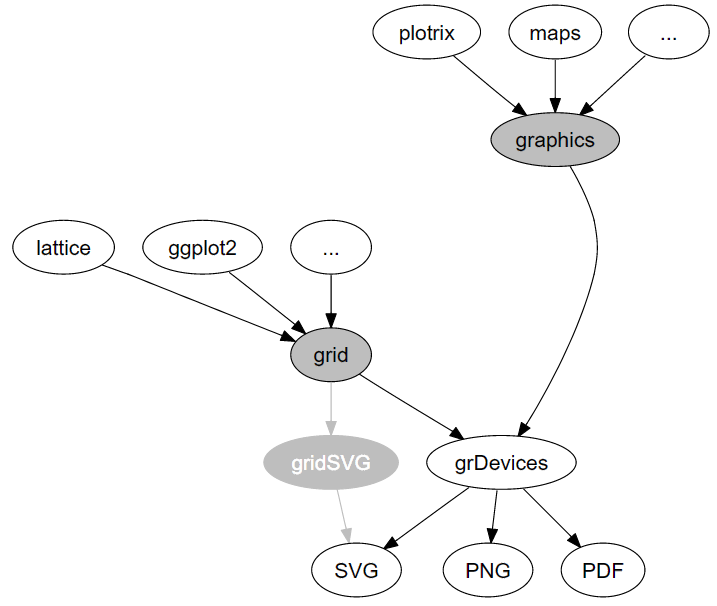
\includegraphics[height = 7.5cm, width = 9.5cm]{figure/intro.png}
		\caption{The structure of the \texttt{R} core graphics system, the \texttt{lattice} \citep{lattice}  and \texttt{ggplot2} \citep{ggplot2} and many others packages are built on top of the \textbf{grid} package. The \texttt{plotrix} \citep{plotrix} and \texttt{maps} \citep{maps} and many others packages are built on top of the \textbf{graphics} package. }
		\label{intro}
	\end{center}
\end{figure}

A graph that is drawn using \textbf{grid} can been edited in many more ways than a graph that has been drawn using the basic \textbf{graphics} package. However, there is a new package, called \textbf{gridGraphics}, which allows us to convert a plot that has been drawn by the \textbf{graphics} package to an equivalent plot drawn by \textbf{grid} graphics. This means that the additional flexibility and features of \textbf{grid} become available for any plot drawn using the \textbf{graphics} package. \\

\section{The \textbf{gridGraphics} package}
The \textbf{gridGraphics} \citep{gGpackage} package acts like a 'translator' that translates a plot that has been drawn using the \textbf{graphics}-based package to a plot that has been drawn using the \textbf{grid} package. \\

The \textbf{gridGraphic} package has a main function called \texttt{grid.echo()}, which takes a recorded plot as an argument (or NULL for the current plot of the current graphics device). The \texttt{grid.echo()} replicates the plot using \textbf{grid} so that the user may edit the plot in more ways than they can with the original plot drawn by basic \texttt{graphic} package.\\

The following code provides a quick example. We generate 25 random numbers for x and y. First, we draw a scatter plot using the function \texttt{plot()} from the basic graphics package, then we redraw it using \texttt{grid.echo()} from the \textbf{gridGraphics} package with \textbf{grid}, See Figure \ref{figure_1.1}
\begin{Schunk}
\begin{Sinput}
> set.seed(110)
> x = runif(25)
> y = runif(25)
> plot(x,y, pch = 16)
> grid.echo()
\end{Sinput}
\end{Schunk}

\begin{figure}[h]
	\begin{center}
		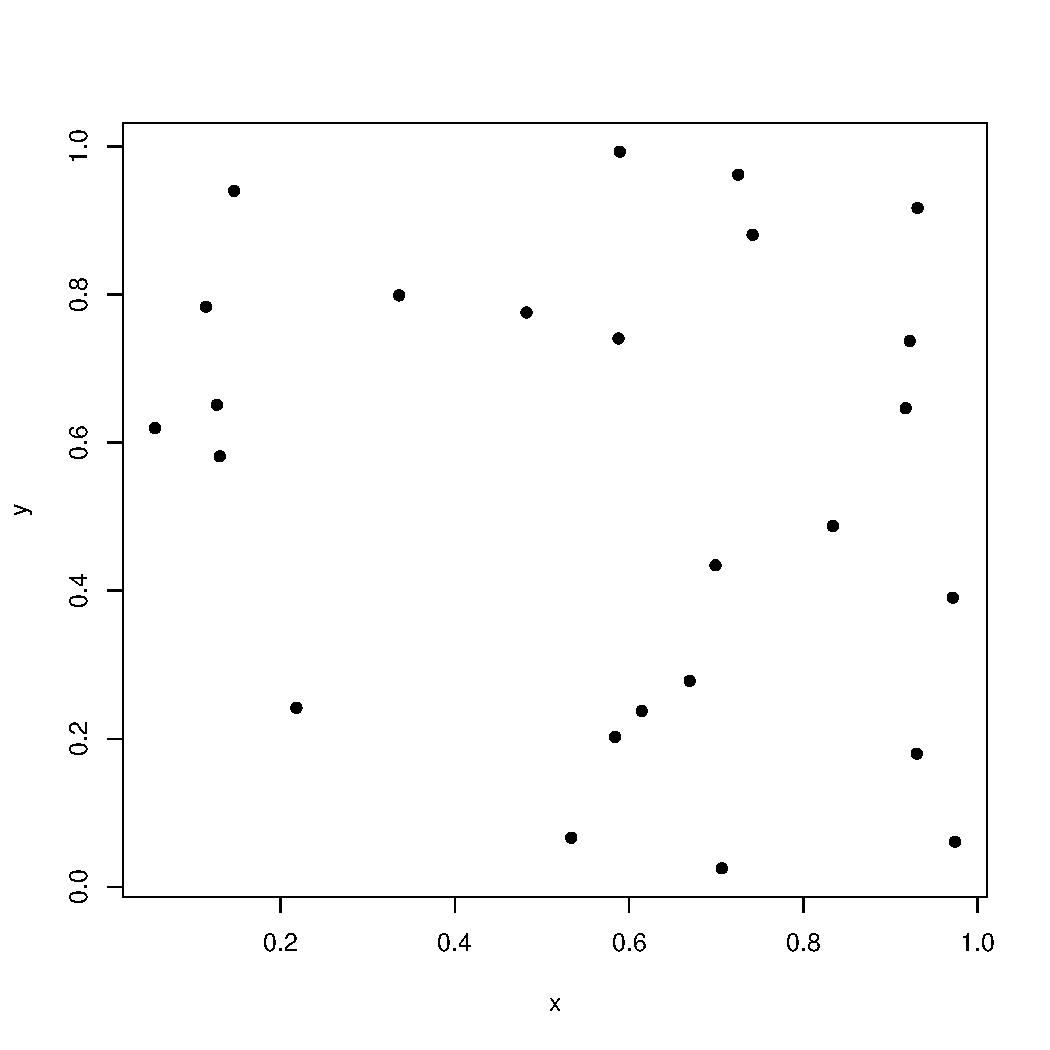
\includegraphics[height = 7.5cm, width = 7.5cm]{figure/report_basic_demo_1.pdf}
		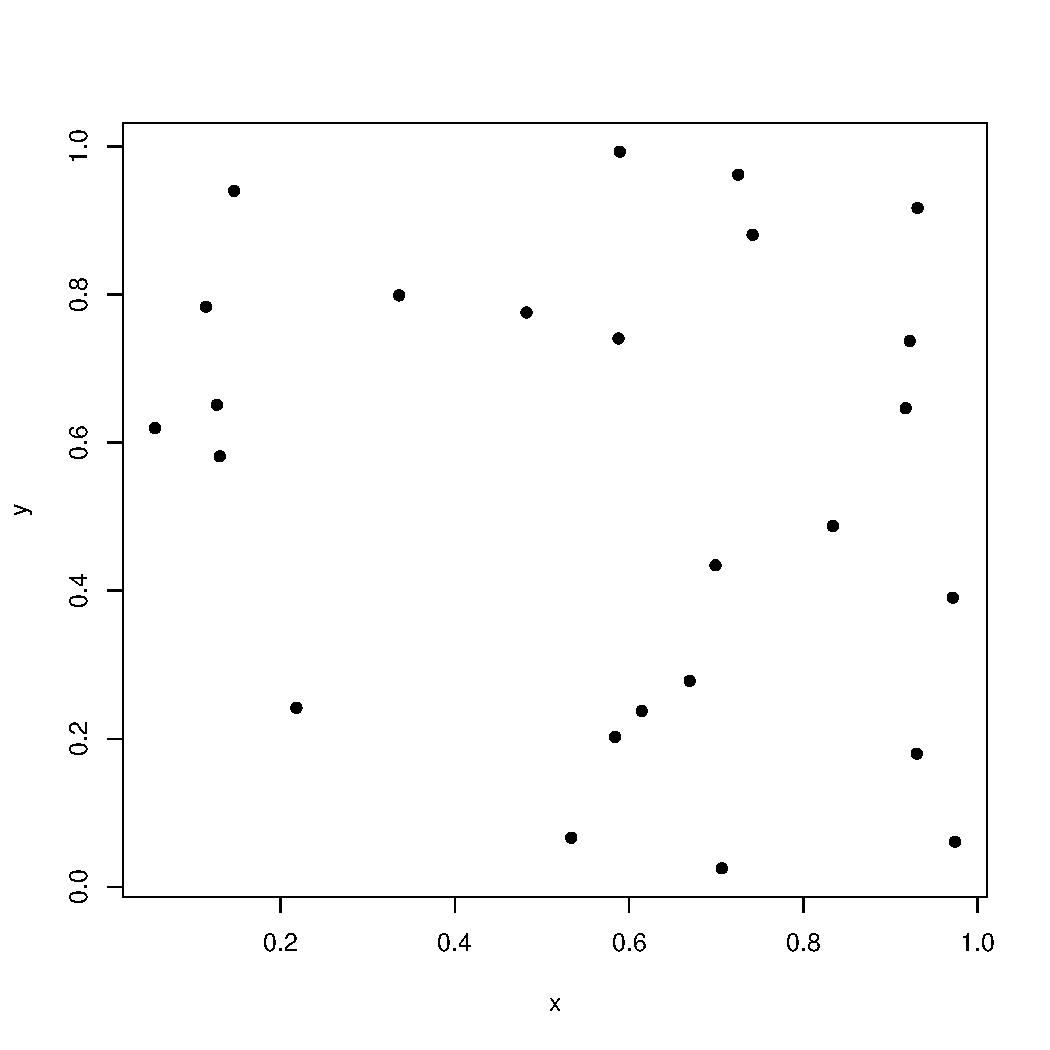
\includegraphics[height = 7.5cm, width = 7.5cm]{figure/report_basic_demo_1.pdf}
		\caption{The left plot is drawn by using \texttt{plot()}; the right plot is redrawn using \texttt{grid.echo()}. Two plots are identical to each other}
		\label{figure_1.1}
	\end{center}
\end{figure}
One example that shows the advantage of drawing the plot using \textbf{grid} rather than basic \textbf{graphics} is that there are objects, called grid grobs, which recorded a list of the details of each components of the plot that has been drawn. The list of grobs can been seen by calling the function \texttt{grid.ls()}. \\
\begin{Schunk}
\begin{Sinput}
> grid.ls()
\end{Sinput}
\begin{Soutput}
graphics-plot-1-points-1
graphics-plot-1-bottom-axis-line-1
graphics-plot-1-bottom-axis-ticks-1
graphics-plot-1-bottom-axis-labels-1
graphics-plot-1-left-axis-line-1
graphics-plot-1-left-axis-ticks-1
graphics-plot-1-left-axis-labels-1
graphics-plot-1-box-1
graphics-plot-1-xlab-1
graphics-plot-1-ylab-1
\end{Soutput}
\end{Schunk}


As we see, the \texttt{grid.ls()} function returns a list of grid grobs for the previous plot that has been redrawn by \textbf{grid}. There is one element called \texttt{graphics-plot-1-bottom-axis-labels-1} which represents the labels of the bottom axis. In \textbf{grid}, there are several functions that can be used to manipulate this grob. See Figure \ref{figure_1.2} \\

For example, if the user wants to rotate the labels of the bottom and left axis by 30 degrees and changes the color from default to orange, then the following code performs these changes.
\begin{Schunk}
\begin{Sinput}
> grid.edit("graphics-plot-1-bottom-axis-labels-1", 
+           rot=30, gp=gpar(col="orange"))
> grid.edit("graphics-plot-1-left-axis-labels-1", 
+           rot=30, gp=gpar(col="orange"))
\end{Sinput}
\end{Schunk}

\begin{figure}[h]
	\begin{center}
		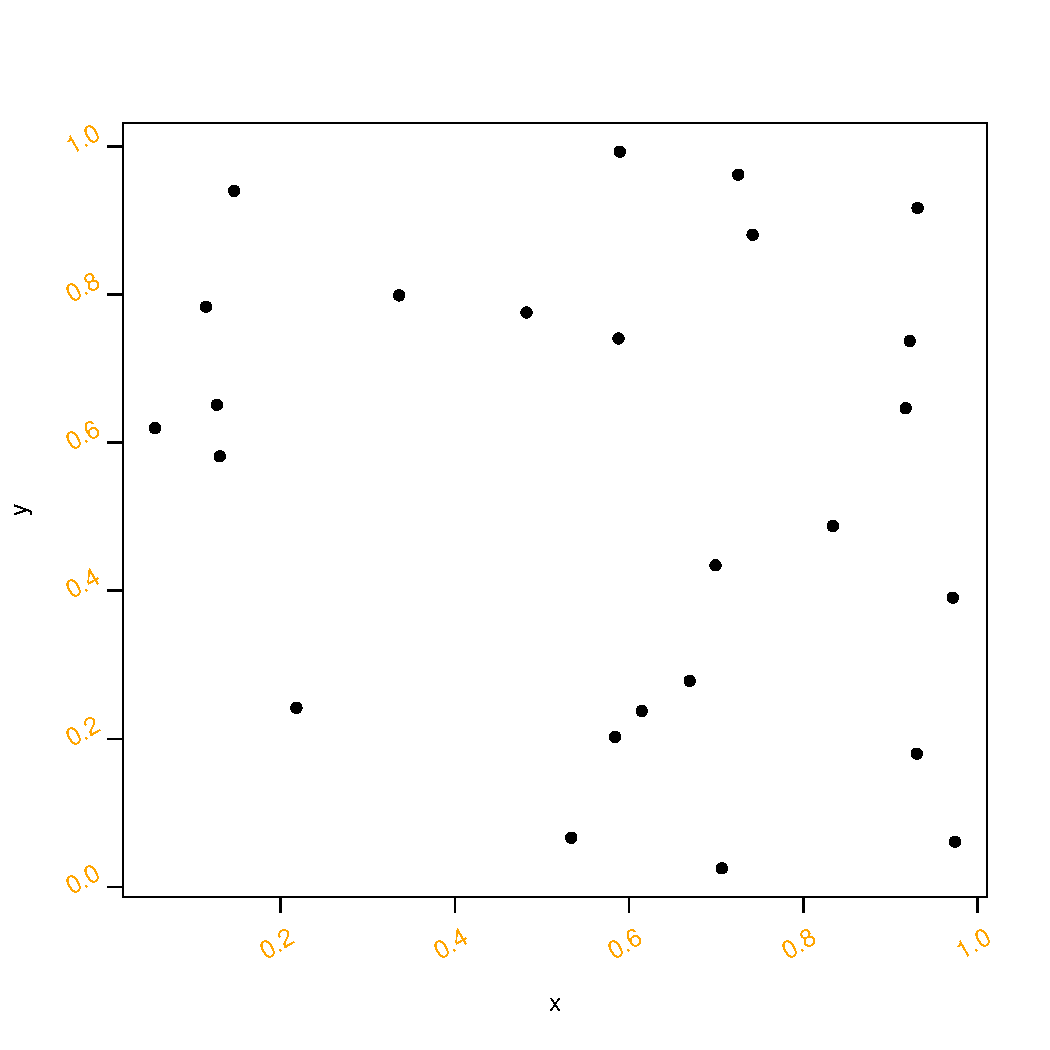
\includegraphics[height = 8cm, width = 8cm]{figure/report_basic_demo_4.pdf}
		\caption{The angle and the color of the bottom and left axis of the previous plot have been changed by 30 degrees and orange}
		\label{figure_1.2}
	\end{center}
\end{figure}
\section{The problem}
The \texttt{grid.echo()} function can replicate most plots that are drawn by the graphics package. However, there are a few functions in the graphics package that \texttt{grid.echo()} cannot replicate. One such function is \texttt{persp()} which draws 3-dimemtional surfaces, the other one is the \texttt{filled.contour()}. If we can draw a plot with \texttt{persp()} or \texttt{filled.countour(),} the result from calling \texttt{grid.echo()} is a (mostly) blank screen. See Figure \ref{figure_1.3}.
\begin{Schunk}
\begin{Sinput}
> x = y = seq(-4*pi, 4*pi, len = 27)
> r = sqrt(outer(x^2, y^2, "+"))
> filled.contour(cos(r^2)*exp(-r/(2*pi)), 
+                frame.plot = FALSE, plot.axes = {})
> grid.echo()
\end{Sinput}
\end{Schunk}
\begin{figure}[h]
	\begin{center}
		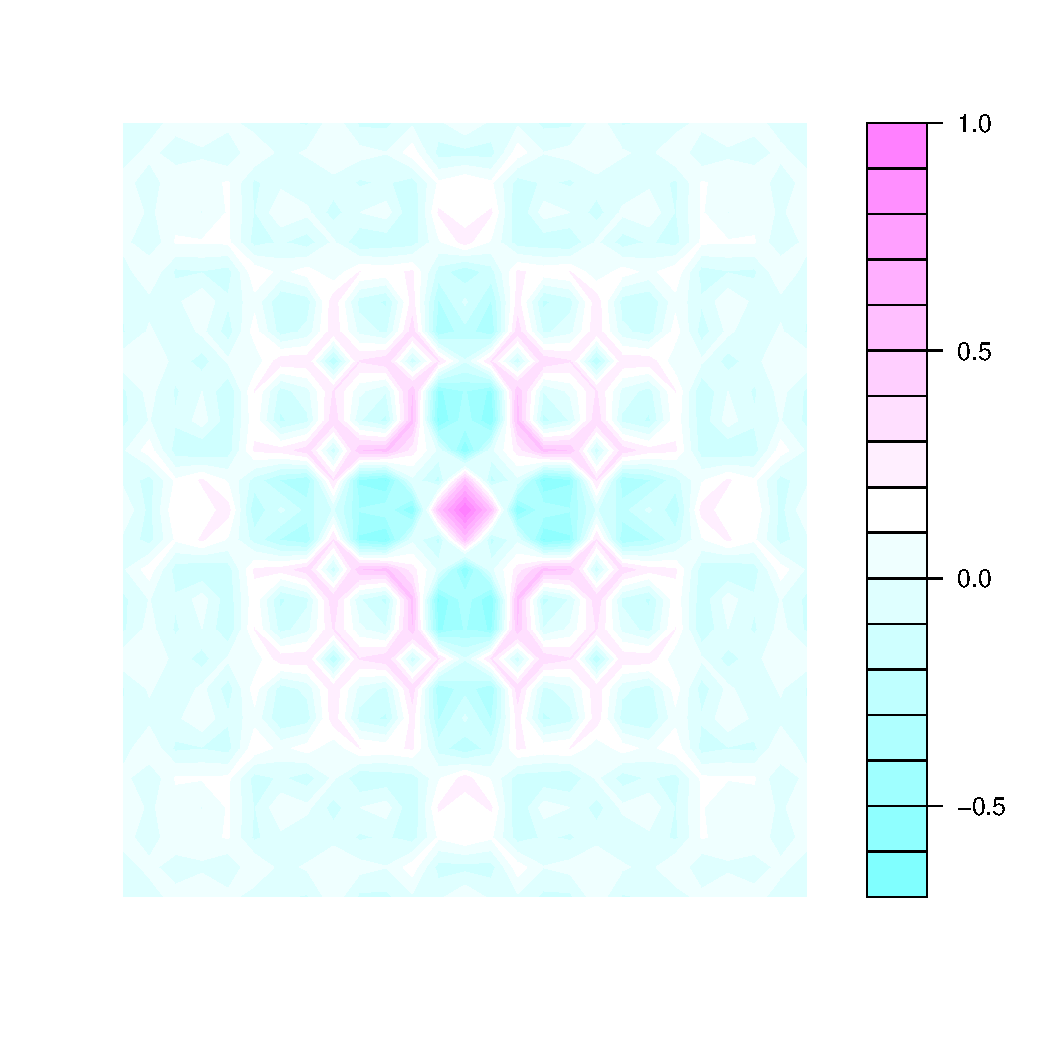
\includegraphics[height = 7.5cm, width = 7.5cm]{figure/report_fill_1}
		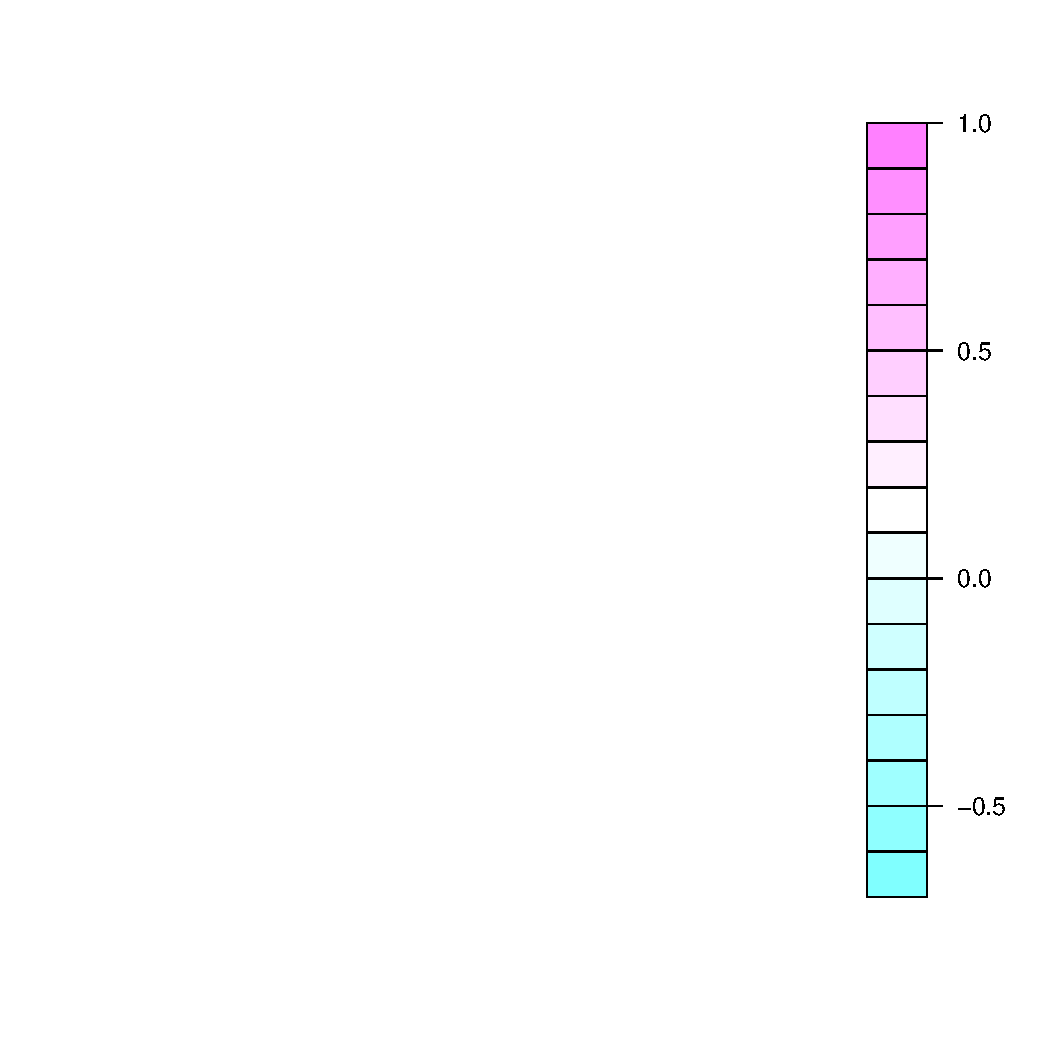
\includegraphics[height = 7.5cm, width = 7.5cm]{figure/report_fill_2}
		\caption{The left plot been drawn by using \texttt{filled.contour()} and the right plot been redrawn by calling \texttt{grid.echo()}. There is a "blank" page on the right plot because the grid.echo cannot emulate \texttt{filled.contour()} in this stage.}
		\label{figure_1.3}
	\end{center}
\end{figure}

\newpage
\section{Aim of this project}
The purpose of this paper is to emulate the Perspective Plots, \texttt{persp()} and Level (Contour) Plots, \texttt{filled.contour()} using the \textbf{grid} package. However, these two functions are written in C, as part of the core \texttt{R} source code. This means that a normal \texttt{R} user or developer cannot modify the code. Also, the \texttt{C} code is structured so that the normal \texttt{R} user or developer cannot separately call the \texttt{C} code. The solution of this paper as follows: 

\begin{enumerate}
	\item Emulate the \texttt{persp()} function on \textbf{grid} separate from the \textbf{gridGraphics} package (standalone):
	\begin{enumerate}
		\item Extract the information from the graphics engine display list.
		\item Understanding and translating the calculation that been done by \texttt{C} code from the \textbf{graphics} package to \texttt{R} code
		\item Draw the Perspective Plot and Filled Contour Plot on \textbf{grid}.
	\end{enumerate}
	\item Integrate the standalone to the \textbf{gridGraphics}
		\begin{enumerate}
			\item Navigating to the correct viewport that has been set up by \textbf{gridGraphics}
			\item Create a new viewport for setting up the correct x-scale and y-scale preparing for drawing, (if necessary) then draw the contents in the correct viewport.
			\item Test the identicality of the plots that been drawn by \textbf{graphics} and \textbf{grid}
		\end{enumerate}
\end{enumerate}



% NOTE to Jason: explain how gridGraphics works first: graphics display list; gridGraphics implements an R version of each low-level C function on the display list (e.g., for C\_plot\_xy there is an R function called C\_plot\_xy in the gridGraphics package). THEN maybe write about 3D to 2D transformations, but only maybe.% 


\chapter{The graphics engine display list}
The information for every plot drawn by R can saved as a \texttt{R} object. For example, In the simple \texttt{plot()} function, it is possible to obtain the parameters for x and y, even the label of the x-axis and y-axis. See Figure \ref{figure_2.1}.\\

This information is called the graphics engine display list. In this paper, we use the graphics engine display list to replicate the \texttt{persp()} plot and \texttt{filled.contour()} plot using grid. The \texttt{recordPlot()} function can be used to access the graphics engine display list and saved as an \texttt{R} object.

\begin{Schunk}
\begin{Sinput}
> plot(cars$speed, cars$dist, col = 'orange', 
+       pch = 16, xlab = 'speed', ylab = 'dist')
> reco = recordPlot()[[1]][[4]][[2]][[2]]
> head(reco[[1]]) #x
\end{Sinput}
\begin{Soutput}
[1] 4 4 7 7 8 9
\end{Soutput}
\begin{Sinput}
> head(reco[[2]]) #y
\end{Sinput}
\begin{Soutput}
[1]  2 10  4 22 16 10
\end{Soutput}
\begin{Sinput}
> reco$xlab
\end{Sinput}
\begin{Soutput}
[1] "cars$speed"
\end{Soutput}
\begin{Sinput}
> reco$ylab
\end{Sinput}
\begin{Soutput}
[1] "cars$dist"
\end{Soutput}
\end{Schunk}


\begin{figure}[h]
	\begin{center}
		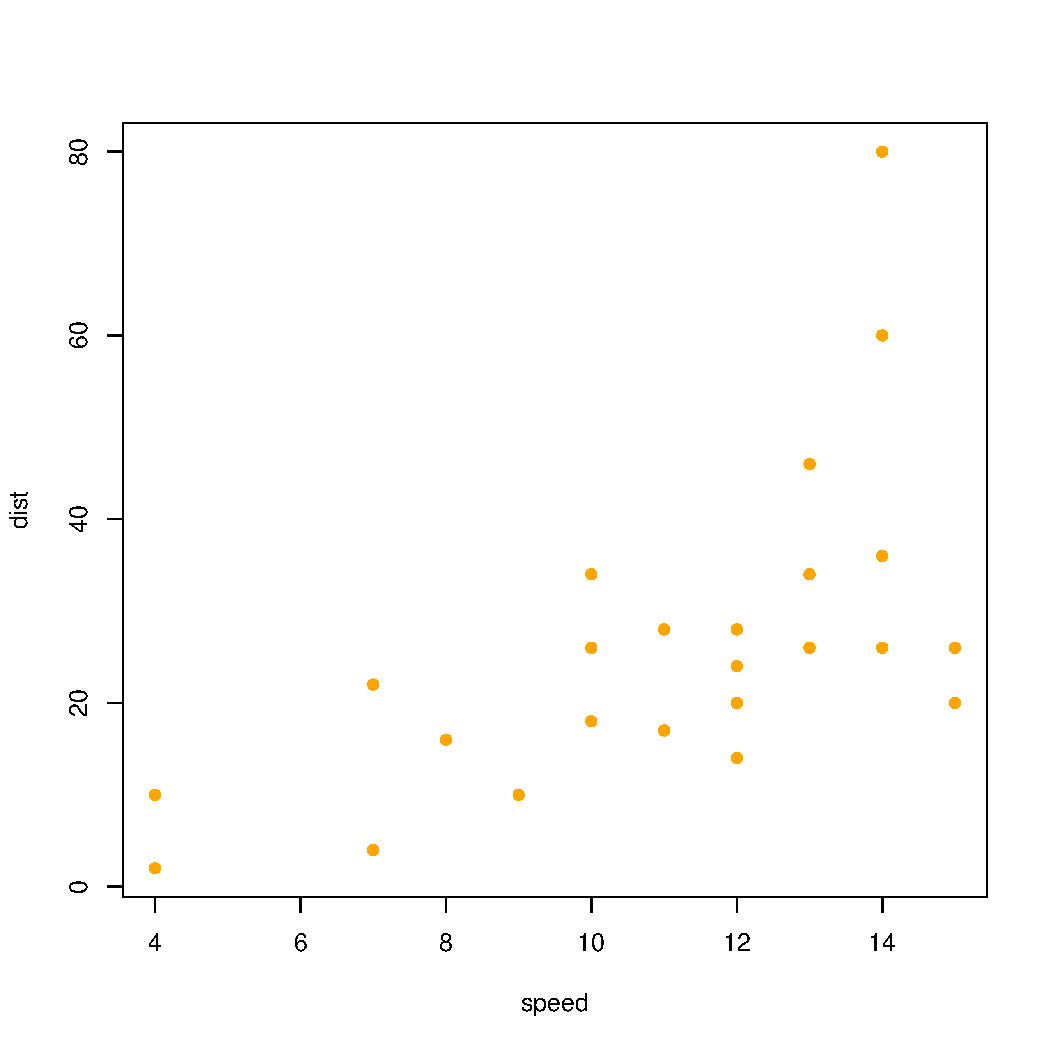
\includegraphics[height = 10cm, width = 10cm]{figure/report_3.pdf}
		\caption{The details of the plot of dist vs speed displayed by the graphics engine display list}
		\label{figure_2.1}
	\end{center}
\end{figure}

The example demonstrates how to access the graphics engine display list of a plot drawn by \texttt{plot}. The values of x and y, the labels of x-axis and y-axis are displayed.



\chapter{Standalone}
\section{The Perspective Plots \texttt{persp()}}
The Perspective Plots \texttt{persp()} is used to draw a surface over the x-y plane.  
It has three main argument, \textbf{x, y, z}. Where \textbf{x} and \textbf{y} are the locations of grid line. The \textbf{z} is a matrix which contains the values that been used to plot, or it is the matrix that been calculated by a specific function, such as 3-D mathematical functions. The example (See Figure \ref{figure_3.1}) shows how to draw an obligatory mathematical surface rotated sinc function on Perspective Plot.
\begin{Schunk}
\begin{Sinput}
> x = y = seq(-10, 10, length= 40)
> f = function(x, y) { r = sqrt(x^2+y^2); 10 * sin(r)/r }
> z = outer(x, y, f)
> z[is.na(z)] = 1
> trans = persp(x, y, z, theta=30, phi = 20, expand = 0.5,
+               col = 'White', border = 'orange')
\end{Sinput}
\end{Schunk}
\begin{figure}[h!]
	\begin{center}
		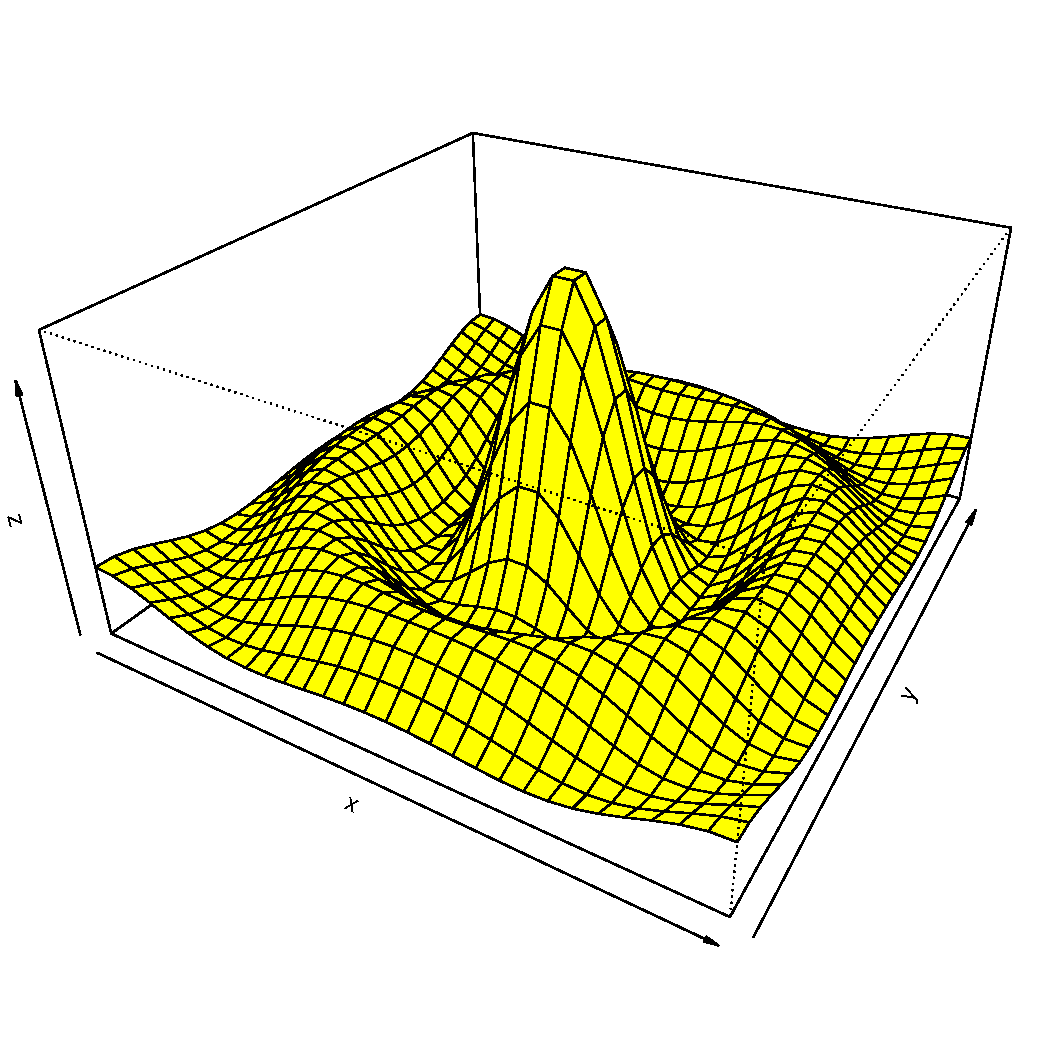
\includegraphics[height = 8cm, width = 8cm]{figure/standalone_1.pdf}
		\caption{A sinc surface drawn by \texttt{persp()}}
		\label{figure_3.1}
	\end{center}
\end{figure}

The sinc surface is built up by finite number of "polygon", each polygon has 4 Vertices.
If we can access the coordinates one polygon, then we can redraw this polygon on \textbf{grid}. If we can access all the coordinates of all polygons, then we can emulate the Perspective Plot on \textbf{grid}. The following codes show that the value of \textbf{x}, \textbf{y} and \textbf{z} which inputted by the user can been " caught " from the display list.
\begin{Schunk}
\begin{Sinput}
> reco = recordPlot()
> info = reco[[1]][[3]][[2]]
> ## print the values of x
> head(info[[2]])
\end{Sinput}
\begin{Soutput}
[1] -10.000000  -9.487179  -8.974359  -8.461538  -7.948718  -7.435897
\end{Soutput}
\begin{Sinput}
> ## print the values of y
> head(info[[3]])
\end{Sinput}
\begin{Soutput}
[1] -10.000000  -9.487179  -8.974359  -8.461538  -7.948718  -7.435897
\end{Soutput}
\begin{Sinput}
> ## print the values of z
> info[[4]][1:6, 1:2]
\end{Sinput}
\begin{Soutput}
            [,1]       [,2]
[1,]  0.70709805  0.6807616
[2,]  0.68076162  0.5602102
[3,]  0.56890062  0.3623630
[4,]  0.38799490  0.1144364
[5,]  0.16158290 -0.1521360
[6,] -0.08388565 -0.4067000
\end{Soutput}
\end{Schunk}
\subsection{Convert the inputs into the coordinates of vertices}
The inputs(\textbf{x}, \textbf{y} and \textbf{z}) are recorded by \texttt{recordPlot}. However, we cannot draw the surface directly by using the inputs, because the inputs are not the vertices coordinates of the surface. Therefore, the first step is to convert these \textbf{x}, \textbf{y} and \textbf{z} inputs into the coordinates of the vertices of every polygon.


As we know, the matrix, \textbf{z} is computed by a specific functions, given two inputs, \textbf{x} and \textbf{y}, or the expression of z can been written as: $z = f(x,y)$, it contains all the values for all combination of \empth{x} and \textbf{y} and the dimension of \textbf{z} is $ \textbf{length(x)} \times \textbf{length(y)}$.\\

One 3-dimenstions points contains a set values of (\textbf{x}, \textbf{y}, \textbf{z}). However, \textbf{z} is $\textbf{length(x)} \times \textbf{length(y)}$ matrix, \textbf{x} is a vector which has length of $\textbf{length(x)}$ and \textbf{y} is a vector which has length of $\textbf{length(y)}$. To produce the points, the coordinates (\textbf{x}, \textbf{y} and \textbf{z}) need to be matched in a right order.\\

First step is the reduce the \textbf{z} matrix into a one dimension vector which has length of $\textbf{length(x)} \times \textbf{length(y)}$. It can be reduced by either along x direction or y direction. In this paper, we reduced along the x direction. The second step is repeat the vector x and y until the same length of \textbf{z}. Since \textbf{z} is reduced along the x direction say $z_p$, we repeat x until the length of y say $x_p$, and we repeat each y by the length of \textbf{x}, say $y_p$. At last, the combination of $x_p$, $y_p$, $z_p$ is the 3-D points which prepare for computing the vertices. \\
\begin{Schunk}
\begin{Sinput}
> xTmp = rep(x, length(y))
> yTmp = rep(y,each = length(x))
> zTmp = as.numeric(z)
> length(xTmp) == length(zTmp) & length(yTmp) == length(zTmp)
\end{Sinput}
\begin{Soutput}
[1] TRUE
\end{Soutput}
\end{Schunk}

Converting points to vertices by repeating the points in a right order. From previous section, we explained that the Perspective Plots is made by finite number of polygons. Each polygon has 4 vertices. The total number of polygons are required to be drawn is depend on the length of input \textbf{x} and the length of input \textbf{y}, that is, total = (length(x) - 1) $\times$ (length(y) - 1). The polygons been drawn by connecting 4 points in a specific order. The order of the drawing as follows: starting from bottom-left, (1) connect bottom-left to bottom-right, (2) connect from bottom-right to top-right, lastly, (3) connect top-right to top-left, (4) connect top-left to bottom-left. Every polygon is being drawn in this order. The surface of Perspective Plots is formed until all the polygons are been drawn. \\

\subsection{The transformation from 3-D vertices into 2-D vertices}
Before drawing the surface, the transformation of 3-D vertices into 2-D vertices is required. This transformation required two main variables, the 3-D vertices and a transformation matrix \textbf{P}. The 3-dimenstion vertices are already computed, \textbf{P} is a 4 by 4 viewing transformation matrix which suitable for projecting 3-dimensions coordinates (x, y, z) into 2-dimensions plane using homogeneous 4-dimension coordinates (x, y, z, t). It can be recorded from the \texttt{persp()} call. This transformation can be done easily on R by using the \texttt{trans3d()} function.

\begin{Schunk}
\begin{Sinput}
> points3d = trans3d(xTmp, yTmp, zTmp, trans)
> head(points3d$x)
\end{Sinput}
\begin{Soutput}
[1] -0.3929051 -0.3827005 -0.3720915 -0.3611435 -0.3499392 -0.3385634
\end{Soutput}
\begin{Sinput}
> head(points3d$y)
\end{Sinput}
\begin{Soutput}
[1] -0.1060481 -0.1099038 -0.1156894 -0.1230654 -0.1315269 -0.1404974
\end{Soutput}
\end{Schunk}

Some polygons that stay 'behind' cannot been seen, it is necessary to draw the polygons in a right order. That is, draw the polygons which located further behind first then draw the polygons which located font, from user's view. The order defined by using the \textbf{x} and \textbf{y} coordinate of the 3-D vertices (but ignore the \textbf{z} coordinate) combining another column \textbf{1}, then do the matrix multiplication with the viewing transformation \textbf{P}. The fourth column from this multiplication is the order of the polygons. The following codes calculated the order of every polygons where \texttt{a} indicates the orders.
\begin{Schunk}
\begin{Sinput}
> orderTemp = cbind(xTmp, yTmp, 0, 1) %*% trans 
> zdepth = orderTemp[, 4]
> ## the zdepth of a set of 4 points of each polygon
> a = order(zdepth, decreasing = TRUE)
> head(a)
\end{Sinput}
\begin{Soutput}
[1] 1561 1562 1521 1563 1522 1564
\end{Soutput}
\end{Schunk}

Figure \ref{figure_3.2} shows how does this paper approximate to the solution. The top-left figure is drawn by plotting the transformed 2-dimenstion points, the shape of the Perspective Plots been presented. The top-right figure is drawn by connecting the points line-by-line, the shape become more obvious. The bottom-left figure is drawn by using the \texttt{grid.polygon()}. By default, the origin order of the polygons is drawn along x-axis, then along y-axis. Clearly this is not the correct order. Finally, the bottom-right figure shows the true Perspective Plots by fixing the order. 
\begin{figure}[h]
	\begin{center}
		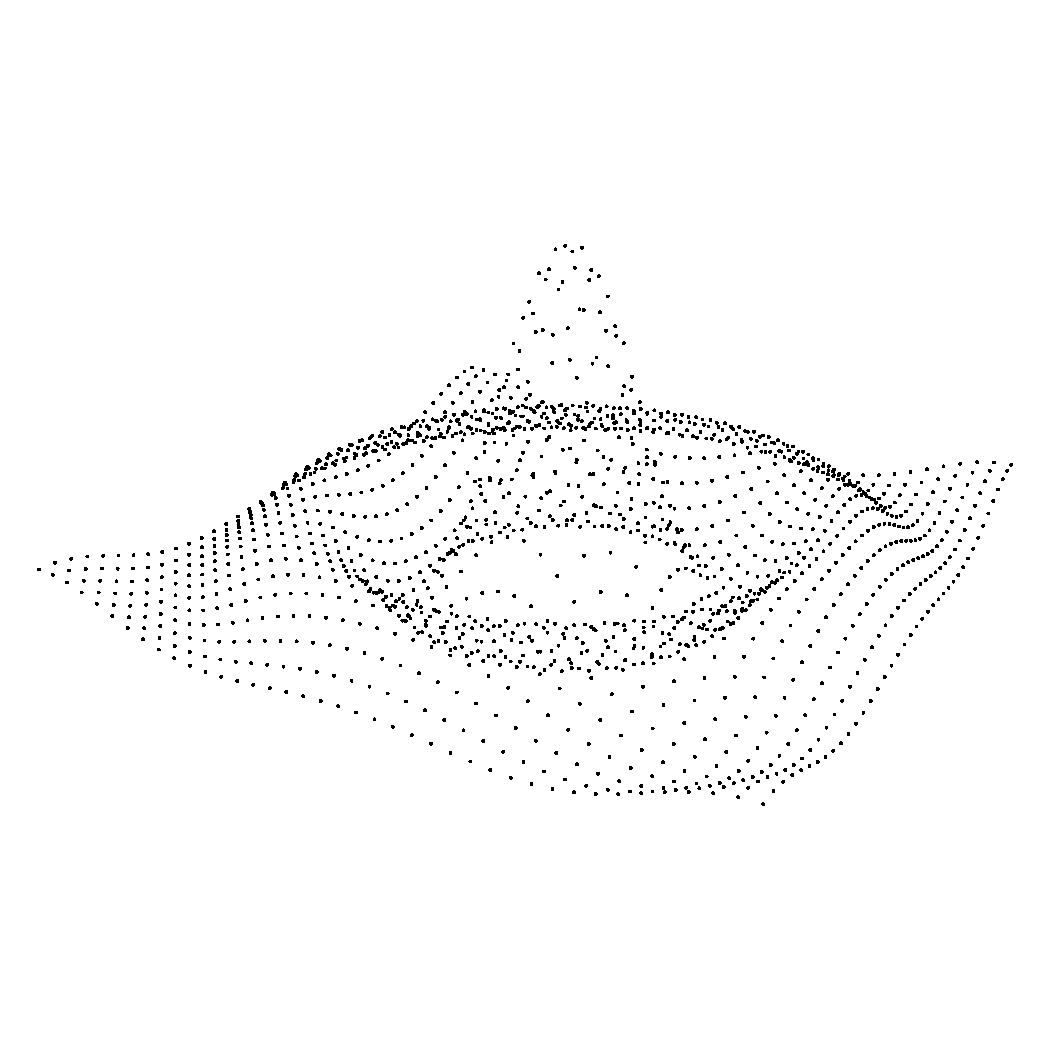
\includegraphics[height = 7.5cm, width = 7.5cm]{figure/standalone_p_1.pdf}
		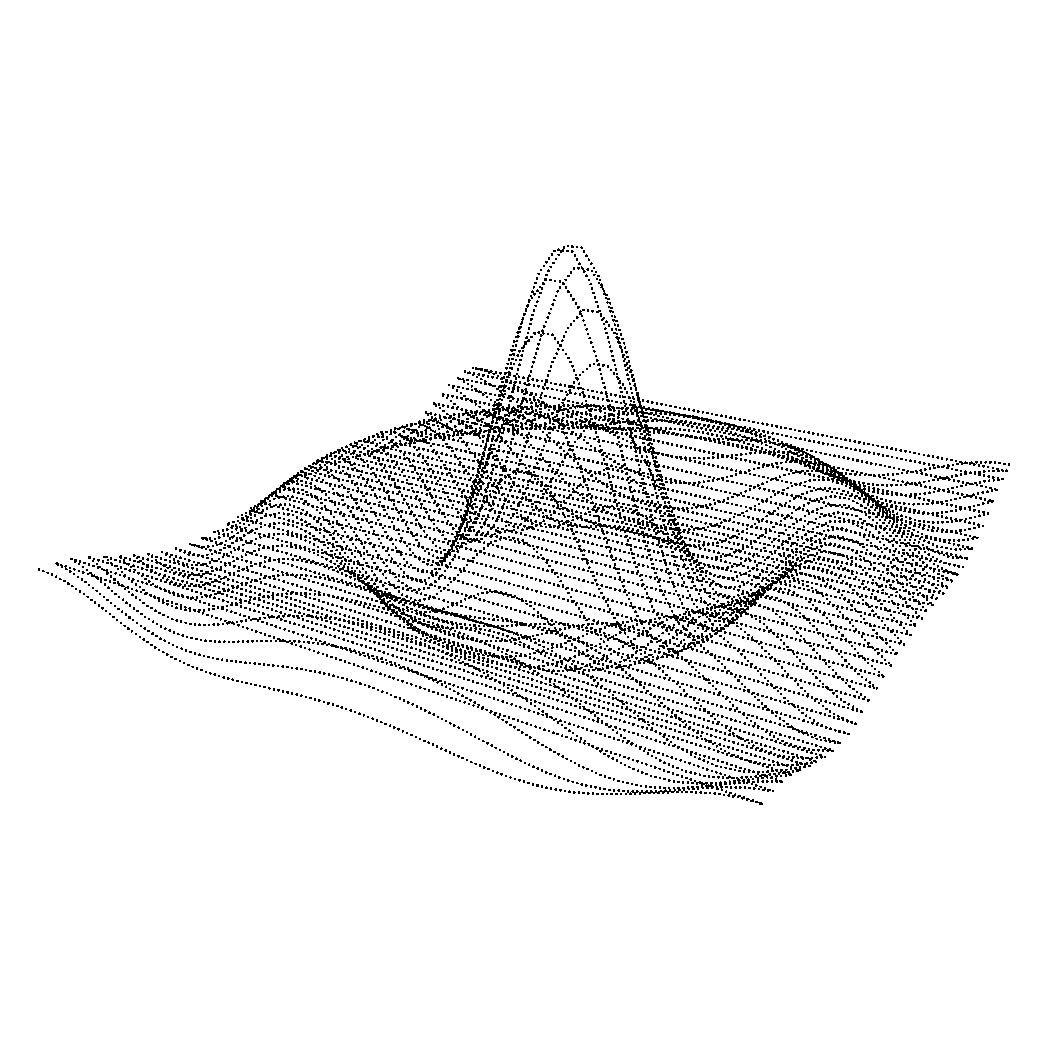
\includegraphics[height = 7.5cm, width = 7.5cm]{figure/standalone_p_2.pdf}
		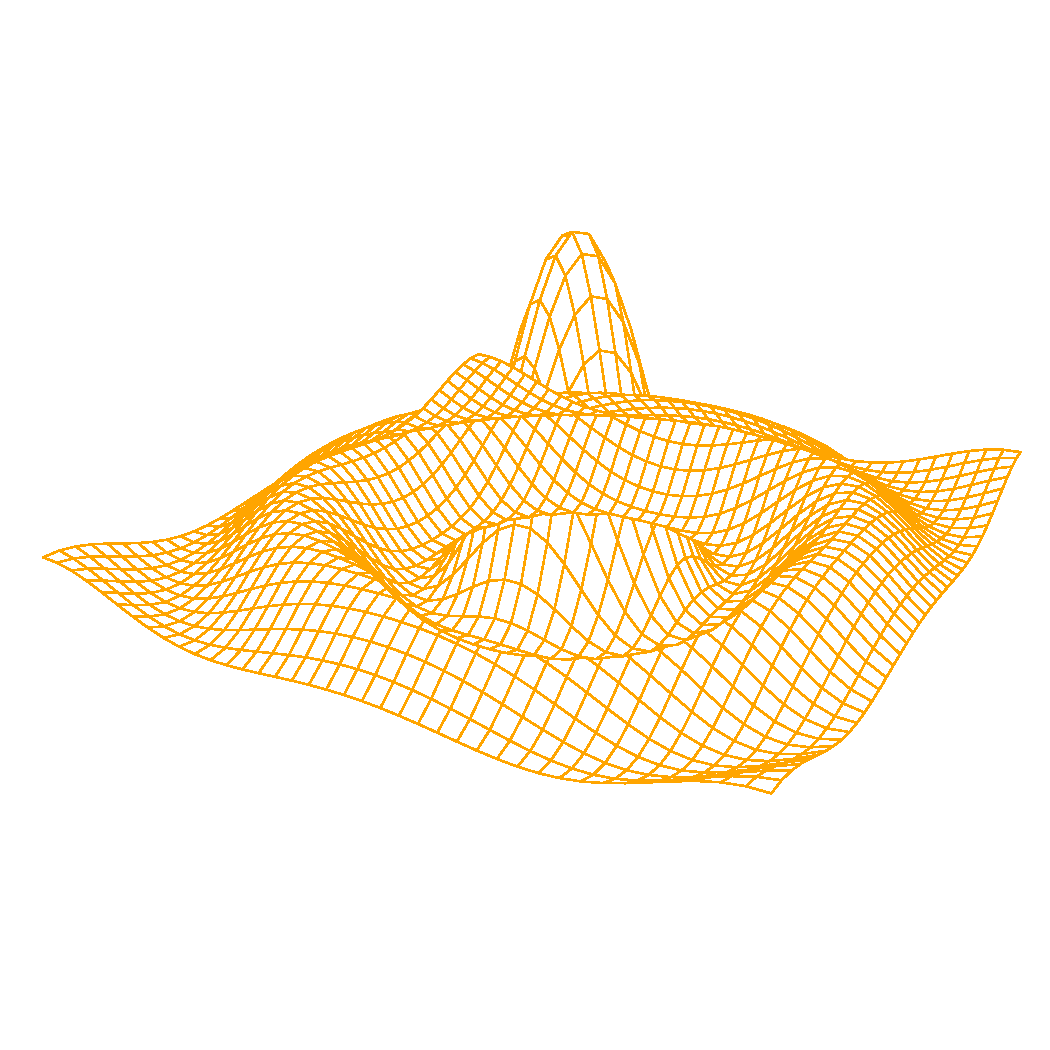
\includegraphics[height = 7.5cm, width = 7.5cm]{figure/standalone_p_3.pdf}
		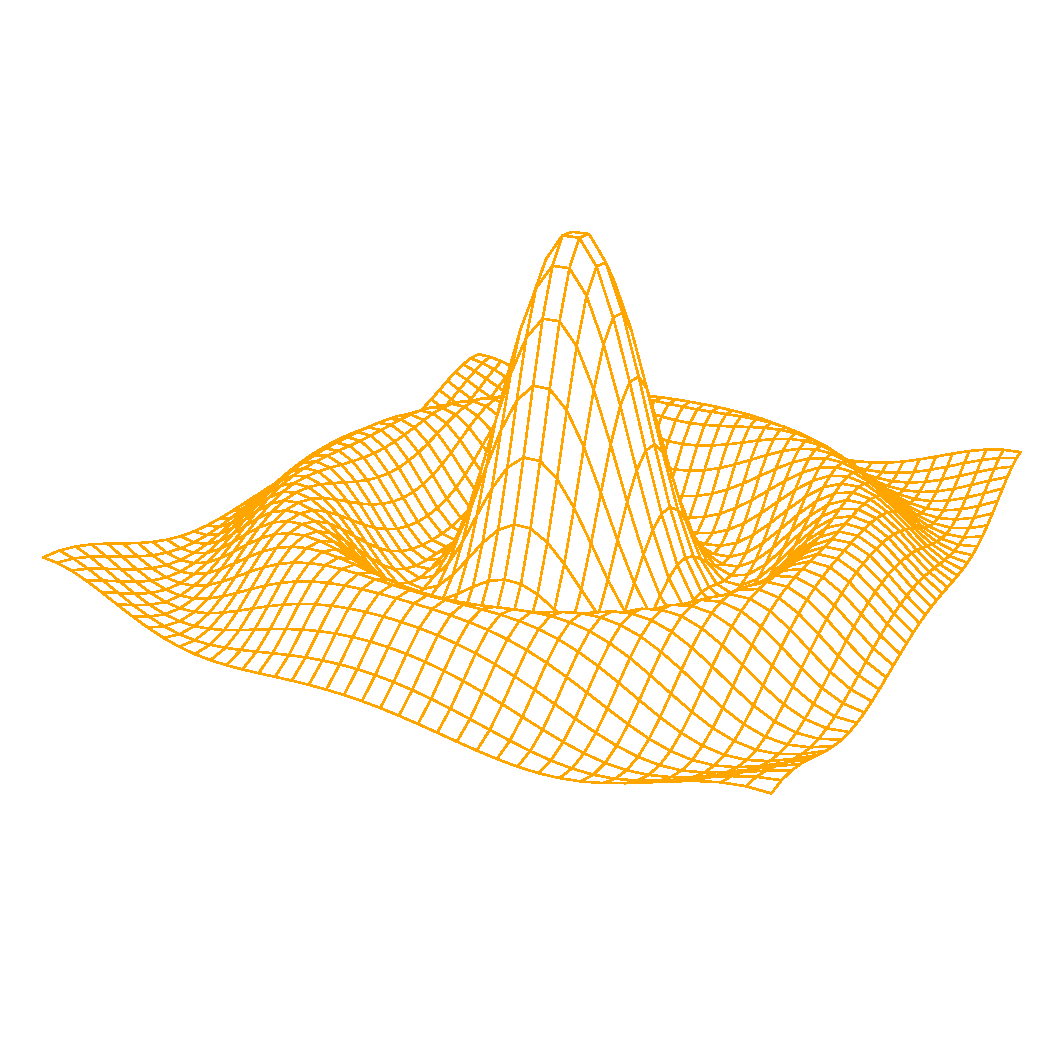
\includegraphics[height = 7.5cm, width = 7.5cm]{figure/standalone_p_4.pdf}
		\caption{The top-left figure is only plotting the transformed 2-dimenstion points. The top-right figure is being drawn by connecting the points line-by-line. The top-right figure is drawn unorderly by using the \testtt{grid.polygon}. Finally, the bottom-left figure is drawn in a correct order.}
		\label{figure_3.2}
	\end{center}
\end{figure}

\subsection{Lighting}
The other main benefit supported by \texttt{persp()} is the shading. It shades the surface by assuming the surface is being illuminated from a given direction. (light source). In \texttt{persp()}, the main parameters that the user needs to specify for producing a shaded perspective plot is: \textbf{ltheta}, \textbf{lphi} and \textbf{shade}. The \textbf{ltheta} and \textbf{lphi} are used for setting up the direction of the light source. In particular, \textbf{ltheta} specifies the angle in the z direction, \textbf{lphi} specifies the angle in the x direction. \textbf{s} is the parameter that specifies the shade at each facets of the surface, and the shades will be computed as follows:
\begin{equation}
Shade = \big(\frac{1 + d}{2}\big)^{s}
\end{equation}
Where \textbf{d} is the dot product of the unit vector normal to each facet(\textbf{u}) and the unit vector of the direction of the light(\textbf{v}). \\

The color of each facet will be calculated by the color that is recorded from the graphics engine display list multiplied by the \textbf{shade}. Finally, the surface is drawn by filling the colors for every facet.\\

If the normal vector is perpendicular to the direction of the light source, then $d = 0$ and the \textbf{shade} will be close to 0, therefore the corresponding facets will become darker. The brightness and darkness will depend on the value of the \textbf{s}. If \textbf{s} close to 0, the \textbf{Shade} will be close to 1. Therefore, it will look like non-shading plot. Similarly, if the \textbf{s} gets larger, the \textbf{Shade} close to 0 and the plot will look darker.

\begin{Schunk}
\begin{Sinput}
> trans = persp(x, y, z, theta=30, phi = 20, expand = 0.5,
+               col = 'white', border = 'orange')
> trans = persp(x, y, z, theta=30, phi = 20, expand = 0.5,
+               col = 'white', border = 'orange', 
+               shade = 0.8, ltheta = 30, lphi = 20)
\end{Sinput}
\end{Schunk}


\begin{figure}[h]
	\begin{center}
		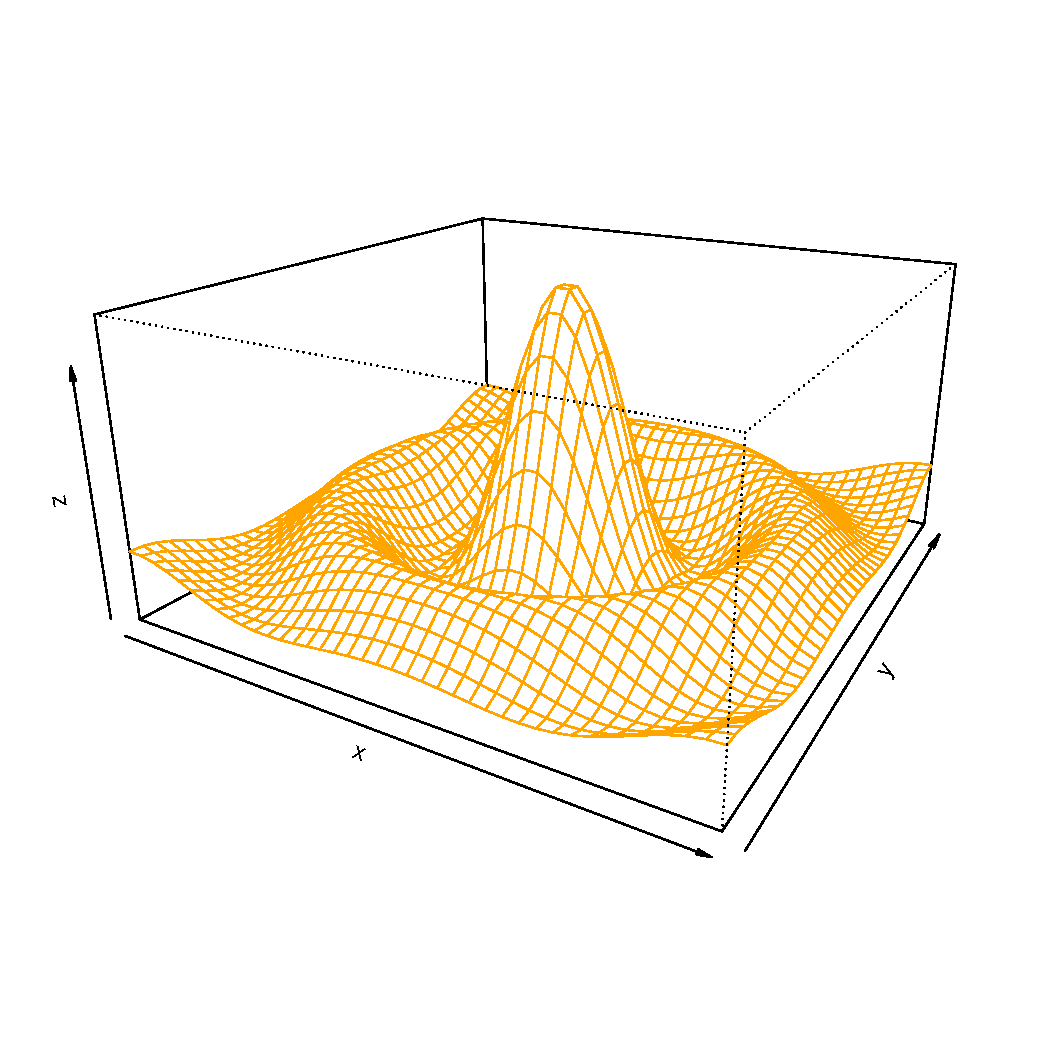
\includegraphics[height = 7.5cm, width = 7.5cm]{figure/Lighting_1.pdf}
		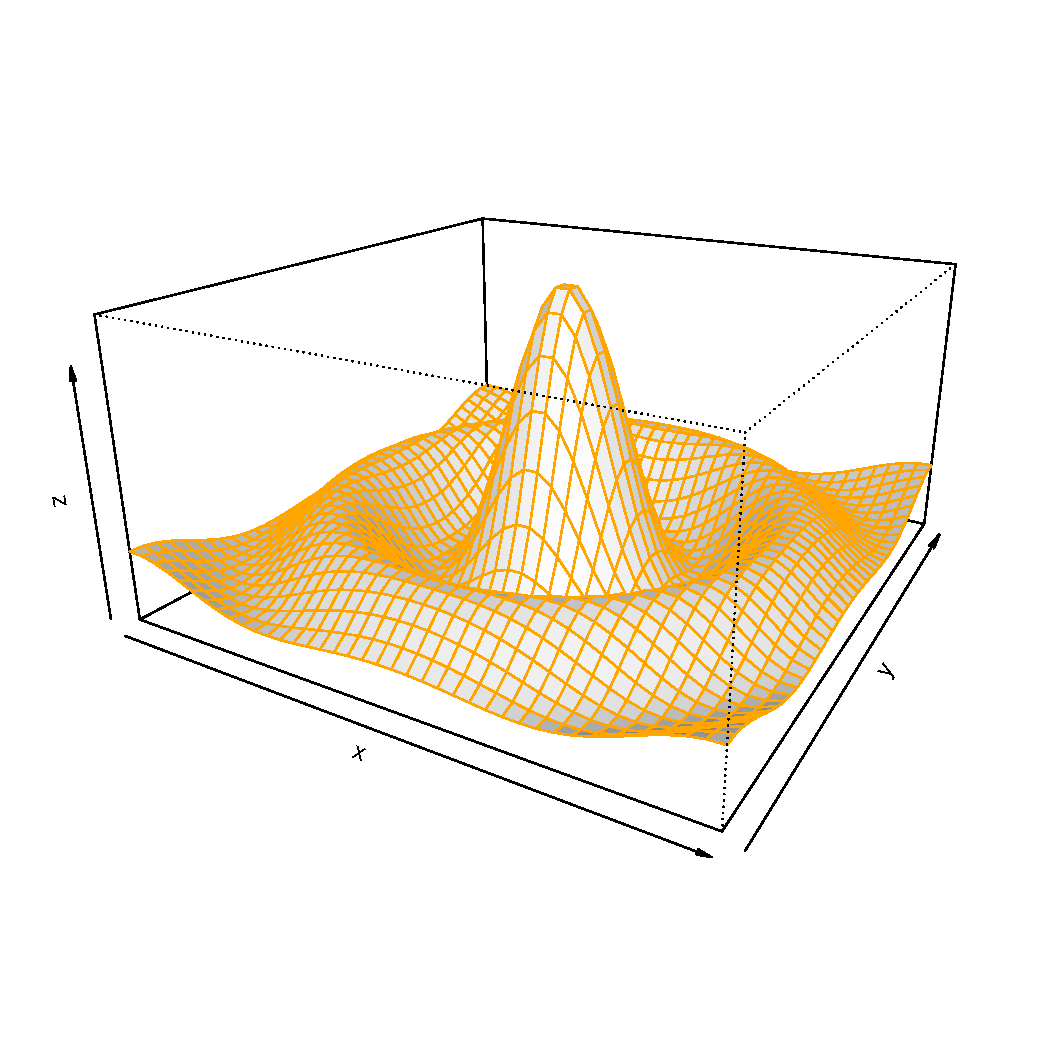
\includegraphics[height = 7.5cm, width = 7.5cm]{figure/Lighting_2.pdf}
		\caption{Adding a light source to the perspective plot from the same angel of view. The left plot is origin plot without shading, where the right plot is being shaded.}
		\label{figure_3.3}
	\end{center}
\end{figure}

\newpage
\subsection{Difference between \texttt{C} and \texttt{R}}
There are many functions in \texttt{R} call \texttt{C} code to do a lot of the work. Although the structure of \texttt{C} code is similar to \texttt{R} code in some special cases, there are some \texttt{C} code structures which behave completely different to \texttt{R}, therefore translating \texttt{C} code to \texttt{R} code is not as simple as "copy-and-paste".\\

\subsubsection{Pointers}
One main data structure in \texttt{C} is the pointer, which is a type of reference that records the address/location of a global object or a local variable in a function. Pointers can be manipulated by using assignment or pointer arithmetic.
\begin{lstlisting}[language = C]
static int LimitCheck(double *lim, double *c, double *s)
{
    if (!R_FINITE(lim[0]) || !R_FINITE(lim[1]) || lim[0] >= lim[1])
    return 0;
    *s = 0.5 * fabs(lim[1] - lim[0]);
    *c = 0.5 * (lim[1] + lim[0]);
    return 1;
}
\end{lstlisting}

The top piece of code is used for checking the Limit for the \texttt{persp()} function. It also multiplying the variable \textttt{c} and \texttt{s} for further calculation. In this case, the \texttt{c*} and \texttt{s*} are the pointer which will point to the machine memory of \texttt{s} and \texttt{c} and modify them.\\

However, this process cannot be reproduced on \texttt{R} because \texttt{R} does not have the pointer data structure. One possible solution will be rather than doing the Limit checking and multiply \texttt{s} and \texttt{c}, do the limit checking and return/assign the \texttt{s} and \texttt{c} as \texttt{xs} ad \texttt{ys} for further calculation.
\begin{lstlisting}[language = R]
LimitCheck = function (lim){
    s = 0.5 * abs(lim[2] - lim[1])
    c = 0.5 * (lim[2] + lim[1])
    c(s, c)
}
xs = LimitCheck(xr)[1]
xc = LimitCheck(xr)[2]
...
\end{lstlisting}

\newpage
\subsubsection{Array}
The other main difference is that \texttt{C} uses array data format but \texttt{R} uses matrix data format. 
\begin{lstlisting}
FindPolygonVertices(c[k - 1], c[k],
                    x[i - 1], x[i],
                    y[j - 1], y[j],
                    z[i - 1 + (j - 1) * nx],
                    z[i + (j - 1) * nx],
                    z[i - 1 + j * nx],
                    z[i + j * nx],
                    px, py, pz, &npt);


out = lFindPolygonVertices(sc[k], sc[k + 1],
                          x[i], x[i + 1],
                          y[j], y[j + 1],
                          z[i, j],
                          z[i + 1, j],
                          z[i, j + 1],
                          z[i + 1, j + 1],
                          px, py, pz, npt)
\end{lstlisting}



To get the same elements in the matrix as the elements in the array, one solution is to change the matrix data format into vector data format. However, \texttt{R} is familiar with matrix data structure. Hence it is easier and more understandable by \texttt{R} user and programmer. The \texttt{z[i - 1 + (j - 1) * nx]} in \textt{FindPolygonVertices()} is selecting the $i^{th}$ element from the $j^{th}$ column, which the following \texttt{R} code provide the same result That is, \texttt{z[i, j]} in \texttt{R} will provide the same result as \texttt{C} \\

However, the \texttt{z} is array in the first call as it written on \texttt{C} but the second is matrix as it written on \texttt{R}. the - 1 on the \texttt{R} code because \texttt{C} starting at 0 index but \texttt{R} starting at 1.\\

\subsection{Box and other features}
One feather that \texttt{persp()} supported is whether or not to draw a container (box) around the surface. (See Figure \ref{figure_3.4}). Therefore, it is necessary to find out whether the edge of the box in front of the surface or behind the surface. \\ 

The solution will be that translates the \texttt{C} code to \texttt{R} code directly. The reason for doing this directly translation is that R is sensitive on drawing the dot lines. More specifically, it may cause difference if we connect two points with a dotted line in different direction. Due to the purpose of this paper, the plot should be drawn as identical as possible. Therefore, the direct translation is required.\\


\begin{figure}[h]
	\begin{center}
		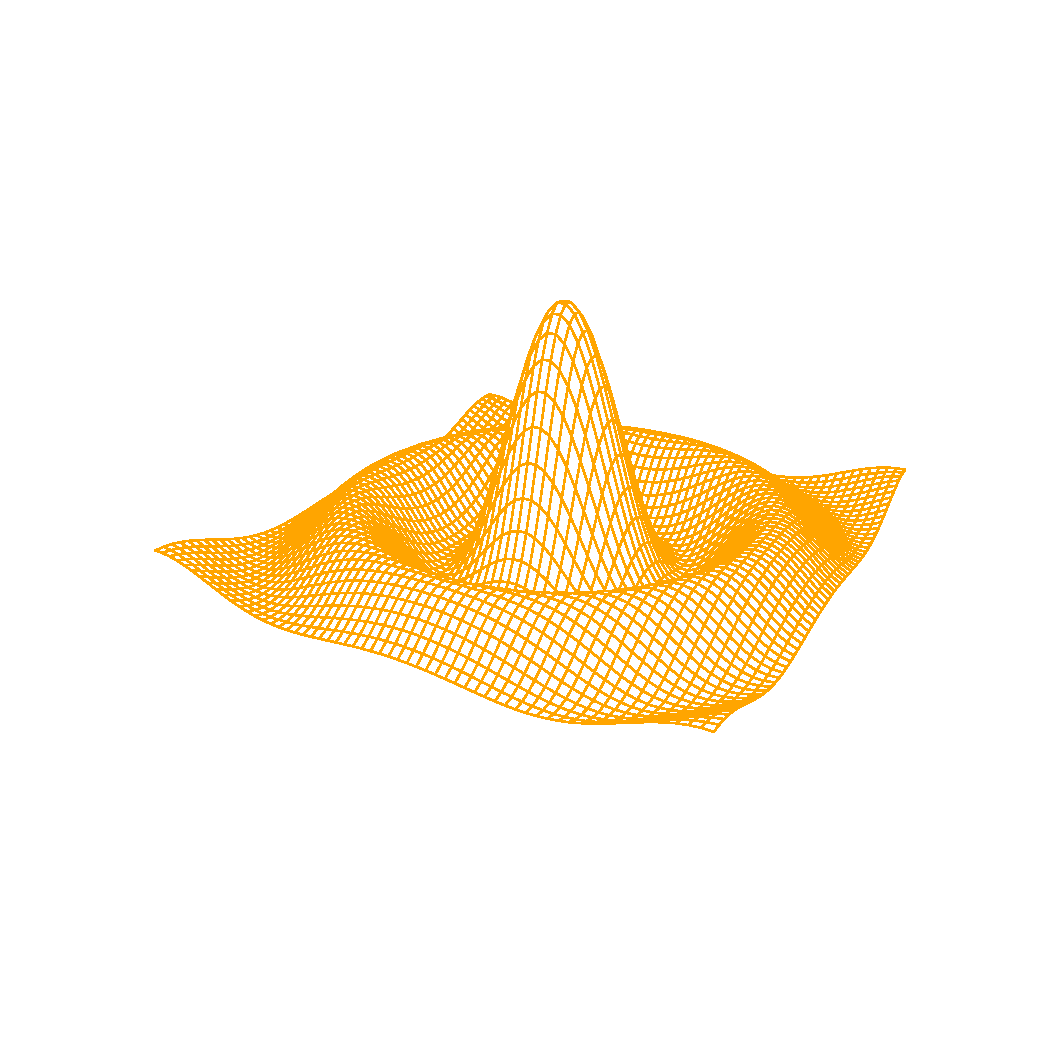
\includegraphics[height = 7.5cm, width = 7.5cm]{figure/box_example_1.pdf}
		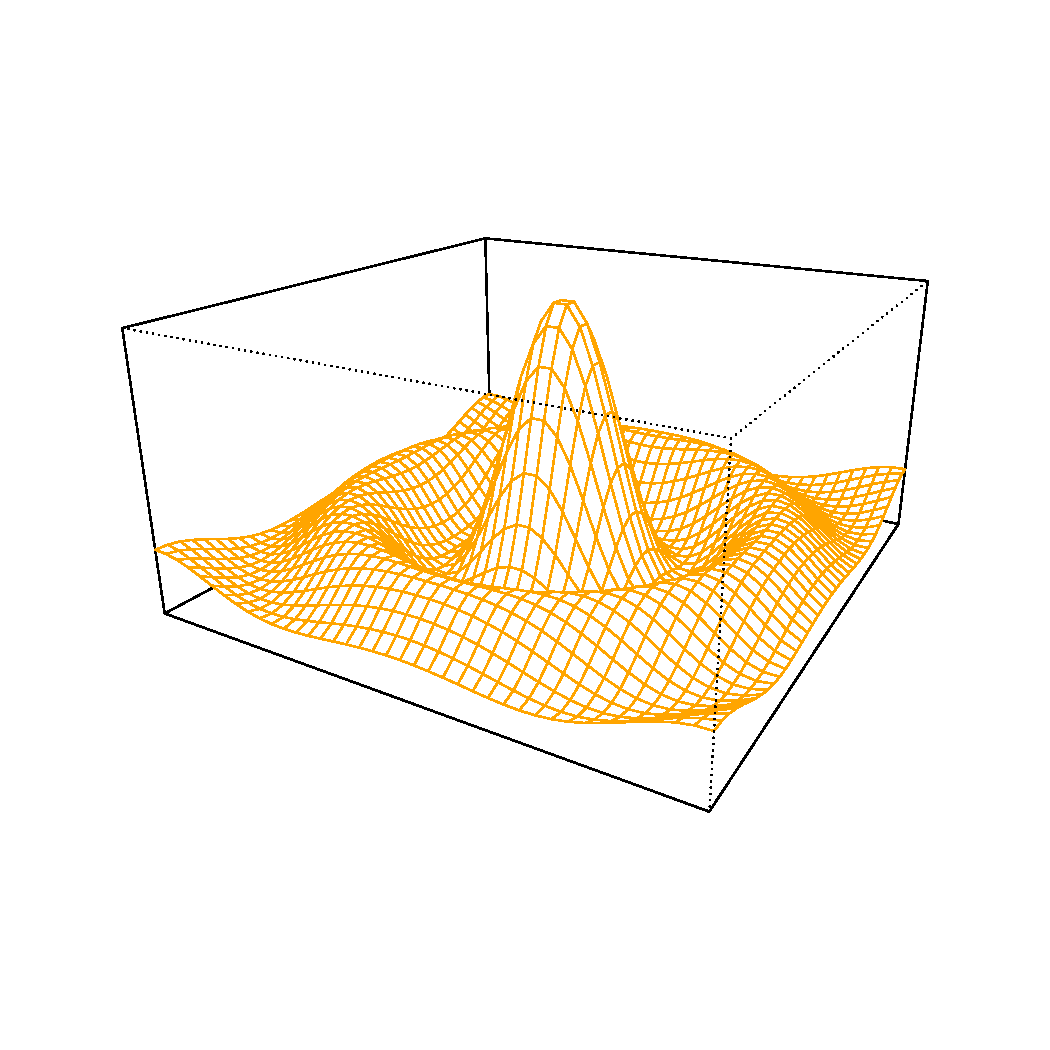
\includegraphics[height = 7.5cm, width = 7.5cm]{figure/box_example_2.pdf}
		\caption{The surface been drawn by ignore the box in the left plot, right plot drawn the surface as well as box}
		\label{figure_3.4}
	\end{center}
\end{figure}

Other feather that \texttt{persp} supported is the detail of the axis. (See Figure \ref{figure_3.5}). The axis has three type, no axes, simple axes which only contain the label of axes, or showing the scale of each axes. These feathers are required to be reproduced by \textbf{grid}, The solution to this problem by translating the \texttt{C} code to \texttt{R} code directly.



\begin{figure}[h]
	\begin{center}
		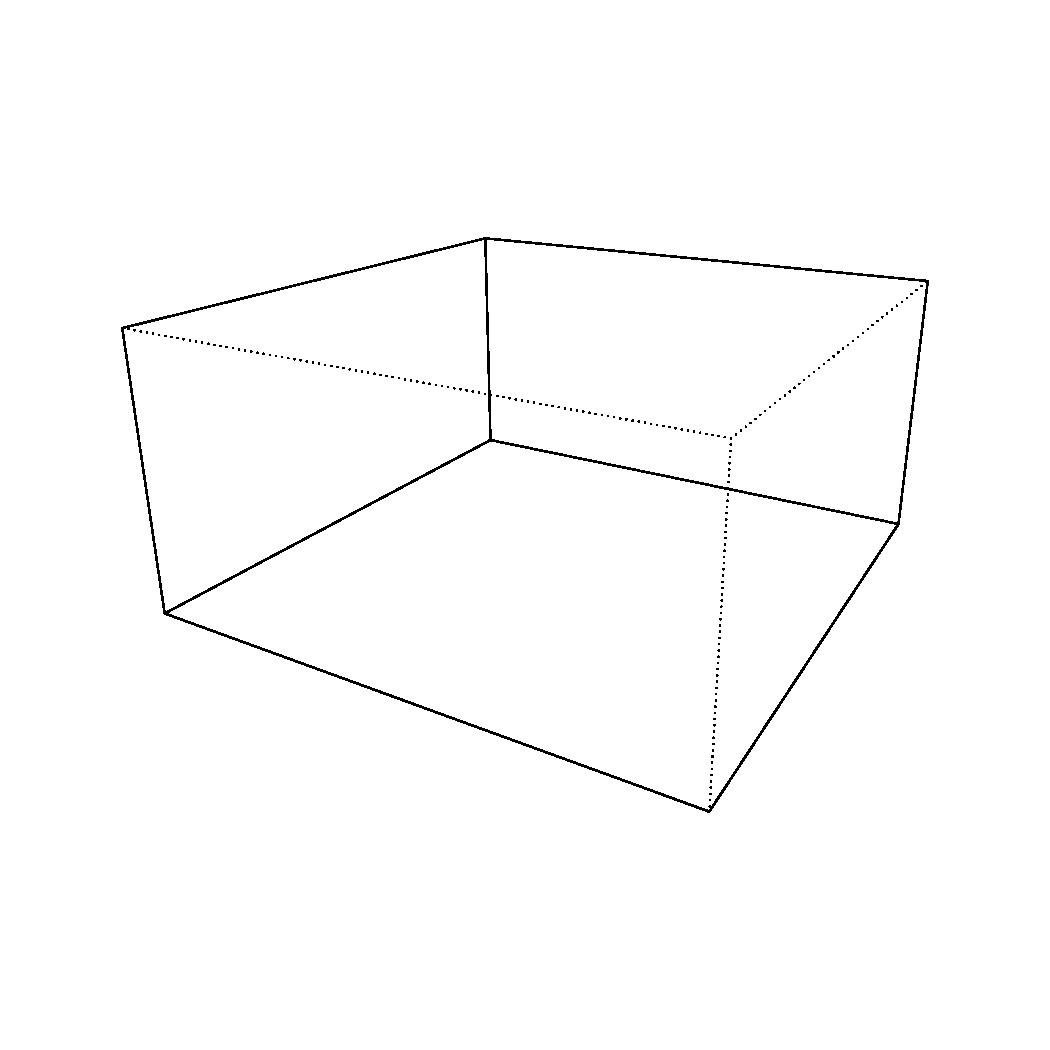
\includegraphics[height = 5cm, width = 5cm]{figure/axis_example_1.pdf}
		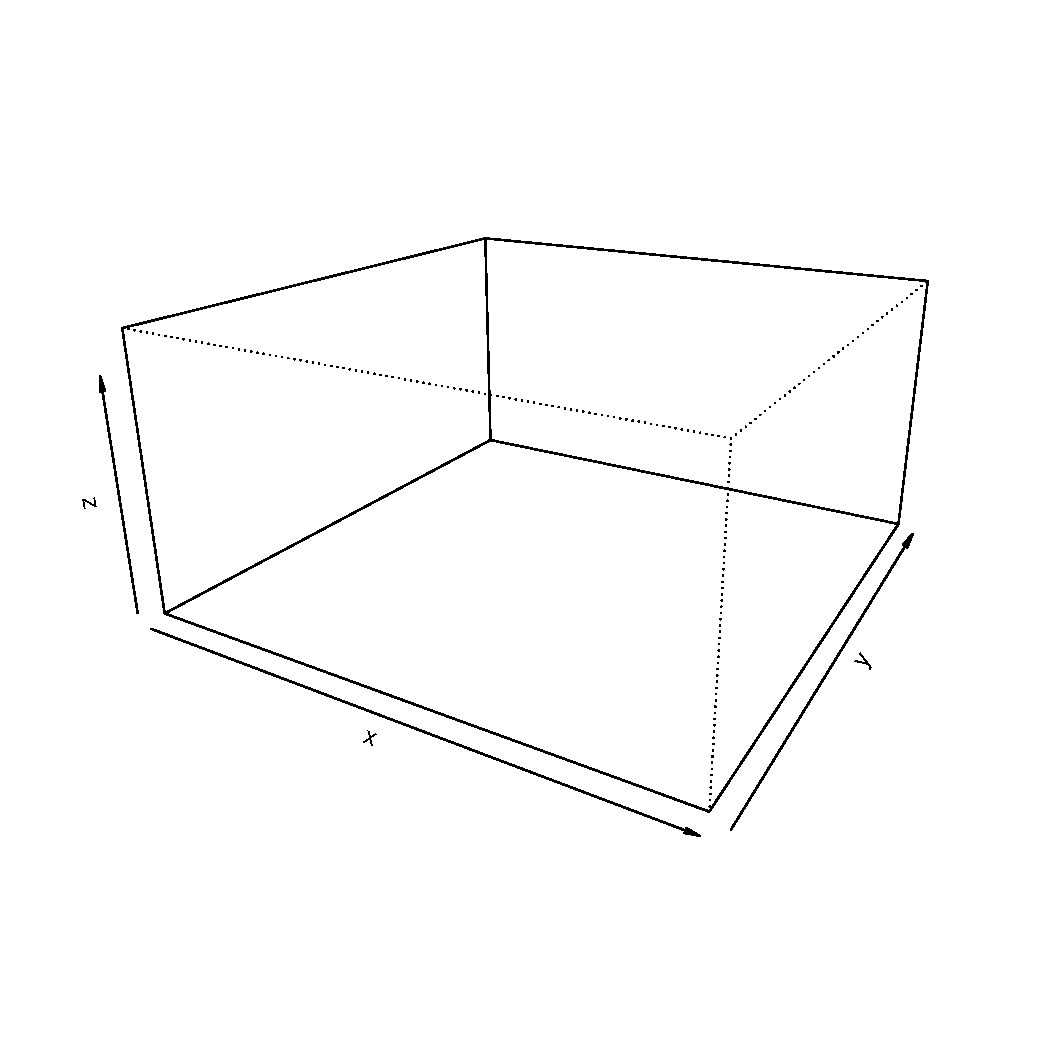
\includegraphics[height = 5cm, width = 5cm]{figure/axis_example_2.pdf}
		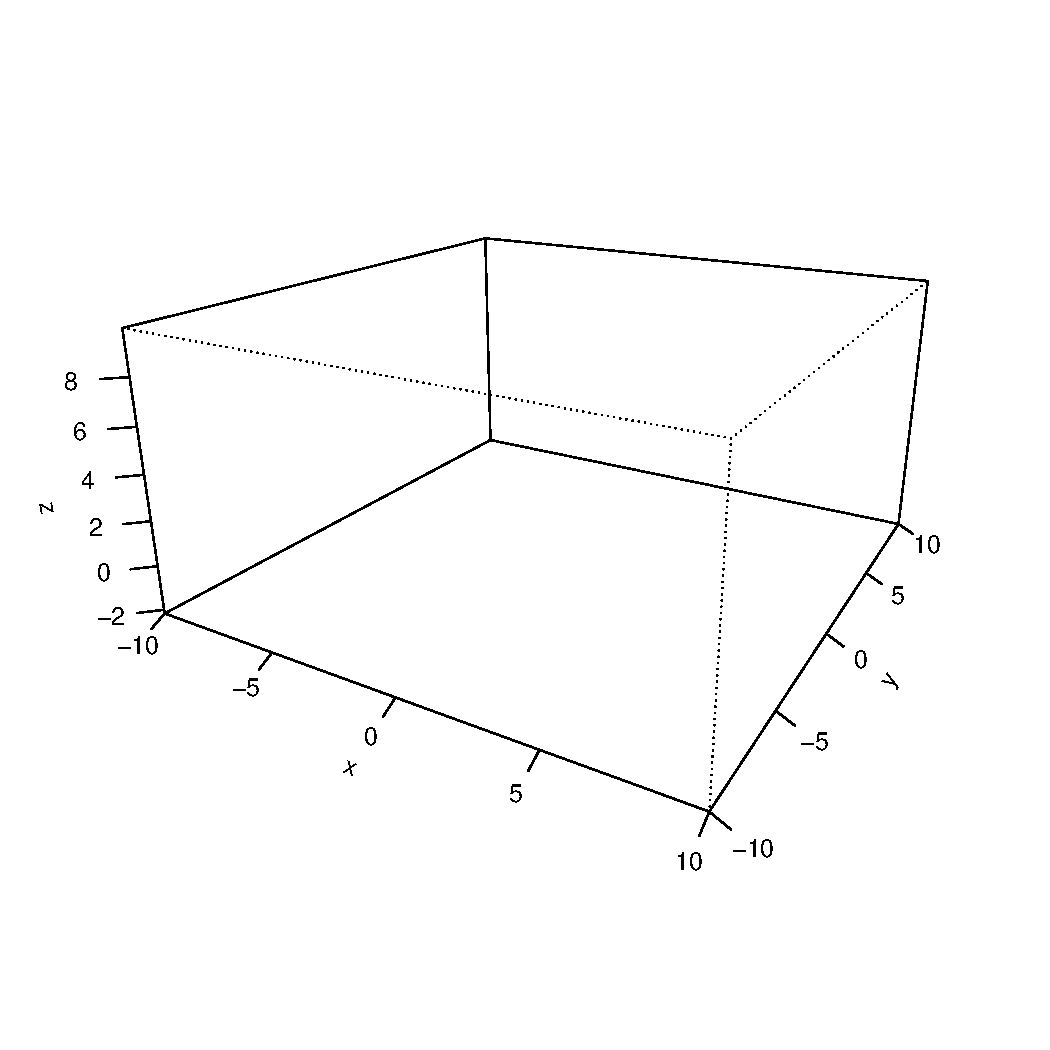
\includegraphics[height = 5cm, width = 5cm]{figure/axis_example_3.pdf}
		\caption{The Perspective surfaces are being ignored in this example, the left plot shows no axis been drawn, the simple axes been drawn in the middle plot and the right plot shows more detail for each axis.}
		\label{figure_3.5}
	\end{center}
\end{figure}

\section{The Filled Contour Plot}
\subsection{Direct translation from \texttt{C} to \texttt{R}}
The other tasks of this paper is to emulate the Level (Contour) Plots (\texttt{filled.contour}) from \textbf{graphics} to \textbf{grid}. Similar to \texttt{persp()}, the first step to emulate \texttt{filled.contour} is to access the information from the graphics engine display list. (See Figure \ref{figure_3.6})
\begin{Schunk}
\begin{Sinput}
> x = 10*1:nrow(volcano)
> y = 10*1:ncol(volcano)
> filled.contour(x, y, volcano, color = terrain.colors,
+               plot.title = title(main = "The Topography of Maunga Whau",
+               xlab = "Meters North", ylab = "Meters West"),
+               plot.axes = { axis(1, seq(100, 800, by = 100))
+               axis(2, seq(100, 600, by = 100)) },
+               key.title = title(main = "Height\n(meters)"),
+               key.axes = axis(4, seq(90, 190, by = 10)))
> xx = recordPlot()
> info = xx[[1]][[12]][[2]]
> head(info[[2]])  ## print the values of x
\end{Sinput}
\begin{Soutput}
[1] 10 20 30 40 50 60
\end{Soutput}
\begin{Sinput}
> head(info[[3]])  ## print the values of y
\end{Sinput}
\begin{Soutput}
[1] 10 20 30 40 50 60
\end{Soutput}
\begin{Sinput}
> dim(info[[4]])  ## print the dimension of z
\end{Sinput}
\begin{Soutput}
[1] 87 61
\end{Soutput}
\begin{Sinput}
> length(info[[5]])  ## print the length of s
\end{Sinput}
\begin{Soutput}
[1] 22
\end{Soutput}
\end{Schunk}
\begin{figure}[h]
	\begin{center}
		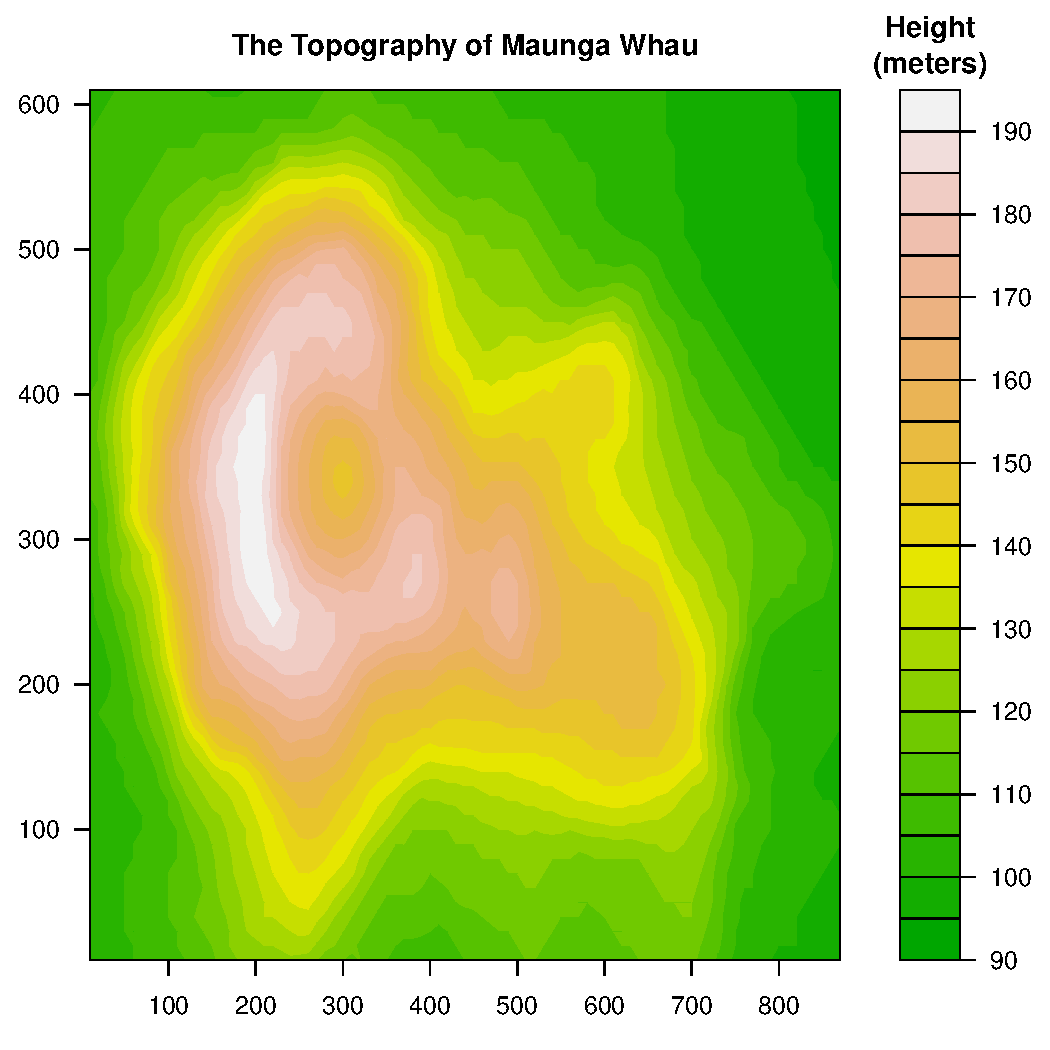
\includegraphics[height = 10cm, width = 12cm]{figure/filled_example_1.pdf}
		\caption{The topography of the Maunga Whau been drawn by using the \texttt{filled.contour}}
		\label{figure_3.6}
	\end{center}
\end{figure}
The example shows the plot of topography of Maunga Whau and also the information from the \texttt{filled.contour} call in the graphics engine display list. Same problem as \texttt{persp()}, there is no way to reproduce this plot directly by only using the inputs from the \texttt{filled.contour()}.\\

There is an algorithm to create this contour plot in the \textbf{graphics} package written by \texttt{C}. The first step of the solution will be translated the \texttt{C} code directly to maximize the accuracy.\\

\begin{lstlisting}[language = C]
static void
FindPolygonVertices(..., double *x, double *y, double *z, int *npt, ...)
{
    *npt = 0;
    FindCutPoints(low, high, x1,  y1,  z11, x2,  y1,  z21, x, y, z, npt);
    FindCutPoints(low, high, y1,  x2,  z21, y2,  x2,  z22, y, x, z, npt);
    FindCutPoints(low, high, x2,  y2,  z22, x1,  y2,  z12, x, y, z, npt);
    FindCutPoints(low, high, y2,  x1,  z12, y1,  x1,  z11, y, x, z, npt);
}
\end{lstlisting}
This piece of \texttt{C} code is the algorithm used for calculate the coordinates of the vertex of each polygon in the level contour plot. The parameters \textbf{*x}, \textbf{*y}, \textbf{*z} are the array pointers which have length of 8, individually, \textbf{*npc} is also a pointer has length of 1. If the \texttt{FindCutPoints()} is called, the elements in the arrays of \textbf{x}, \textbf{y}, \textbf{z} will be modified. In general, we feed the location of memory of \textbf{x}, \textbf{y}, \textbf{z} and \textbf{npt} to \texttt{FindPolygonVertices()} and modify the values of \textbf{x}, \textbf{y}, \textbf{z} and \textbf{npt} inside the \texttt{FindCutPoints()}.\\

For example, the first call of \texttt{FindCutPoints()} modifies the elements in the pointer arrays of $x$, $y$, $z$. The location of elements in arrays been modified will depend on the parameter $*npt$. More specifically, the $x$ as a function of $x_1$ and $x_2$, $y$ as a function of $y_1$ and so on. The second \texttt{FindCutPoints()} is slightly different, $x$ will depend on a function of $x_2$, $y$ as a function of $y_1$ and $y_2$. In the third \texttt{FindCutPoints()} call, $x$ will depend on a function of $x_2$ and $x_1$, $y$ will depend on a function of $y_2$. Finally, $x$ will depend on a function of $x_1$, $y$ depend on the function of $y_2$ and $y_1$. \\

There is no pointer data structure in \texttt{R} hence we cannot produce the same action as \texttt{C}. One approximation to this action will be as follows:
\begin{lstlisting}[language = R]
lFindPolygonVertices = function(...)
{
    out = list(); npt = 0
    out1 = lFindCutPoints(...)
    x = y = z = numeric(8); npt = out1$npt

    out$x = out1$x + out2$y + out3$x + out4$y
    out$y = out1$y + out2$x + out3$y + out4$x
    out$npt = out4$npt
    out
}
\end{lstlisting}
Instead of mortify $x$, $y$, $z$ and $npt$ inside \texttt{FindCutPoints()}, record the values for $x$, $y$, $z$ and $npt$ outside the \texttt{lFindCutPoints()} call in \texttt{R} every time. At last, we combined every $x$ and $y$ together as the previous \texttt{C} code behave. 


\subsection{Vectorization}
In \texttt{C}, the total iteration in the loops is equal to
\begin{equation}
Total = nx * ny * ns
\end{equation}
Where:\\
\textbf{nx = length(x) - 1}\\
\textbf{ny = length(y) - 1}\\
\textbf{ns = length(levels) - 1}\\

It requires huge iteration. For example, In Figure \ref{figure_3.6}, the Topography of Maunga Whau, the length of x is 87 and the length of y is 61, where the length of levels is 22. Therefore, there are at most 108360 polygons that we need to consider which it will slow down the software. Instead of calculate the coordinates of every polygons one by one, it is a good idea to vectorize the function to speed up the software.

\begin{Schunk}
\begin{Sinput}
> ## time comparison
> filled.contour.volcano()
> ## time for loop version of fille.contour()
> system.time(grid.echo())
> # user  system elapsed 
> # 10.03    0.23   10.32 
> 
> ## time for for vectorizetion version of fille.contour()
> system.time(grid.echo())
> # user  system elapsed 
> # 1.28    0.53    1.82 
\end{Sinput}
\end{Schunk}


	The previous code is testing the efficiency of the methods by using \texttt{system.time()}. First of all, we draw the filled contour plot for the Topography of Maunga Whau, then we tried to redraw it in \textbf{grid} by using two different implement methods. One is the directed translation from \texttt{C} by using multiple loops (old method) and the other one is using vectorization (new method).\\
	The result shows that the new method (1.82 seconds) is much faster than the old method (10.32 seconds).

\chapter{Integrate to \textbf{gridGraphics} package}
\section{Some concept of \textbf{grid}}
The previous section explained the internal calculation for \texttt{persp()} and \texttt{filled.contour()}. It works perfectly outside the \textbf{gridGraphics} package. However, \texttt{grid.echo()} still cannot emulate these two kinds of plot because they are not been integrated to the package yet. Therefore, it requires more work.\\ 

The \textbf{gridGraphics} package provides the structure of viewports which act identical to the layout of plots in the plot region been drawn by \textbf{gridGraphics}. 

\begin{Schunk}
\begin{Sinput}
> set.seed(110)
> par(mfrow = c(1,2))
> x = rnorm(1000)
> hist(x, probability = T)
> plot(density(x))
> grid.echo()
\end{Sinput}
\end{Schunk}
\begin{figure}[h]
	\begin{center}
		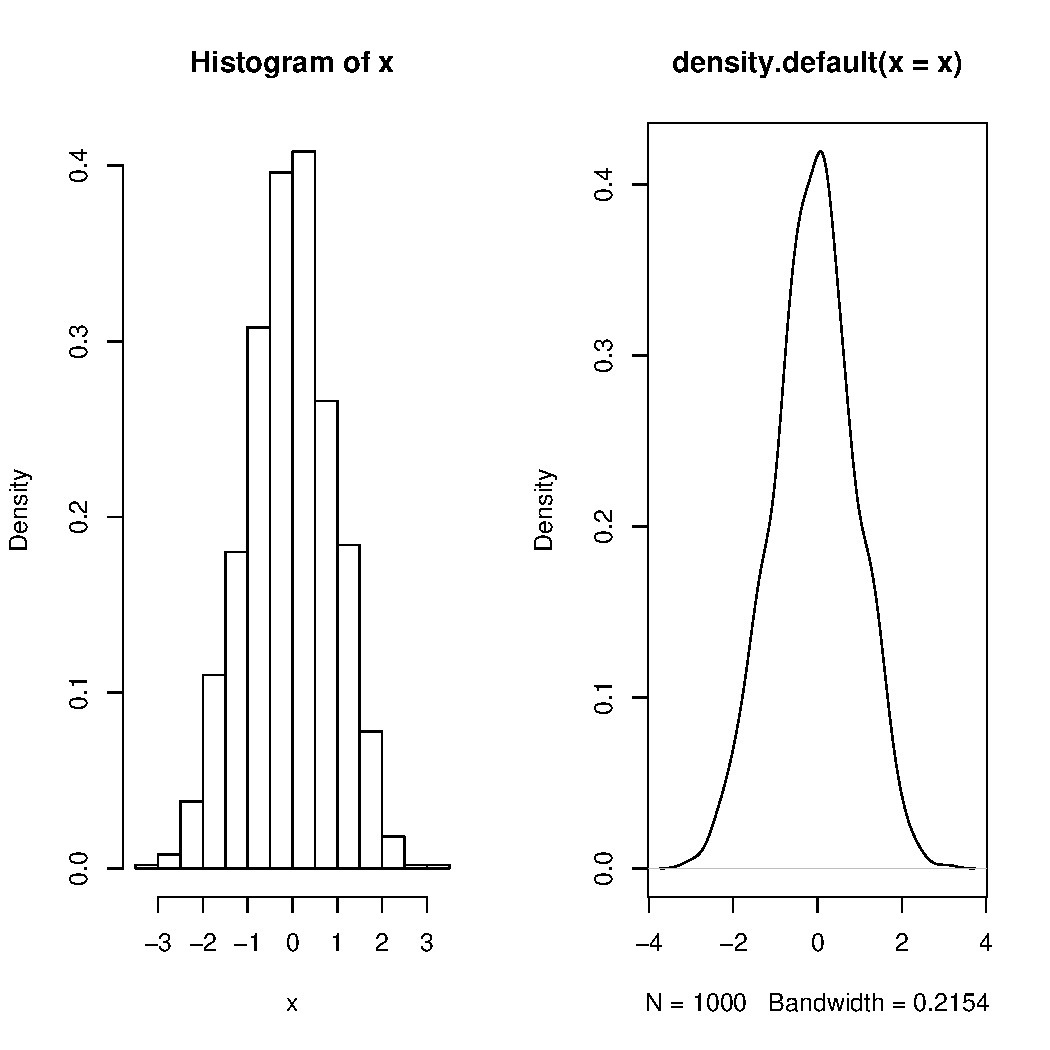
\includegraphics[height = 8.5cm, width = 15cm]{figure/viewport_demo_1.pdf}
		\caption{display the \textbf{grid} version of draw two plots into one overall graph by setting \texttt{par(mfrow())}. The left-plot is the histogram of observations generated by standard normal distribution, right-plot is the density plot of the observations}
		\label{figure_4.1}
	\end{center}
\end{figure}

\begin{lstlisting}[language = R]
grid.ls(viewports = TRUE)

graphics-root
  graphics-inner
    graphics-figure-1
      graphics-plot-1-clip
        graphics-window-1-1
          graphics-plot-1-rect-1

graphics-root
  graphics-inner
    graphics-figure-2
      graphics-plot-2-clip
        graphics-window-2-1
          graphics-plot-2-lines-1


\end{lstlisting}
% PerspWindow, 
The previous code used the \textbf{graphics} package to plot a histogram on the left and a density plot of one thousand random observations generated by standard normal distribution. Then redraw the plot on \textbf{grid}. (See Figure \ref{figure_4.1}.) The grobs object and the veiwports are created. \\

The grobs object and the veiwports and been listed by \texttt{grid.ls()}. In the previous example, we can see that the contents(rectangles) of histogram were drawn in the viewports of \texttt{graphics-inner::graphics-figure-1::graphics-plot-1-clip::graphics-window-1-1}. The density plot was drawn in the other viewports which is \texttt{graphics-inner::graphics-figure-2::graphics-plot-2-clip::graphics-window-2-1}. Although it is completely different structure of the plot that was drawn by \textbf{graphics}, they are identical to each other.\\

To reproduce the same plots as \textbf{graphics}, we need to modify the \textbf{grid} structure of the plot so that it behaves identically to the plot that was drawn by \textbf{graphics}. In this example, the viewports need to be set in the same location and the same size as the \textbf{graphics} plot region, and, the x-scale and y-scale of the viewports in \textbf{grid} need to be set the same user coordinates as in \textbf{graphics}.\\

\section{Integrate \texttt{persp()}}
The core of \textbf{gridGraphics} package provides some basic viewport structure to support the perspective plots(\texttt{persp()}), based on the general plots that been drawn by \textbf{graphics}. However, there are some specific details that \textbf{gridGraphics} not fully supported.
The following problems need to be solved before integrating \texttt{persp()} into the package:
\begin{itemize}
	\item{The scaling of the viewport needs to be calculated}
	\item{Determine whether the clipping happens for every component when drawing}
\end{itemize}

It is not allowable to create a new viewport structures starting with \texttt{grid.newpage()}, which creates a new grid page because it will rest the viewport structures, even it will reset the viewports that created by \texttt{gridGraphics}
For example, the points and lines added to perspective plot. These features will disappear when calling \texttt{grid.echo()}, because \texttt{grid.newpage()} will clean all the contents and structures in the current graphics devices. Therefore, it is necessary to draw the perspective plot in the correct viewport, which under the structure provided by \textbf{gridGraphics}.\\

The other problem that we may consider is the actual scale for the viewport, i.e. the x-scale and y-scale. Unfortunately, \textbf{gridGraphics} does no support the calculation for the actual limit of x and y since the other kinds of plot that \textbf{graphics} provides is in two dimension. The calculation of the limit of x and y is not as simple as \texttt{range(x)} or \texttt{range(y)}, because we are mapping a 3-dimensions objects into the 2-dimension graphics device, therefore the limit of x and y in the graphics device is not equal the limit of x and y of the origin 3-dimension object.\\

The final problem will be whether the clipping happened. More specifically, the different components of the perspective plot should be drawn in clipped region or non-clipped region.\\

The limit of x and y will depend on the ratio of horizontal and vertical length of the current windows graphics devices. On \textbf{grid}, it is simple to track the actual length of the viewport in the current windows graphics devices. \\

The following example is calculating the vertical length and horizontal length of the viewport in current windows graphics devices. (See Figure \ref{figure_4.2}) The dotted rectangle region is the viewport region that we focus on. As result, the vertical length of the viewport in current windows graphics devices in my PC is 5.16 inches, where the horizontal length is 5.76 inches. \\
\begin{Schunk}
\begin{Sinput}
> plot(cars$speed, cars$dist, col = 'orange', 
+       pch = 16, xlab = 'speed', ylab = 'dist')
> grid.echo()
> downViewport('graphics-plot-1')
> grid.rect(gp = gpar(col = 'red', lty = 12221, lwd = 2))
> convertX(unit(1.0, 'npc'), 'inches')
\end{Sinput}
\begin{Soutput}
[1] 5.76inches
\end{Soutput}
\begin{Sinput}
> convertY(unit(1.0, 'npc'), 'inches')
\end{Sinput}
\begin{Soutput}
[1] 5.16inches
\end{Soutput}
\end{Schunk}

\begin{figure}[h]
	\begin{center}
		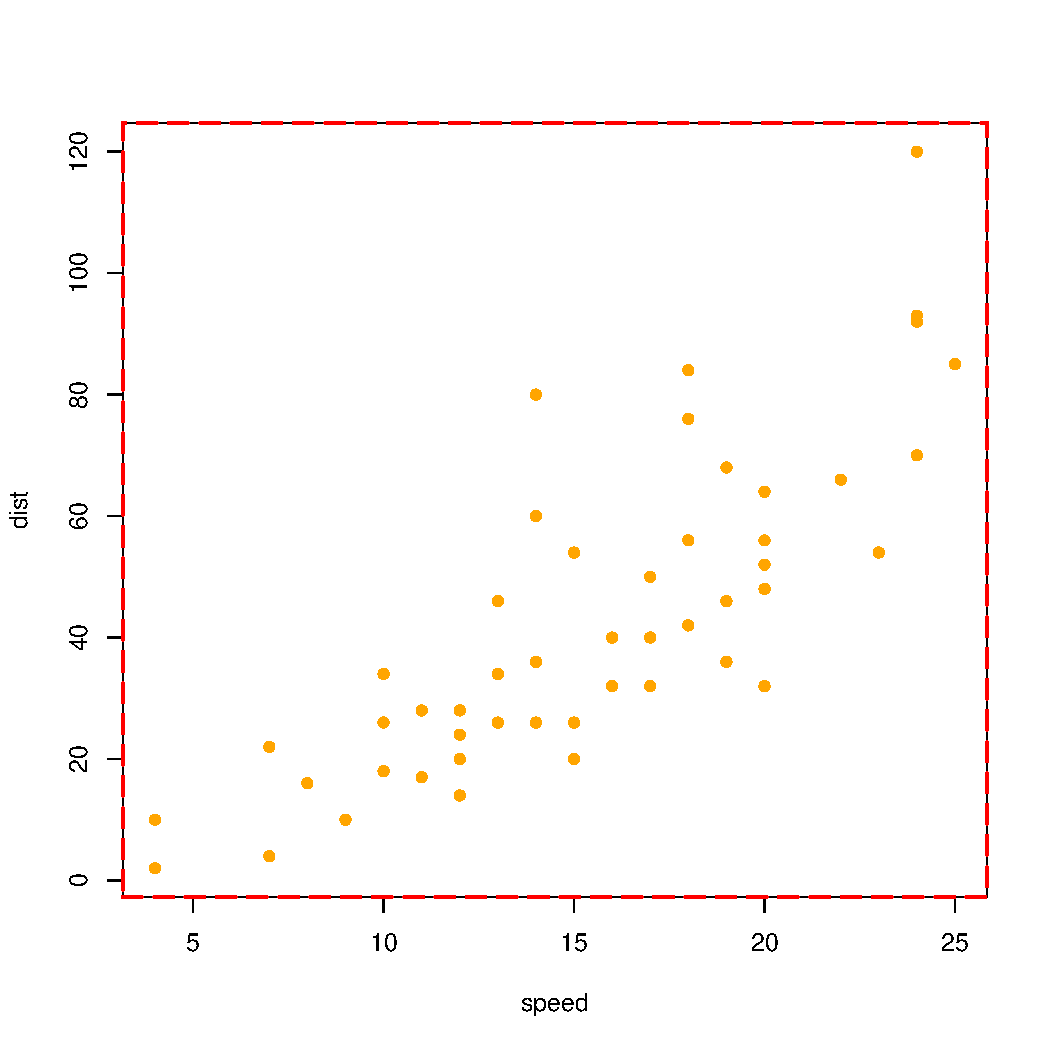
\includegraphics[height = 8cm, width = 8cm]{figure/gridGraphics_persp_demo_1.pdf}
		\caption{Used the example from chapter 2, calculate the actual vertical length and horizontal length of the viewport (the region of the red dotted line)}
		\label{figure_4.2}
	\end{center}
\end{figure}

\newpage
The idea of this example is that it is possible to track the actual vertical length and horizontal length by navigating to the specific viewport and record them. It leads to the solution of our second problem, first of all, we navigate to the viewport that has been drawn by \texttt{persp()}, calculate the limit of x and y base on the size of this viewport. Then we create another viewport (visible for other \textbf{gridGraphics} functions e.g. \texttt{lines()} and \texttt{points()}) that has the same location and the same size as the previous viewport. Then we modify the x-scale and y-scale from the new viewport to be the limit of x and y that we calculated. Finally, the concepts of \texttt{persp()} will be drawn in this viewport. \\

\begin{lstlisting}[language = R]
testPersp21(box = FALSE)
usr = par('usr')
rect(usr[1], usr[3], usr[2], usr[4], lty = 12221, lwd = 2, border = 'red')
usr
## [1] -0.4555925  0.3807924 -0.5003499  0.3360350
grid.echo()
downViewport('graphics-window-1-0'); 
grid.rect(gp = gpar(col = 'red', lty = 12221))
c(current.viewport()$xscale, current.viewport()$yscale)
## [1] -0.04  1.04 -0.04  1.04
\end{lstlisting}

\begin{figure}[h]
	\begin{center}
		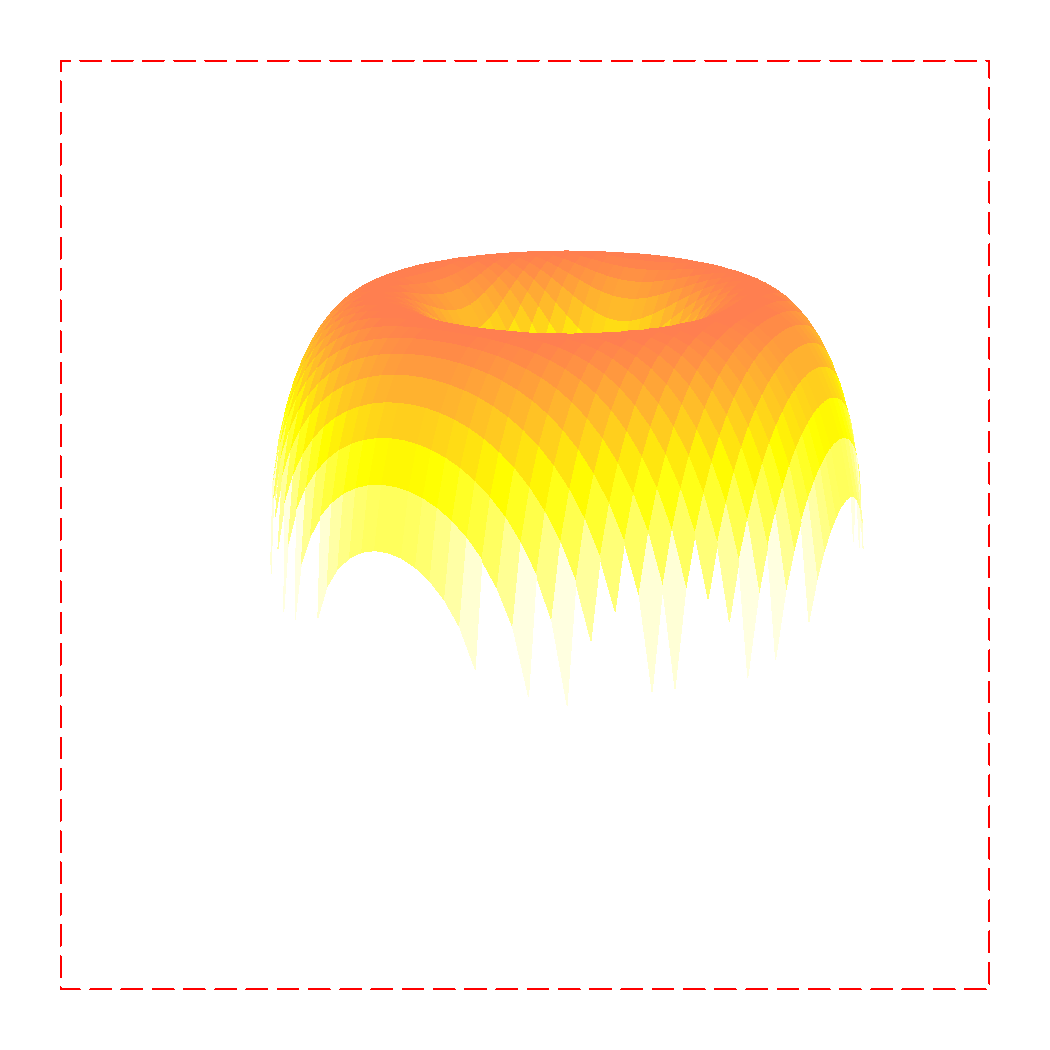
\includegraphics[height = 7cm, width = 7cm]{figure/gridGraphics_persp_demo_viewport_1.pdf}
		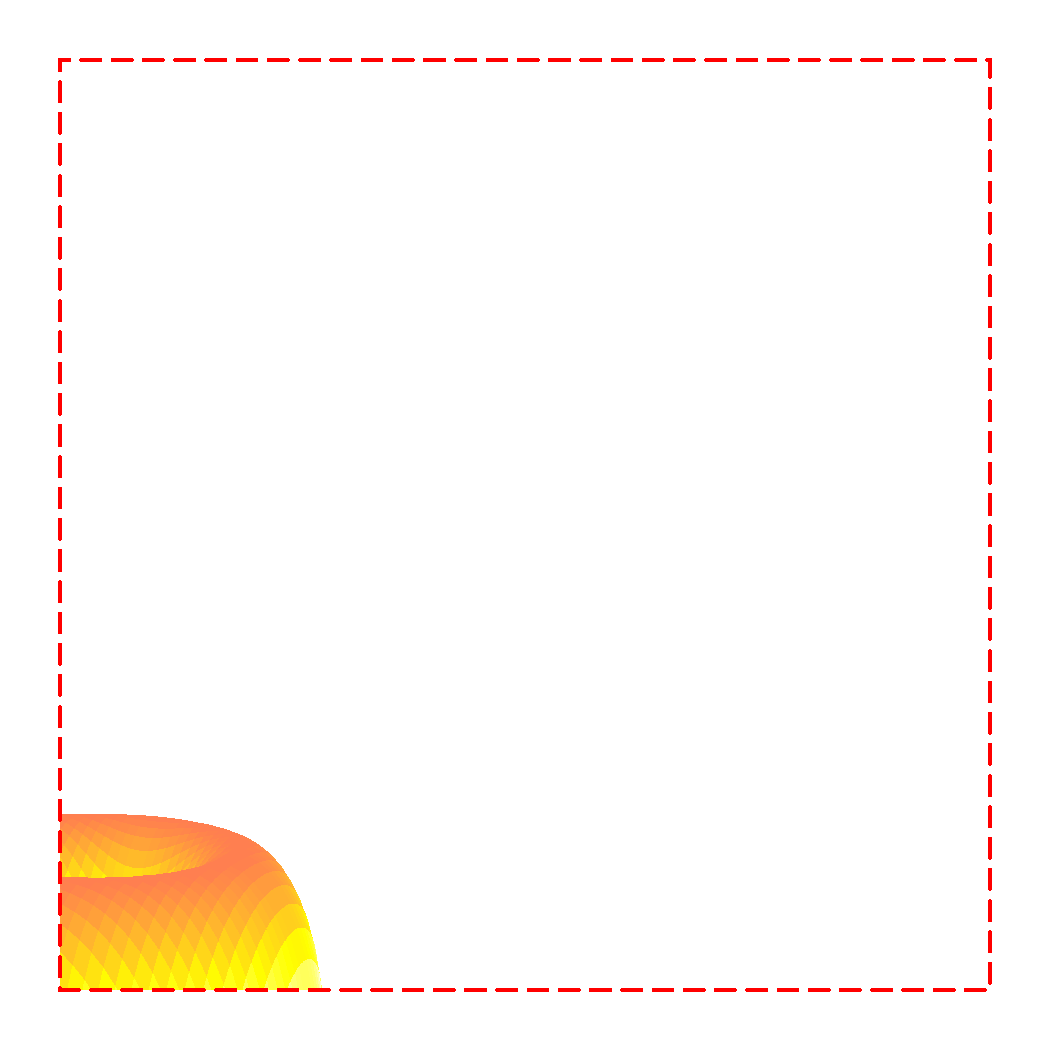
\includegraphics[height = 7cm, width = 7cm]{figure/gridGraphics_persp_demo_viewport_2.pdf}
		\caption{A Torus been drawn by \texttt{persp()} on the left plot, the right plot tried to reproduce the \texttt{persp()}, because of the scale of the viewport is different to the limit, the Torus is been drawn on the bottom-left corner.}
		\label{figure_4.3}
	\end{center}
\end{figure}

Figure \ref{figure_4.3} shows a Torus drawn on the plot region. The red dotted rectangles indicate the plot region of \textbf{graphics}(left plot) and the viewport region for \textbf{grid}(right plot). Although the plot region is identical to the viewport region, the scales are different. The limit of x and y are $(-0.4555925,  0.3807924)$, $(-0.5003499,  0.3360350)$. The scale of x and y in the viewport region are $(-0.04,  1.04)$, $(-0.04,  1.04)$. Therefore, the scale needs to be modified. \\

\newpage
\begin{lstlisting}[language = R]
## navigate to the viewport
depth = gotovp(TRUE) 
## calculate the limit of x and y
lim = PerspWindow(xr, yr, zr, trans, 'r')
## lim = -0.4555925 0.3807924 -0.5003499 0.3360350
## create another viewport by using the limit that we just calculated
vp = viewport(0.5, 0.5, 1, 1, default.units = 'npc',
              xscale = lim[1:2], yscale = lim[3:4]) 
## back to the Root viewport
upViewport(depth)  
\end{lstlisting}
The previous code is creating a new temporary viewport which contains the true x-scale and y-scale prepared for drawing the perspective plot. The values for x scale and y scale are calculated by \texttt{PerspWindow()}. It will do the calculation by considering the 'actual' ratio of horizontal length and vertical length of the current graphics device, similar to the calculation of the \texttt{C} code does.\\
After we create the temporary viewport that contains the correct scale, then we added this viewport to the location of the tree which inside the viewport created by \textbf{gridGraphics}. That is, push temporary viewport inside the odd viewport. The Final step will be drawn the concepts within this viewport. To do that, we need to push a temporary viewport every time we drawn. The following code is how does the surface of the plot is drawn internally.

\begin{lstlisting}[language = R]
## navigate to the viewport which has the true limit of x and y
depth = gotovp(FALSE)
pushViewport(vp)
## draw the surface inside the viewport
DrawFacets(...)
## back to the Root viewport
upViewport()
upViewport(depth)
\end{lstlisting}

The next problem will be the merge the temporary viewport into the \textbf{gridGraphics} viewport tree to make sure all the features (such as points and lines are added before or/ and after the perspective plots is drawn) are drawn in the correct viewport. Although the scales have been fixed, other features have no information about the temporary viewport. In the other word, these features are drawn in the viewport that \textbf{gridGraphics} creates rather than drawn in the temporary viewport. Figure \ref{figure_4.4} shows a Rosette shape ring is drawn above the surface of tour(left-plot). The left-plot is tried to reproduce a \textbf{grid} version by \texttt{grid.echo()}. Although the tour is drawn in the correct location, the Rosette shape ring appear on the bottom-left region of the plot(right-plot).

\begin{figure}[h]
	\begin{center}
		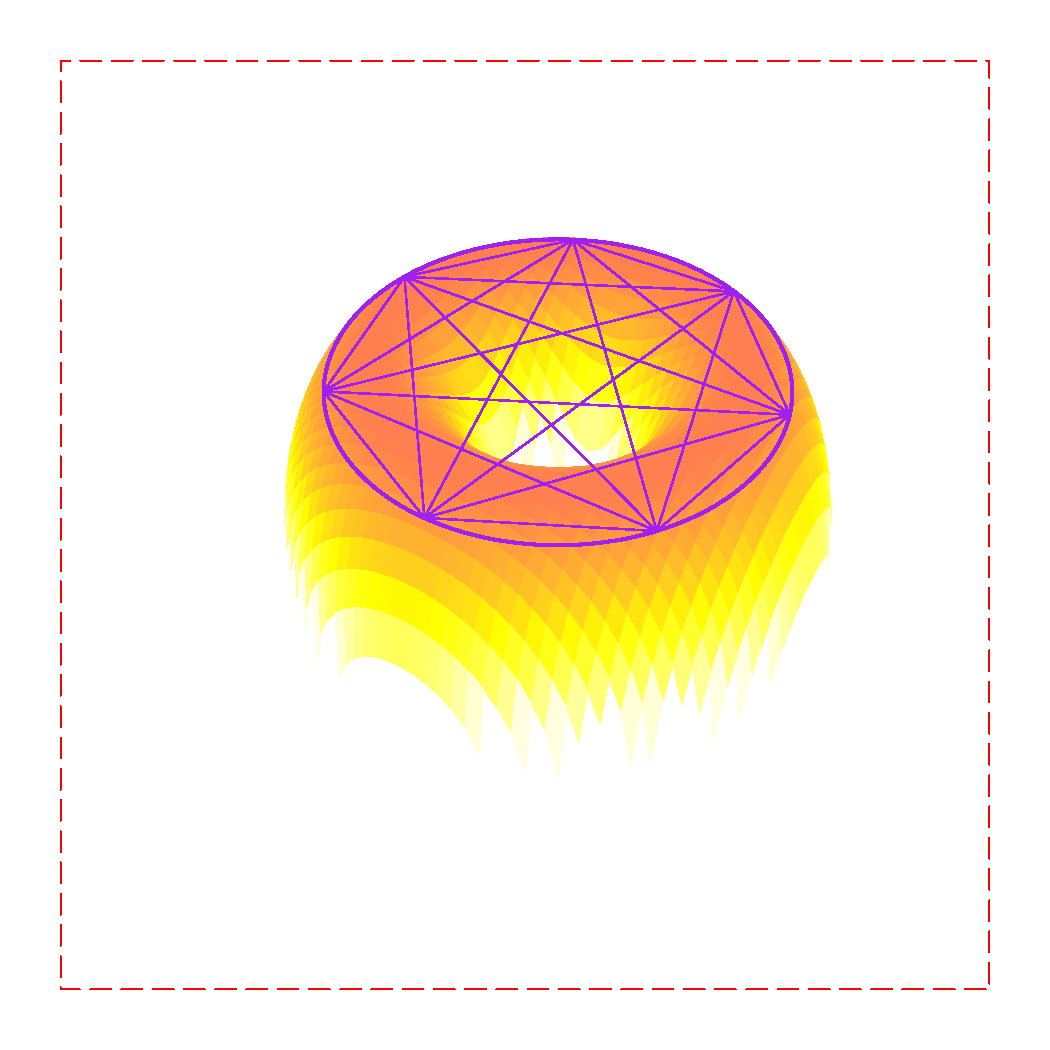
\includegraphics[height = 7cm, width = 7cm]{figure/gridGraphics_persp_demo_viewport2_1.pdf}
		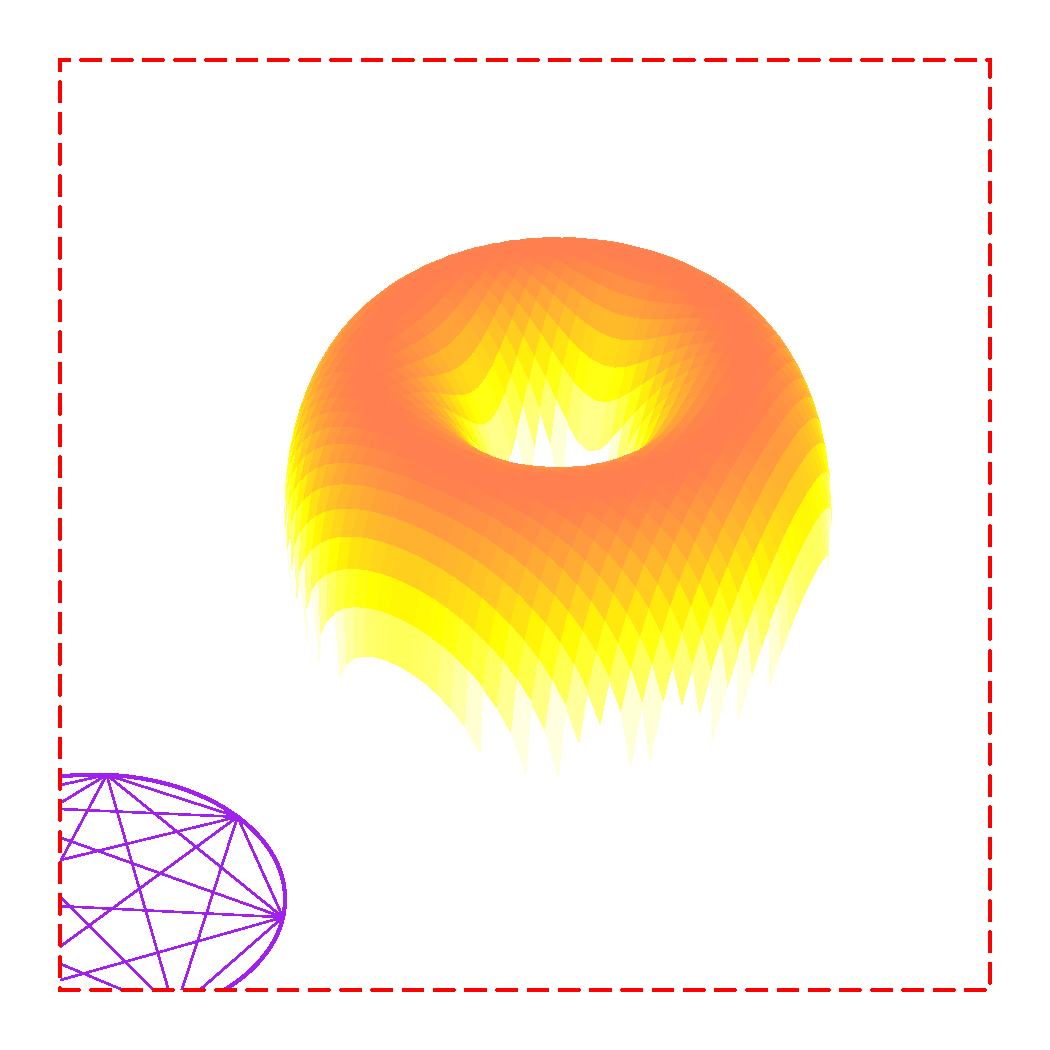
\includegraphics[height = 7cm, width = 7cm]{figure/gridGraphics_persp_demo_viewport2_2.pdf}
		\caption{A Rosette shape ring added to the tour(left-plot) on \textbf{graphics}, the right-plot reproduced the left-plot by \texttt{grid,echo()}. Although the tour is identical; the Rosette shape ring is on the incorrect location.}
		\label{figure_4.4}
	\end{center}
\end{figure}

The final problem will be to decide whether allows the concepts are drawn outside the plot region or not . Figure \ref{figure_4.5} shows the previous tour surface draw over the limit of the box. The left-plot is drawn by \textbf{graphics} which is the behaviors that we need to reproduce on \textbf{grid}. In \texttt{persp()}, there are three concepts are been drawn, the surface of perspective plot, the box that contains the surface and the axes plus the labels of axes. By default, \textbf{graphics} draw the surface by setting \texttt{clipping = "on"}. On the other hand, the surface will not exceed the limit of the plot region. However, the box and the axes may be drawn outside the plot region if it is necessary. Alternatively, the right plot is drawn by \textbf{grid} which indicates completely result comparing with the left plot (the surface is drawn over the plot region but the axes is not drawn outside the plot region). Due to the purpose of this paper, it is necessary to make sure the plots as identical as possible.\\
In \textbf{grid}, it is possible to define a viewport that either 'cut' the concepts if they are excess the limit of the viewport, or continuous draw them outside the viewport by setting the \texttt{clip} equal to be \texttt{"on"} or \texttt{"off"}.\\
The solution will be distinguished the clipping region for the concepts. Alternatively, the surface cannot excess the limit of the plot region therefore we need to "cut" the surface if it excesses the limit. On the other hand, we drawn the surface in the \texttt{clip = "on"}'s viewport. The box and the axes (include the labels and the units) are drawn in the \texttt{clip = "off"}'s viewport.\\
Since \textbf{gridGraphics} package already set up the clipping region, therefore it can be solved by navigating to the specific viewport and draw the concept of \texttt{persp()}. The following code is the action for solving this problem.

\newpage
\begin{lstlisting}[language = R]
## go to the viewport weather clip = 'off'
depth = gotovp(TRUE)
## draw the axes
PerspAxes(...)
upViewport(depth)

## go to the viewport weather clip = 'off'
depth = gotovp(TRUE)
## draw the Box
EdgeDone = PerspBox(0, xr, yr, zr, EdgeDone, trans, 1, lwd)
upViewport(depth)

## go to the viewport weather clip = 'on'
depth = gotovp(FALSE)
## draw the surface
DrawFacets(...)
upViewport(depth)
\end{lstlisting}\\

\begin{figure}[h]
	\begin{center}
		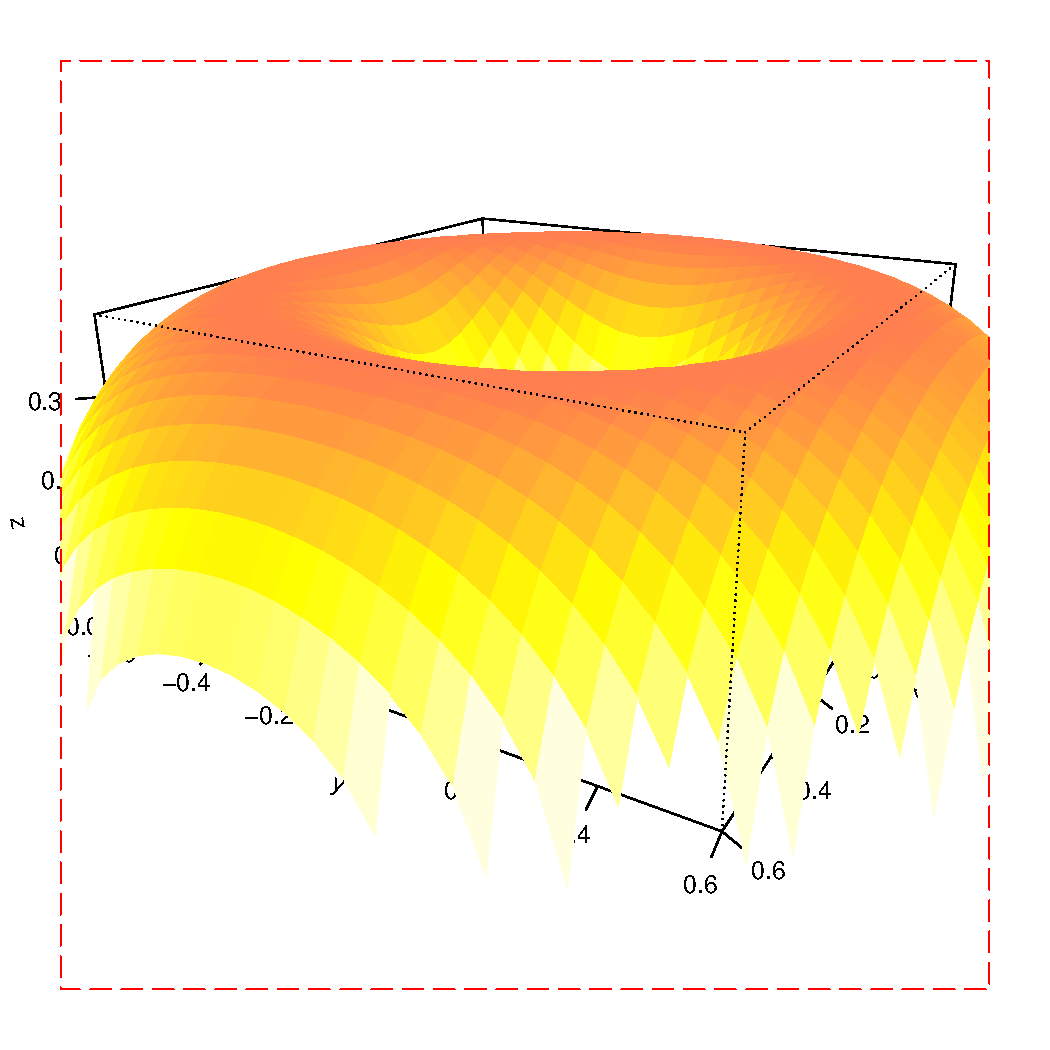
\includegraphics[height = 7cm, width = 7cm]{figure/gridGraphics_persp_demo_viewport3_1.pdf}
		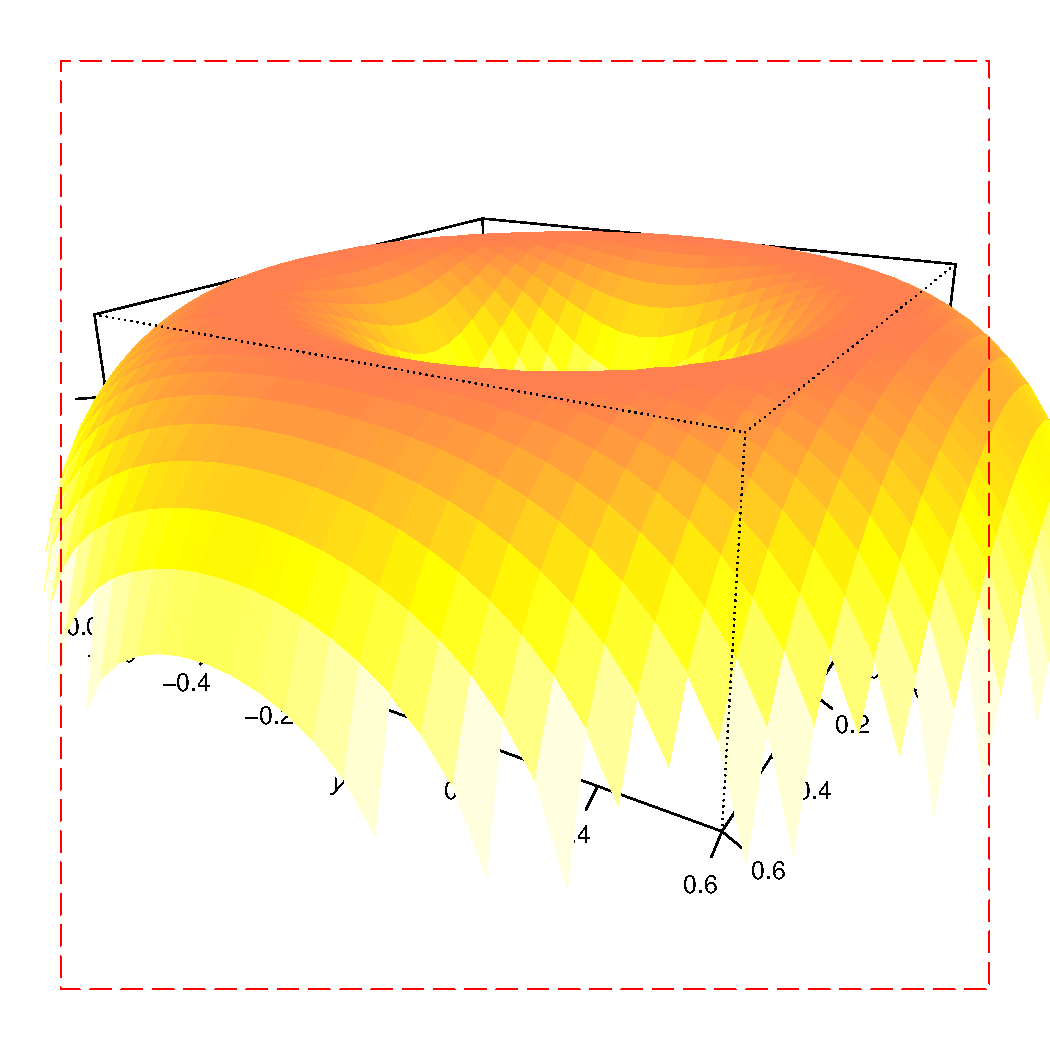
\includegraphics[height = 7cm, width = 7cm]{figure/gridGraphics_persp_demo_viewport3_2.pdf}
		\caption{A \textbf{graphics} \texttt{persp()} is drawn at the left. The red regions are the plot region for \textbf{graphics}(left plot) and the viewport region for \textbf{grid}(right plot). Clearly, the right plot is tried to reproduce the left plot, but the surface is not allowed excess the limit of the viewport, but the axes label and units are needs to be drawn even excess the limit.}
		\label{figure_4.5}
	\end{center}
\end{figure}



\section{Integrate \texttt{filled.contour()}}
Unlike \texttt{persp()}, \texttt{filled.contour()} is "made up" by multiple plots in one plot region. \textbf{gridGraphics} package will take care about most of the simple plots (such as the levels bar on the right-hand side of the plot, the titles, and the axes). (See Figure \ref{figure_1.3} or figure \ref{figure_3.6}).\\

\textbf{gridGraphics} fully convert the layout of \texttt{filled.contour()} to the viewport structure of \textbf{grid}, therefore we do not need to build or modify the viewport structure. However, it is necessary to "move" the filled contours into the correct location with the correct scale. On the other hand, we need to draw the filled contours in the correct viewport, provided by \textbf{gridGraphics}.\\

In Section 3.2, we discussed how a Filled Contour Plot been drawn by the \texttt{filled.contour()}. However, we only figure out who we drawn the main filled contour, but we still do not know how we display it. The next task is to display Filled Contour Plot in the correct location. Figure \ref{figure_4.6} shows the top-left is the contents of \texttt{filled.contour()}, which redrawn by using \textbf{grid} package. The red dotted rectangle is the viewport region. The next step is fill the blank region (top-right plot) by the top-left plot. The solution is similar to the first step of integrating \texttt{persp()}, that is, navigating to the correct viewport region and then drawn the filled contour. The following code is the solution in action.
\begin{lstlisting}[language = R]
## navigating to the correct viewport
depth = gotovp(TRUE)
## actual drawing
grid.polygon(...)
## reset
upViewport(depth)
\end{lstlisting}


\begin{figure}[h]
	\begin{center}
		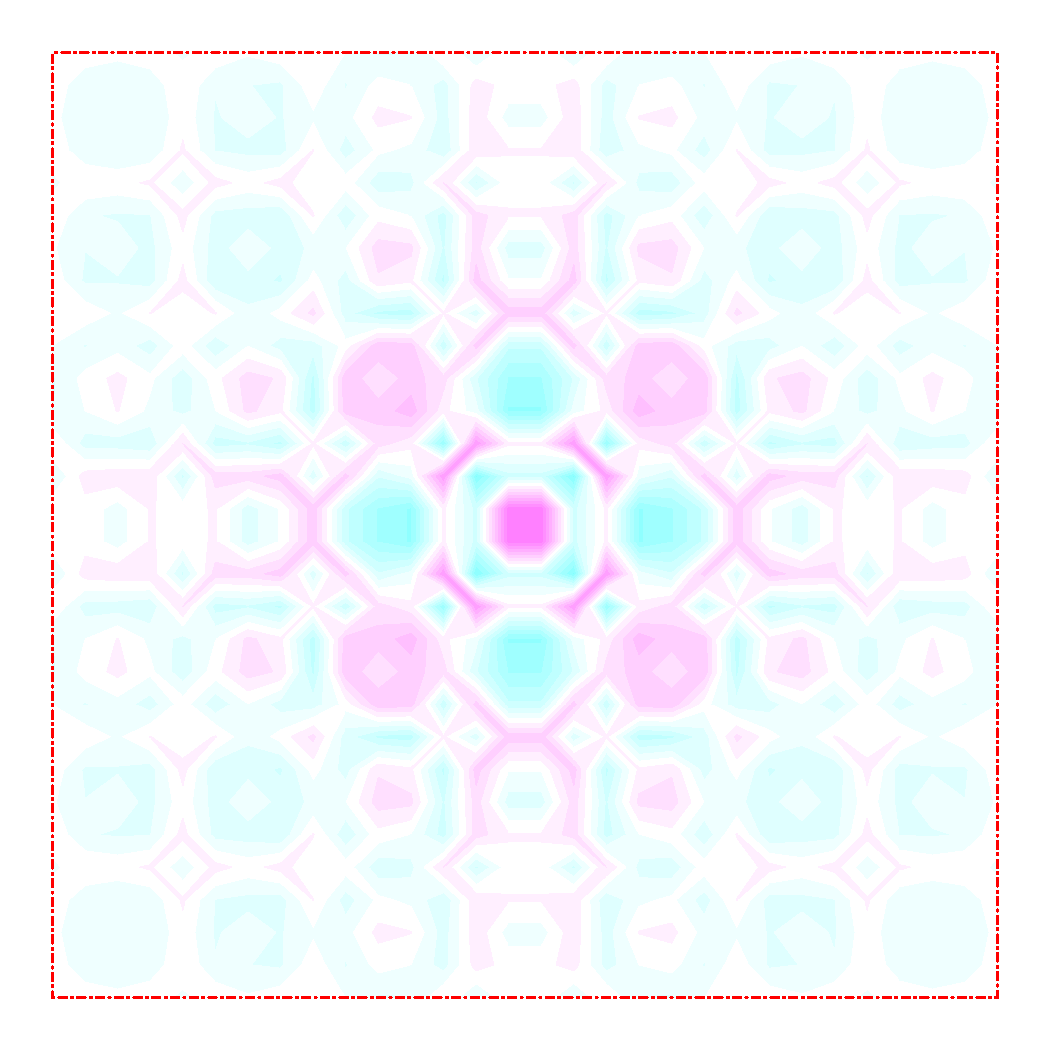
\includegraphics[height = 5cm, width = 5cm]{figure/filledContour_origin_02.pdf}
		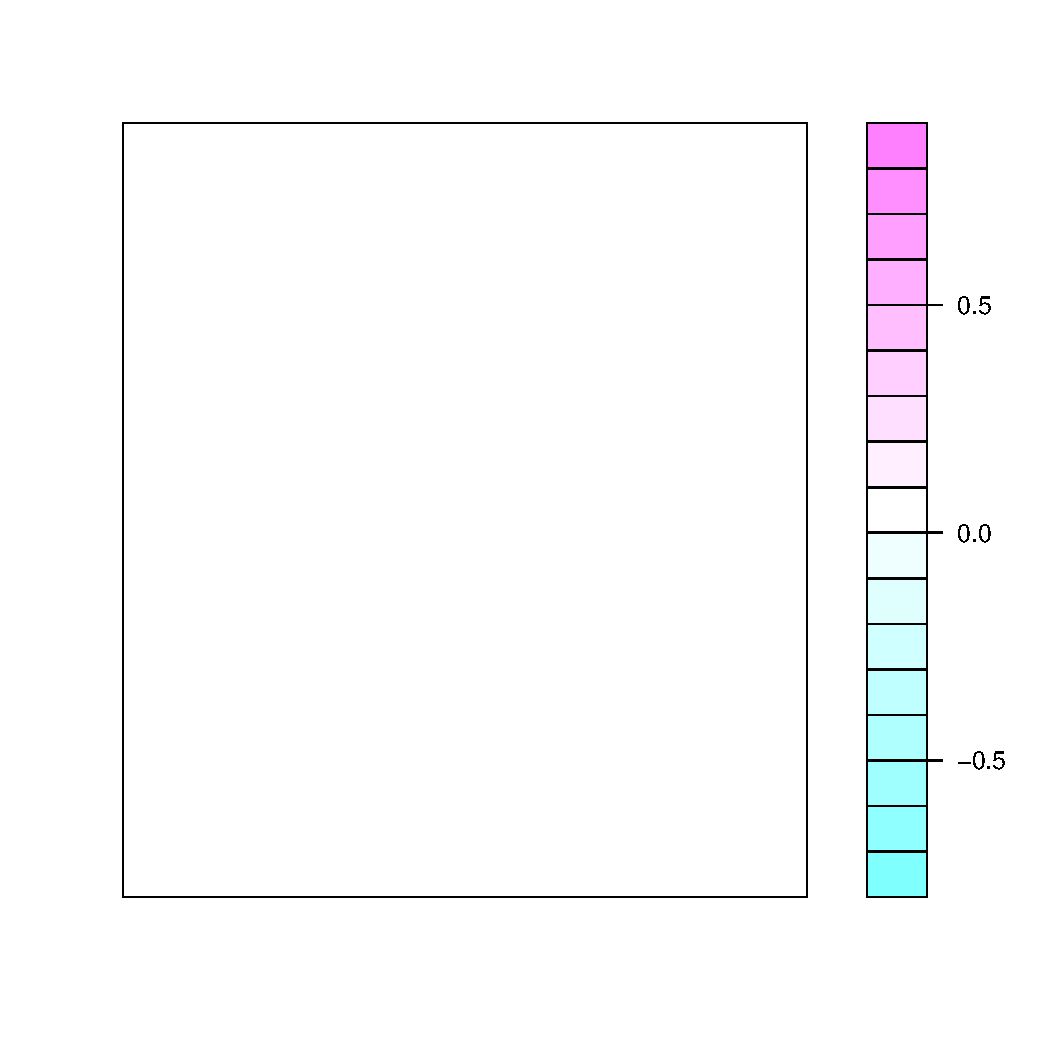
\includegraphics[height = 5.3cm, width = 6cm]{figure/filledContour_origin_03.pdf}
		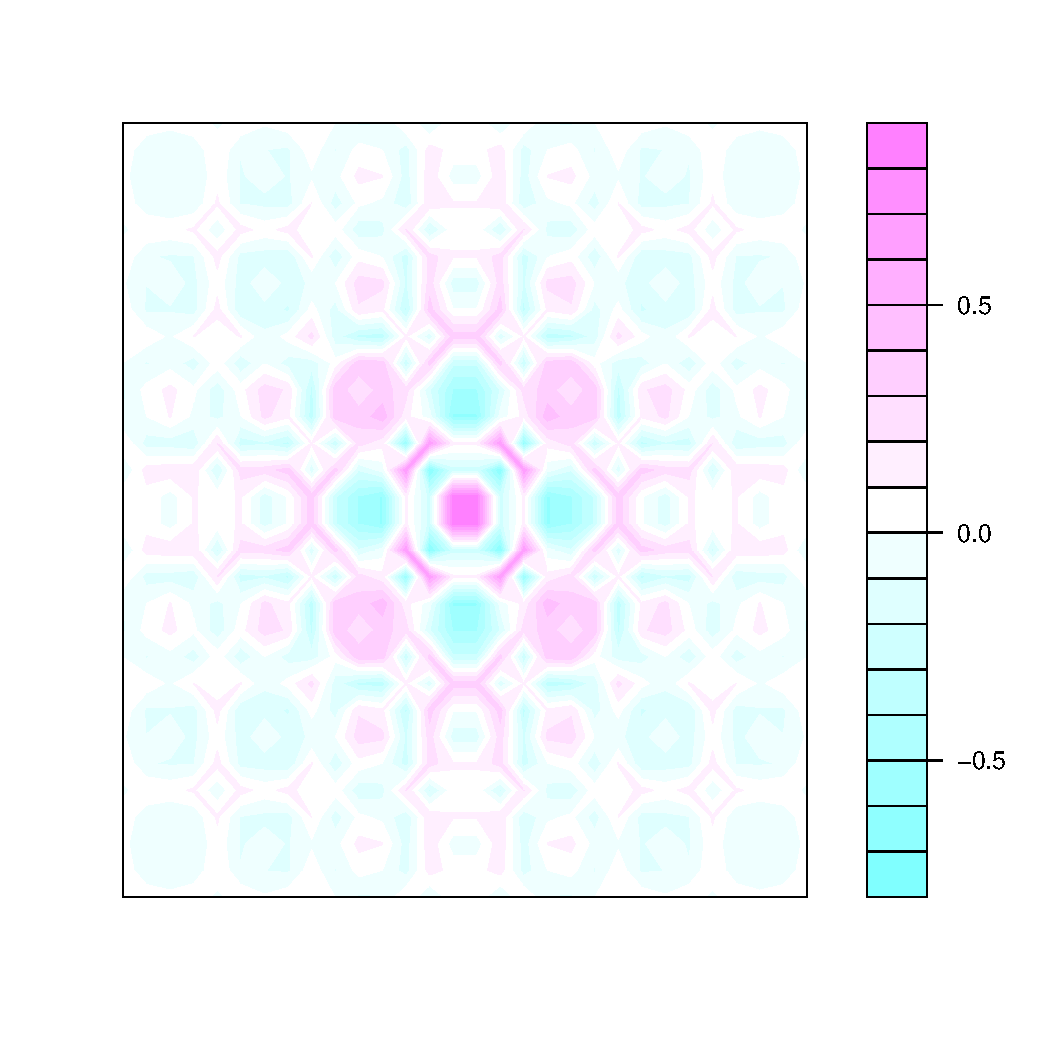
\includegraphics[height = 5.3cm, width = 6cm]{figure/filledContour_origin_01.pdf}
		
		\caption{The top-left filled contour are plotted by \textbf{grid}, top-right plot is the failed reproduce the \texttt{filled.contour()} by \texttt{grid.echo()} at the original state, and the bottom-center plot is the success reproduce the \texttt{filled.contour()} by \texttt{grid.echo()} after integrated to the \textbf{gridGraphics} package.}
		\label{figure_4.6}
	\end{center}
\end{figure}


\chapter{Testing}
The aim of this paper is to redraw Perspective Plots and Level (Contour) Plots using the \textbf{grid} package with an identical result to the \textbf{graphics} package. Every plot drawn by \textbf{grid} graphics should be not only identical to \textbf{graphics} by human eye, but also the machine 'thinks' they are identical. However, there are some tiny differences which cannot distinguish by human eye, for example, the color are differences at one pixel between two plots, or the colors of few area have one unit difference on red Channel distortion compare to the other plot. Therefore, we need software to detect those tiny differences.\\

\textbf{ImageMagick} \citep{ImageMagick} is the software that can be used for the comparison in this paper, it can create, edit, compose, or convert bitmap images and read and write images in a variety of formats (over 200). The features used in this paper is \texttt{compare}, which is a program to mathematically and visually annotate the difference between an image and its reconstruction.\\

The following example (See Figure \ref{chapter5.1}) are drawn two rotated sinc function, where the colors of the surface are close to each other and cannot be distinguish by human eyes. However, there is a difference for the colors, the plot in top-left ($rgb = 211, 182, 255$) has one color pixel higher on red channel than the plot in top-right ($rgb = 210, 182, 255$). The plot in bottom shows the difference, the region filled by red color is the difference, which is true because the color of the surface is different, the box and labels which have lighter color because they are mathematically and visually identical to each other. \\

\begin{figure}[h!]
	\begin{center}
		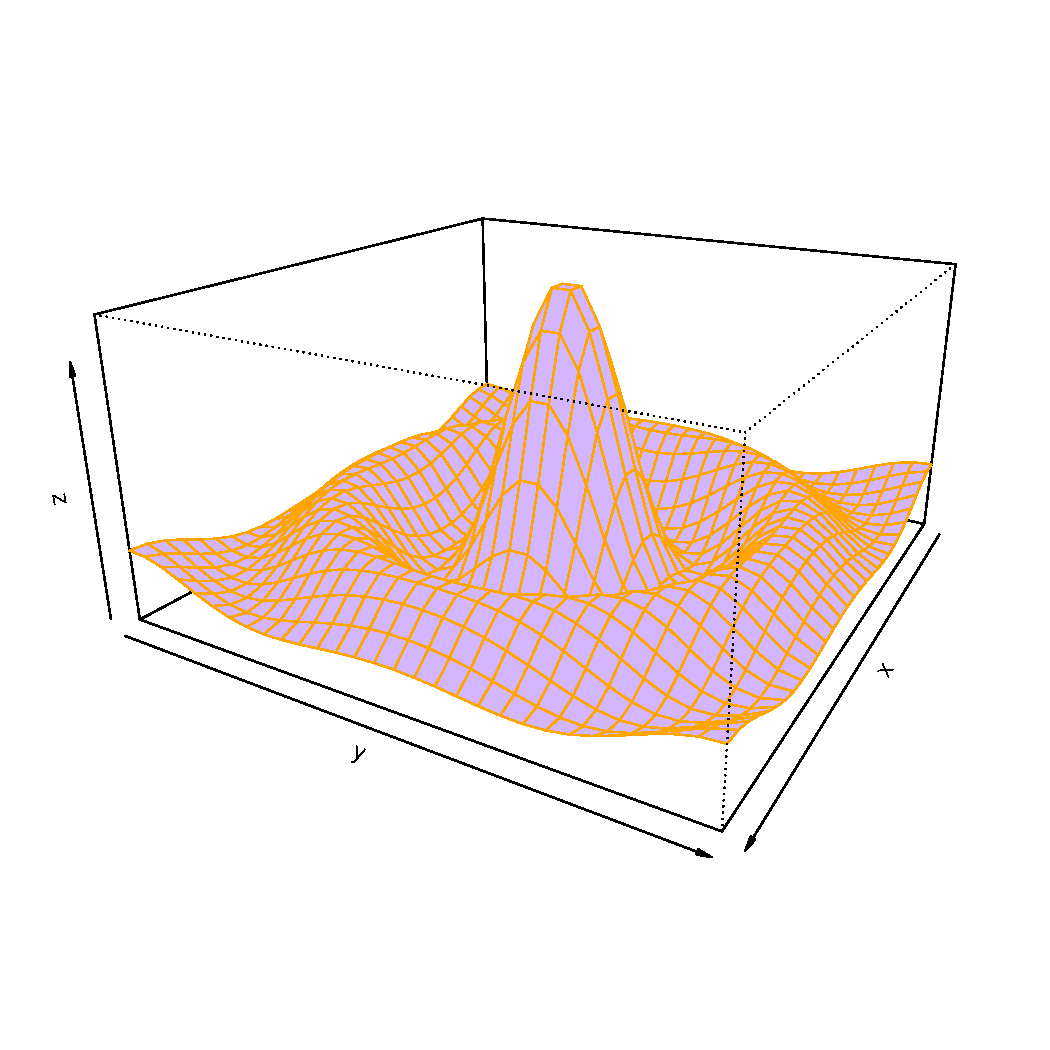
\includegraphics[height = 7cm, width = 7cm]{figure/Chapter5_example_01.pdf}
		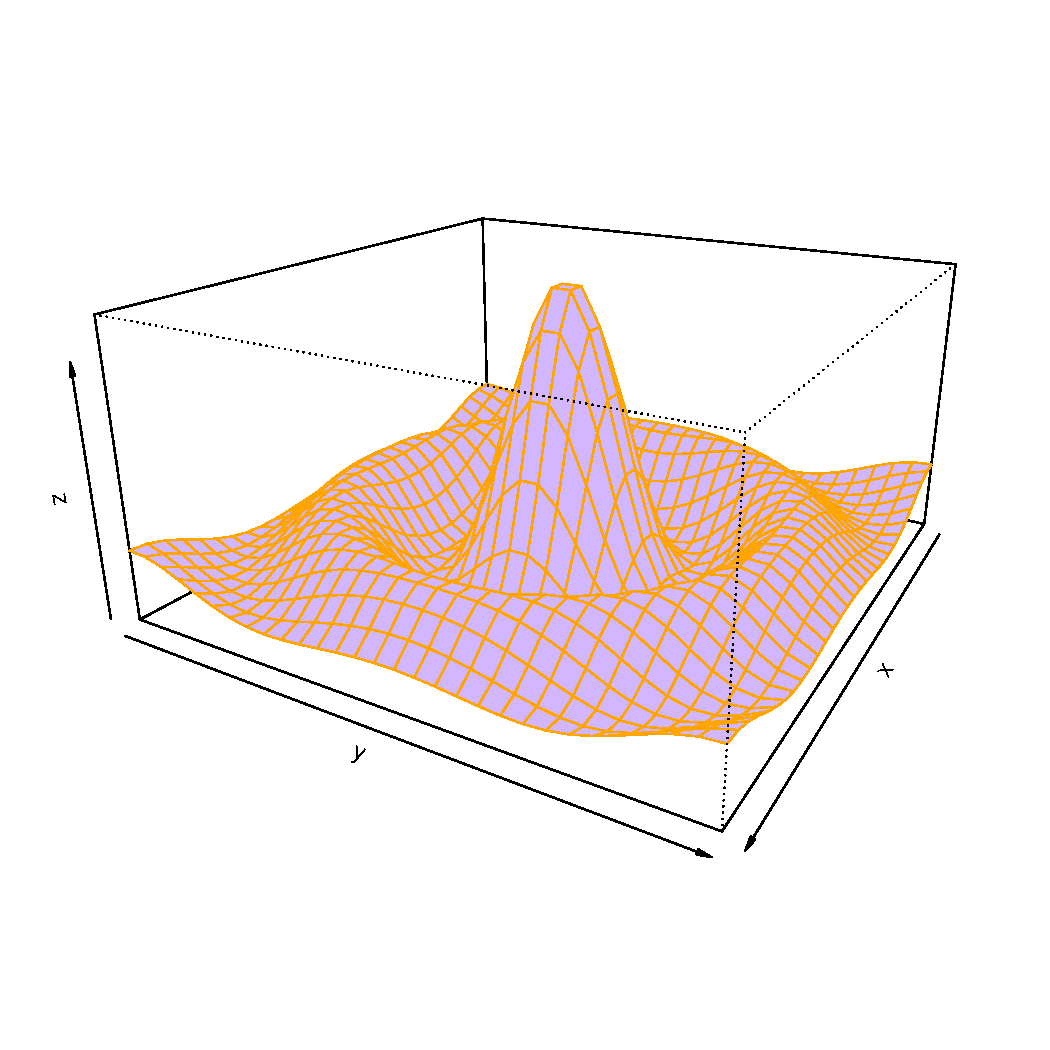
\includegraphics[height = 7cm, width = 7cm]{figure/Chapter5_example_02.pdf}
		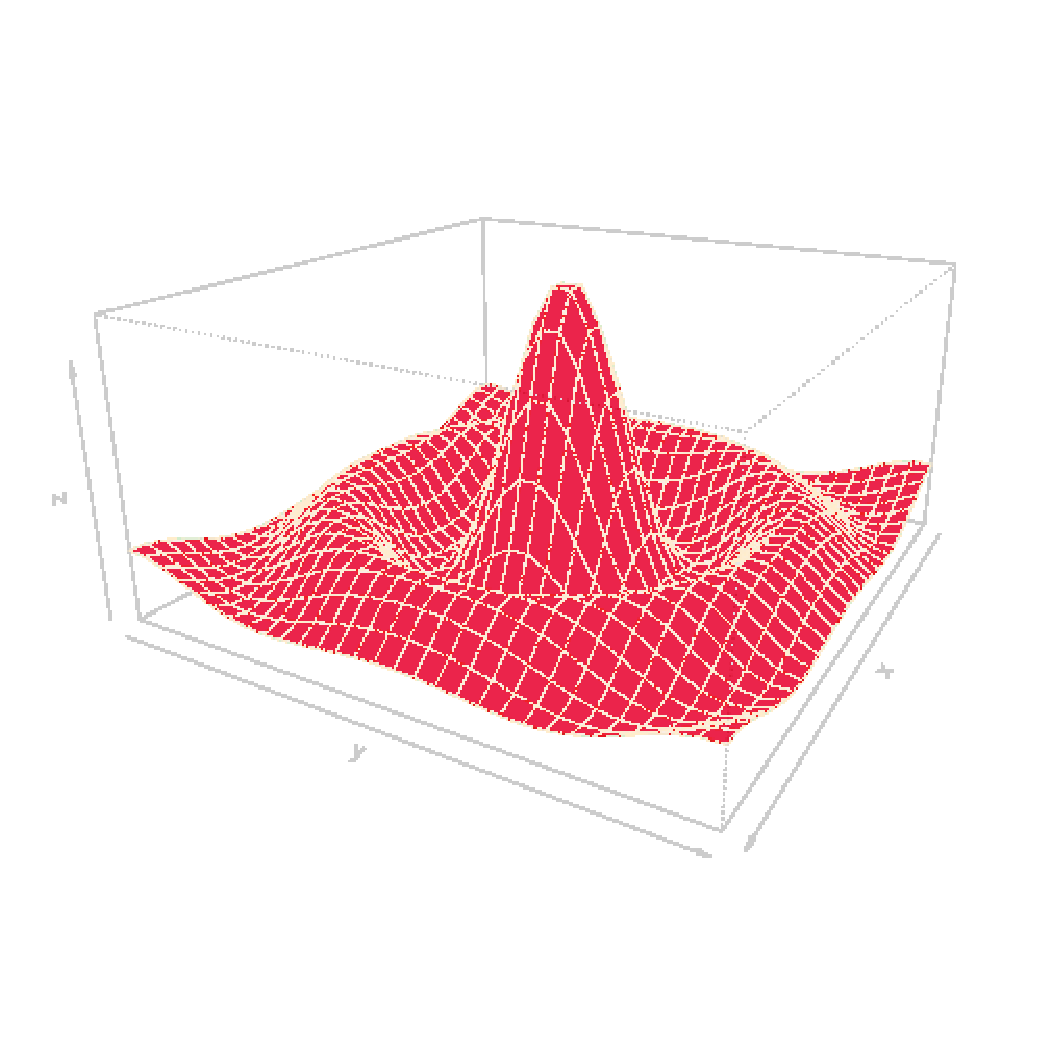
\includegraphics[height = 7cm, width = 7cm]{figure/Chapter5_example_03.pdf}
		\caption{The left plot looks identical to the plot at middle by human eyes, however, there is a tiny difference at the color of the surface, which been detected by the software, the red color indicated the difference.}
		\label{chapter5.1}
	\end{center}
\end{figure}

\newpage
To test whether a \texttt{persp()} plot and \texttt{filled.contour()} plot produce indentical results by \texttt{grid.echo()}, the \textbf{gridGraphics} provides a \texttt{plotdiff()} function. It will creates PDF and PNG files of a \textbf{graphics}-plot then compare with the result from \texttt{grid.echo()}. A PNG file will be created if there is any mathematically and visually difference. The \texttt{plotdiffResult()} will also provide to summarize the multiple results called by \texttt{plotdiff()}.\\
  The Figure \ref{chapter5.2} and Figure \ref{chapter5.3} shows all the \texttt{persp()} plot and \texttt{filled.contour()} plot drawn by \textbf{graphics}-based are mathematically and visually identical when they converted to \textbf{grid}, by using the \texttt{grid.echo()}.


\begin{figure}[h]
	\begin{center}
		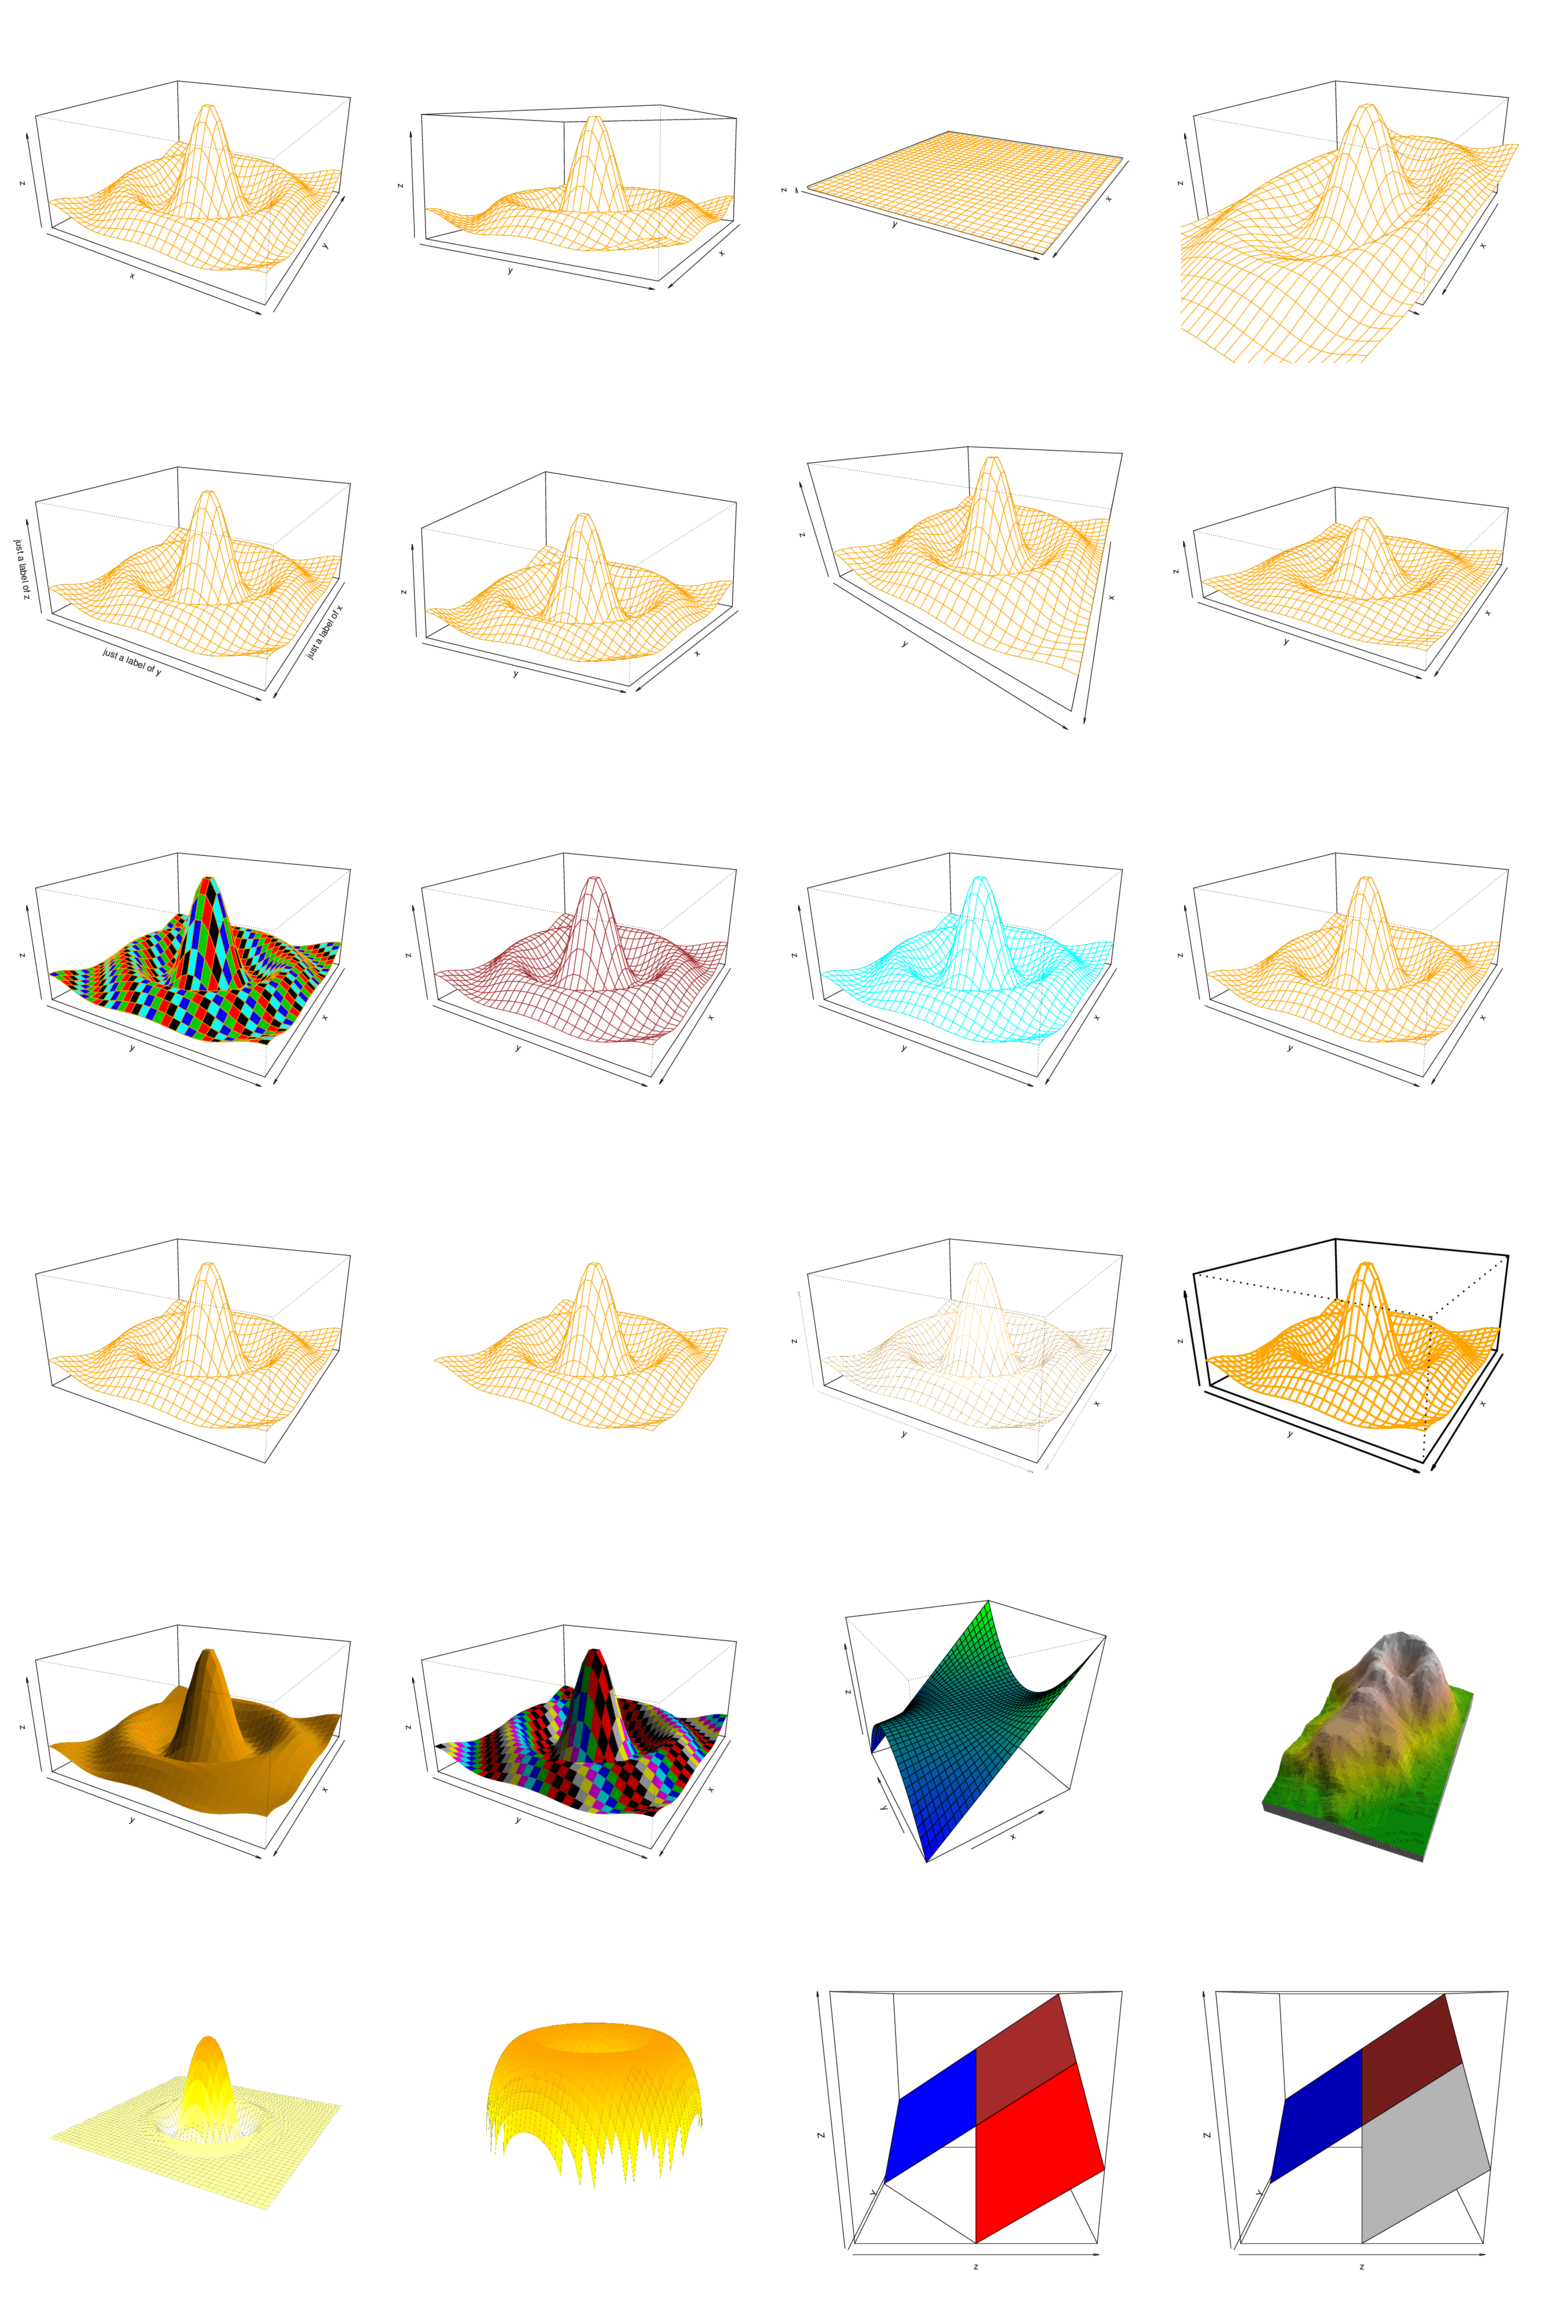
\includegraphics[height = 24cm, width = 16cm]{figure/montage/persp-montage.png}
		\caption{A set of perspective plots, which passed the identical test by ImageMagick}
		\label{chapter5.2}
	\end{center}
\end{figure}


\begin{figure}[h]
	\begin{center}
		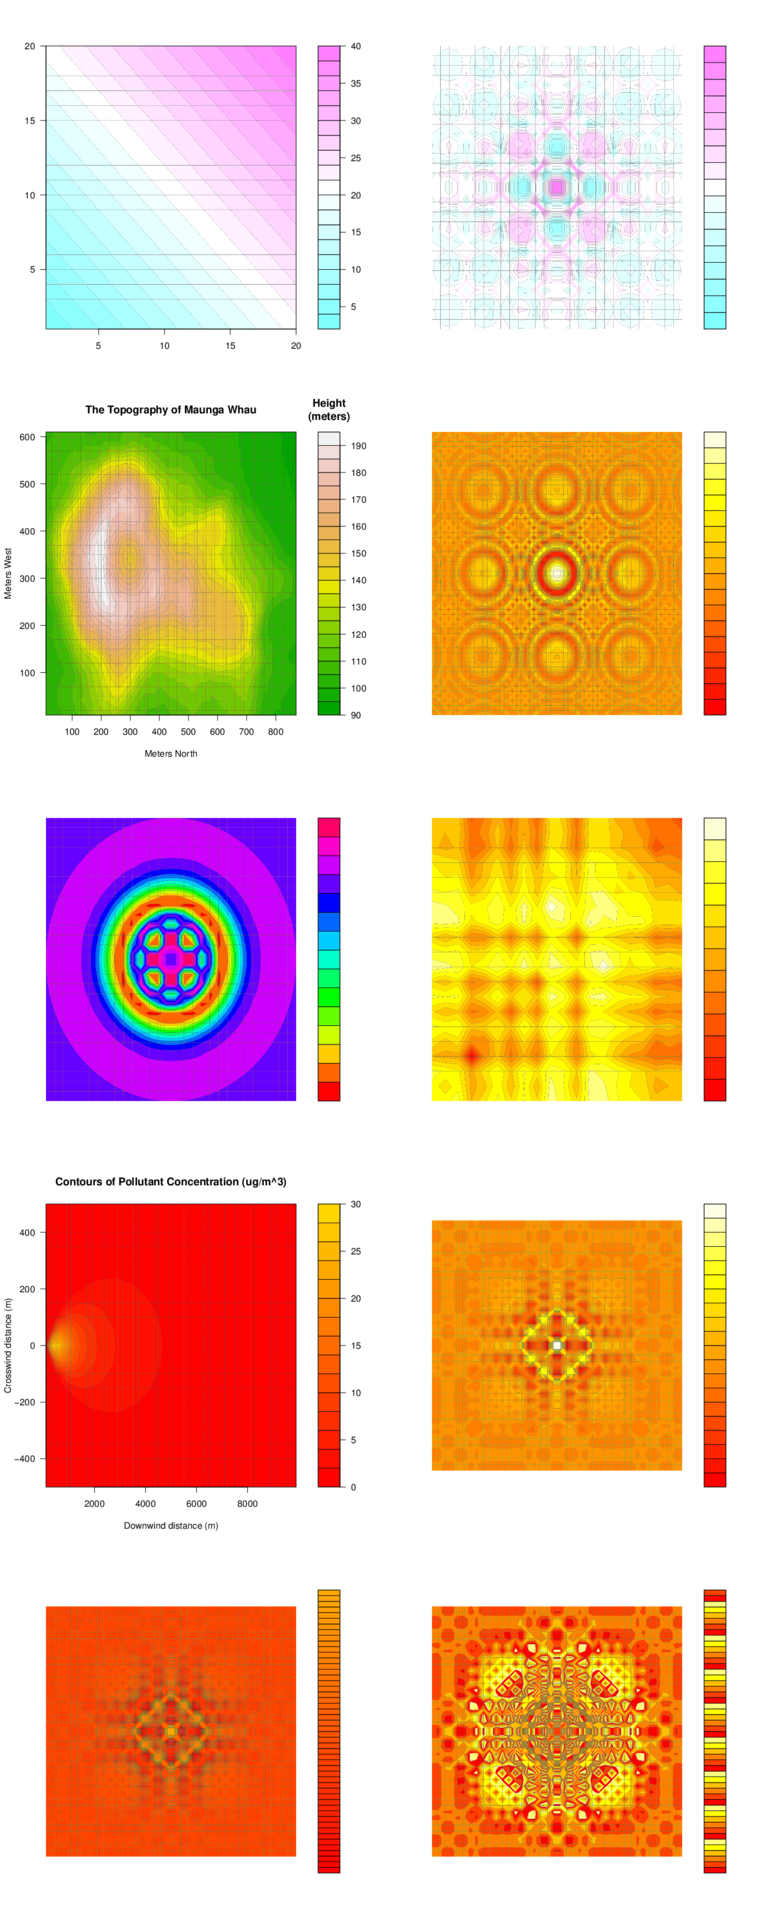
\includegraphics[height = 24cm, width = 12cm]{figure/montage/filled-contour-montage.png}
		\caption{A set of filled contour plots, which passed the identical test by ImageMagick}
		\label{chapter5.3}
	\end{center}
\end{figure}


\chapter{Example}
The \texttt{persp()} plot and \texttt{filled.contour()} plot are now supported by \textbf{gridGraphics}. This means most of the plots that drawn by \texttt{persp()} and \texttt{filled.contour()} by \textbf{graphics} package now is able to reproduce by \texttt{grid.echo()} on \textbf{grid}. The advantage of \textbf{grid} is \textbf{grid} is more flexible than \textbf{graphics}. For example, a plot drawn by \textbf{grid} can record the viewport structure and we may draw and edit any plot features within different viewport easily.


\section{Example to solution}
The \texttt{persp()} and \texttt{filled.contour()} are now can been edited more easily since they are integrated to \textbf{gridGraphics}. Another Torus shape is drawn by \textbf{graphics} (See Figure \ref{Example_6.3}), it has been redrawn on \textbf{grid} by \texttt{grid.echo()} and then we can listing the grobs of this plot. Since we are only drawing the surface, and the surface is formed by polygons. Then we can modify the features of the polygons easily by using \texttt{grid.edit}. In this example, we changed the white color (with opacity is 0) to purple (with opacity is 0.3).\\
\begin{Schunk}
\begin{Sinput}
> Torus_shape(col = 'NA', border = 'gray', box = FALSE)
> grid.echo()
> grid.ls()
\end{Sinput}
\begin{Soutput}
GRID.polygon.4
\end{Soutput}
\begin{Sinput}
> newCol = rgb(160/255, 32/255, 240/255, alpha = 0.3)
> grid.edit(grid.ls(print = FALSE)$name[1], gp = gpar(fill = newCol))
\end{Sinput}
\end{Schunk}

\begin{figure}[h]
	\begin{center}
		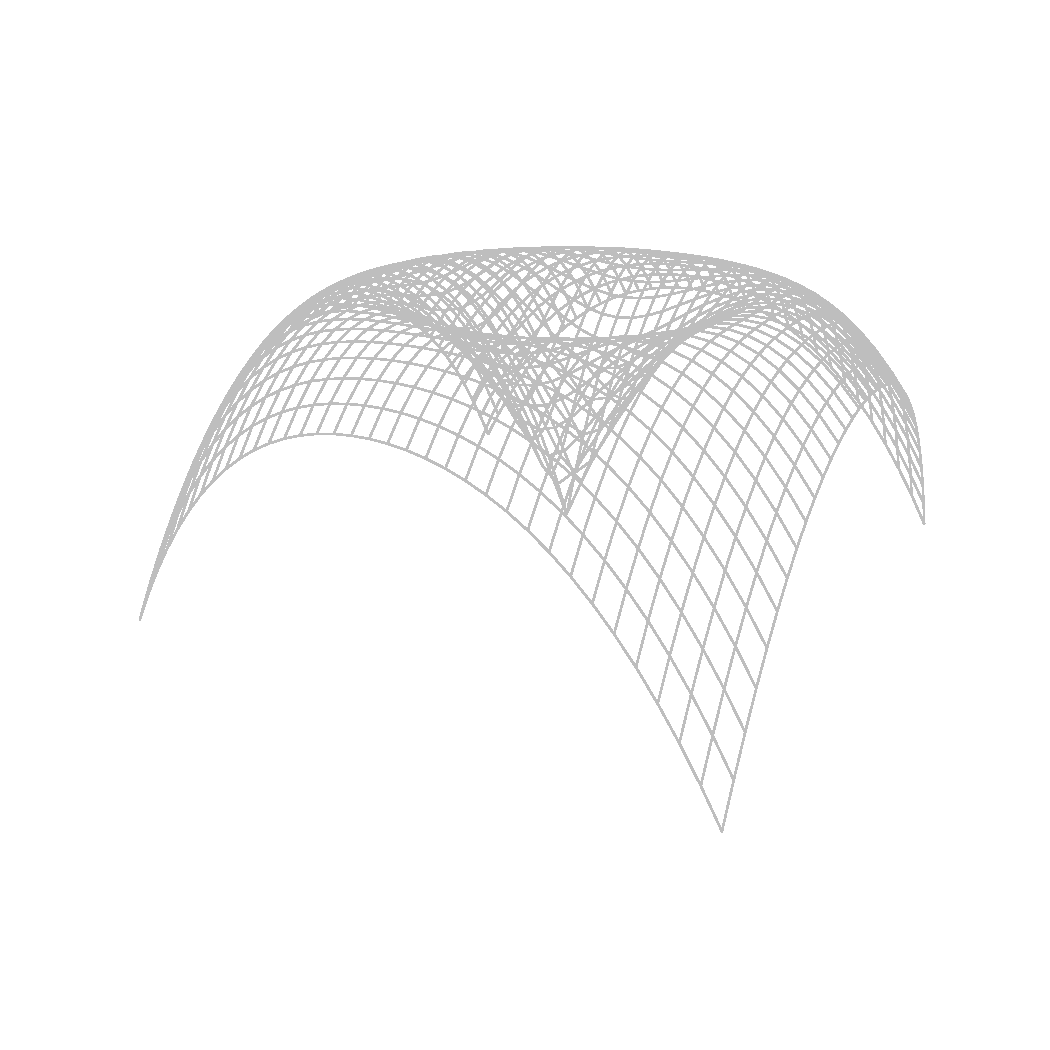
\includegraphics[height = 7cm, width = 7cm]{figure/Chapter6_example_1_2.pdf}
		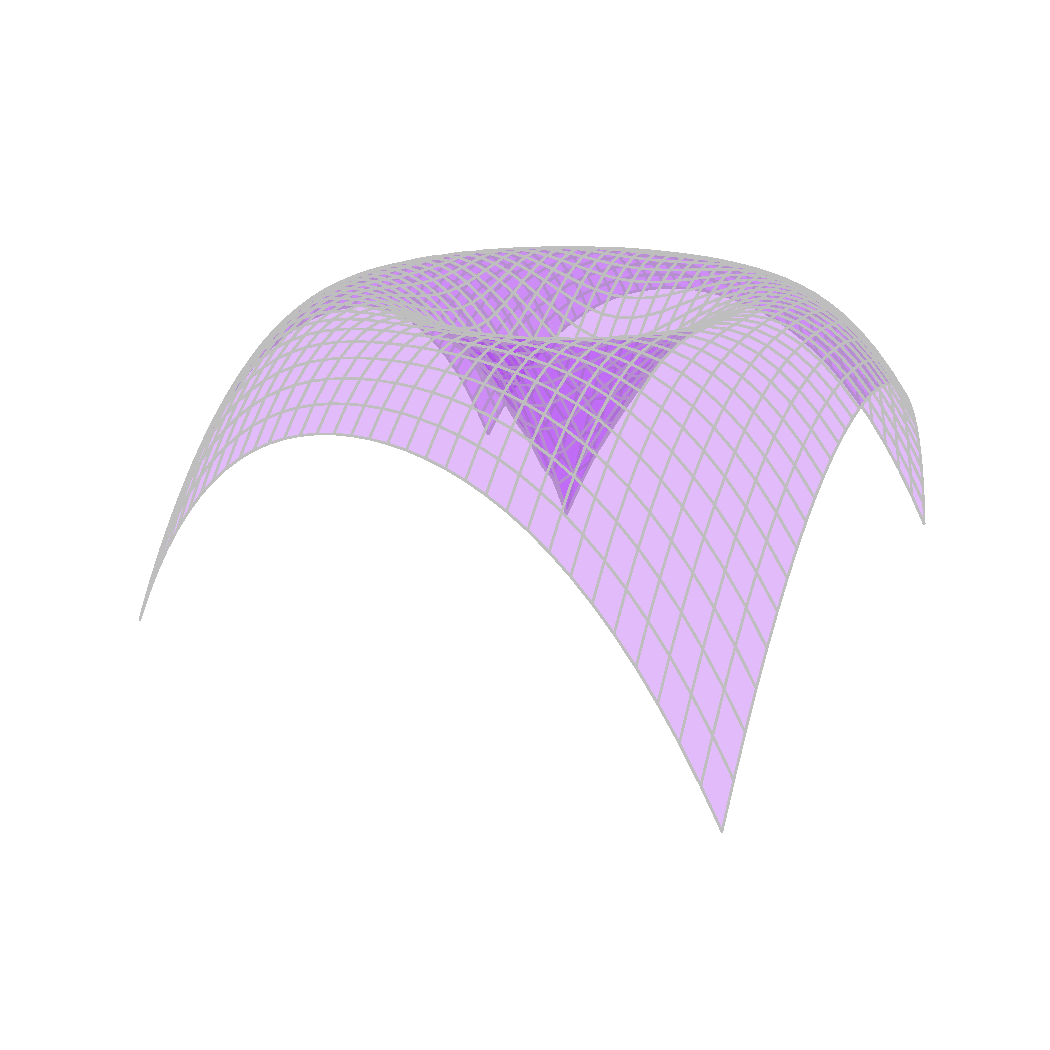
\includegraphics[height = 7cm, width = 8cm]{figure/Chapter6_example_1_3.pdf}
		\caption{The left \texttt{persp()} plot is drawn by \textbf{graphics}, where the right plot is been drawn by redrawn the left plot on grid (\texttt{grid.echo()}) and then modify the colors by \texttt{grid.edit()}}
		\label{Example_6.3}
	\end{center}
\end{figure}


\newpage
Another benefit that \textbf{grid} graphics provides is that we can get a grid graphical object. For example it is possible to get the colors of the filled contour plot which drawn by \textbf{grid} (see following codes and figure \ref{Example_6.1} ) and then transform these colors to the corresponding colors with Chroma removed in Hue Chroma Luminance (HCL) space.
\begin{Schunk}
\begin{Sinput}
> fill.contour.plot()
> grid.echo()
> ## get the colors of filled.contour() drawn by grid
> poly.obj = grid.get(grid.ls(print = FALSE)$name[3])
> rect.obj = grid.get(grid.ls(print = FALSE)$name[1])
> ## display the first 6 colors
> head(poly.obj$gp$fill)
\end{Sinput}
\begin{Soutput}
[1] "#C6DE00FF" "#A7D700FF" "#C6DE00FF" "#A7D700FF" "#A7D700FF" "#C6DE00FF"
\end{Soutput}
\begin{Sinput}
> ## transform the colors
> colpoly = colorspace::desaturate(poly.obj$gp$fill)
> colrect = colorspace::desaturate(rect.obj$gp$fill)
> ## modify the colors
> grid.edit(grid.ls(print = FALSE)$name[3], gp = gpar(fill = colpoly))
> grid.edit(grid.ls(print = FALSE)$name[1], gp = gpar(fill = colrect))
\end{Sinput}
\end{Schunk}



\begin{figure}[h!]
	\begin{center}
		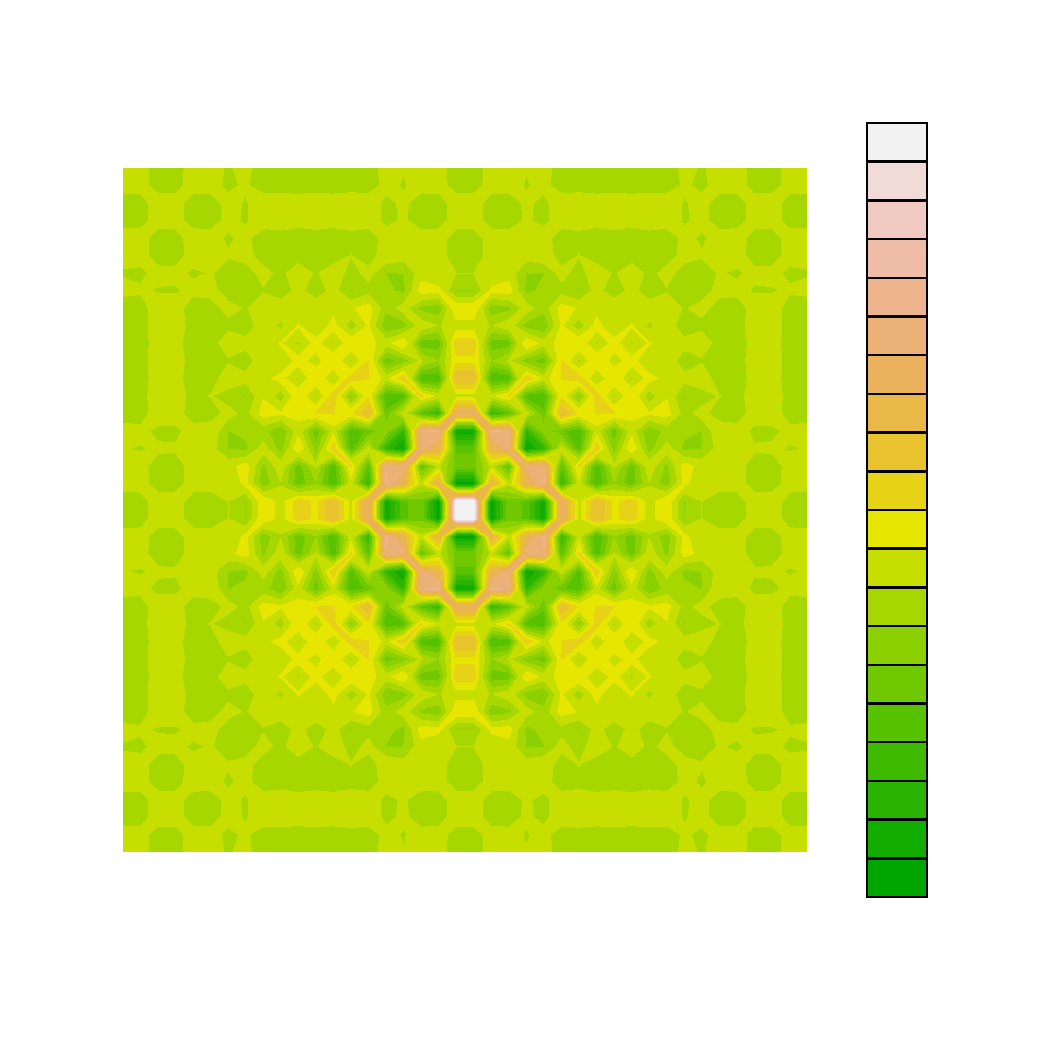
\includegraphics[height = 7cm, width = 7cm]{figure/Chapter6_example_2_2.pdf}
		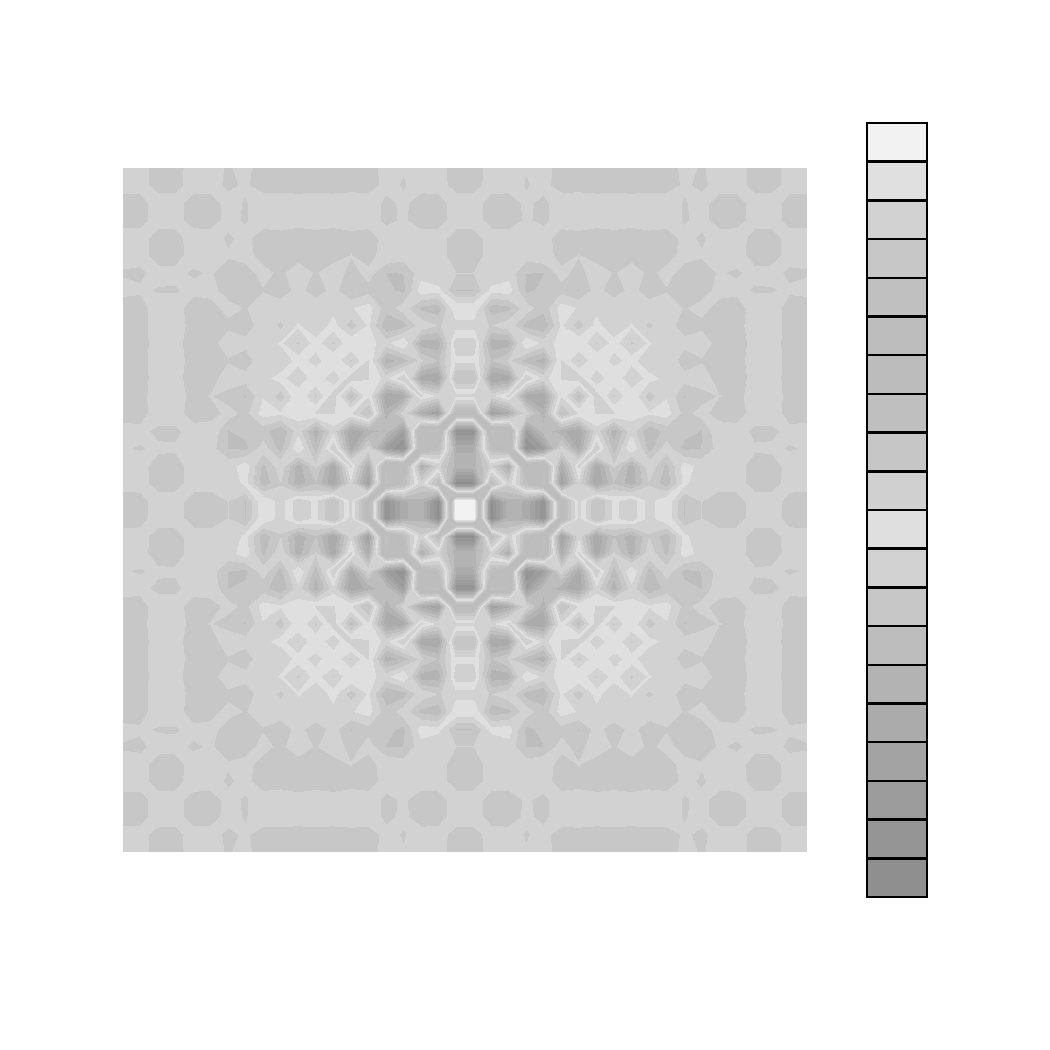
\includegraphics[height = 7cm, width = 7cm]{figure/Chapter6_example_2_4.pdf}
		\caption{The left filled contour plot is drawn by \textbf{graphics}, where the right plot is been drawn by redrawn the left plot on grid (\texttt{grid.echo()}) and then modify the colors by \texttt{grid.edit()}}
		\label{Example_6.1}
	\end{center}
\end{figure}

\newpage
\section{An advance example}
In the \textbf{graphics} package it is very normal to draw two or more plots in the plot region. However, it is not allowable to combine the \texttt{filled.contour()} with any other kind of plots together within one plot region, because \texttt{filled.contour()} will create the layout itself when it is called. Therefore, even if we specify a layout before plotting, the \texttt{filled.contour()} will overwrite the layout.\\

The viewport structures of \textbf{grid} provides more flexibility than the layout of \textbf{graphics}, which allows us draw any other plots with \texttt{filled.contour()} within one page. The idea is to create a viewport before drawing any plots (said Root viewport), then push a viewport within the Root viewport for drawing a grid version of \texttt{filled.contour()} so that the \texttt{filled.contour()} will only modify the structure of its own viewport but not overwrite the Root viewport.\\
\begin{figure}[H]
	\begin{center}
		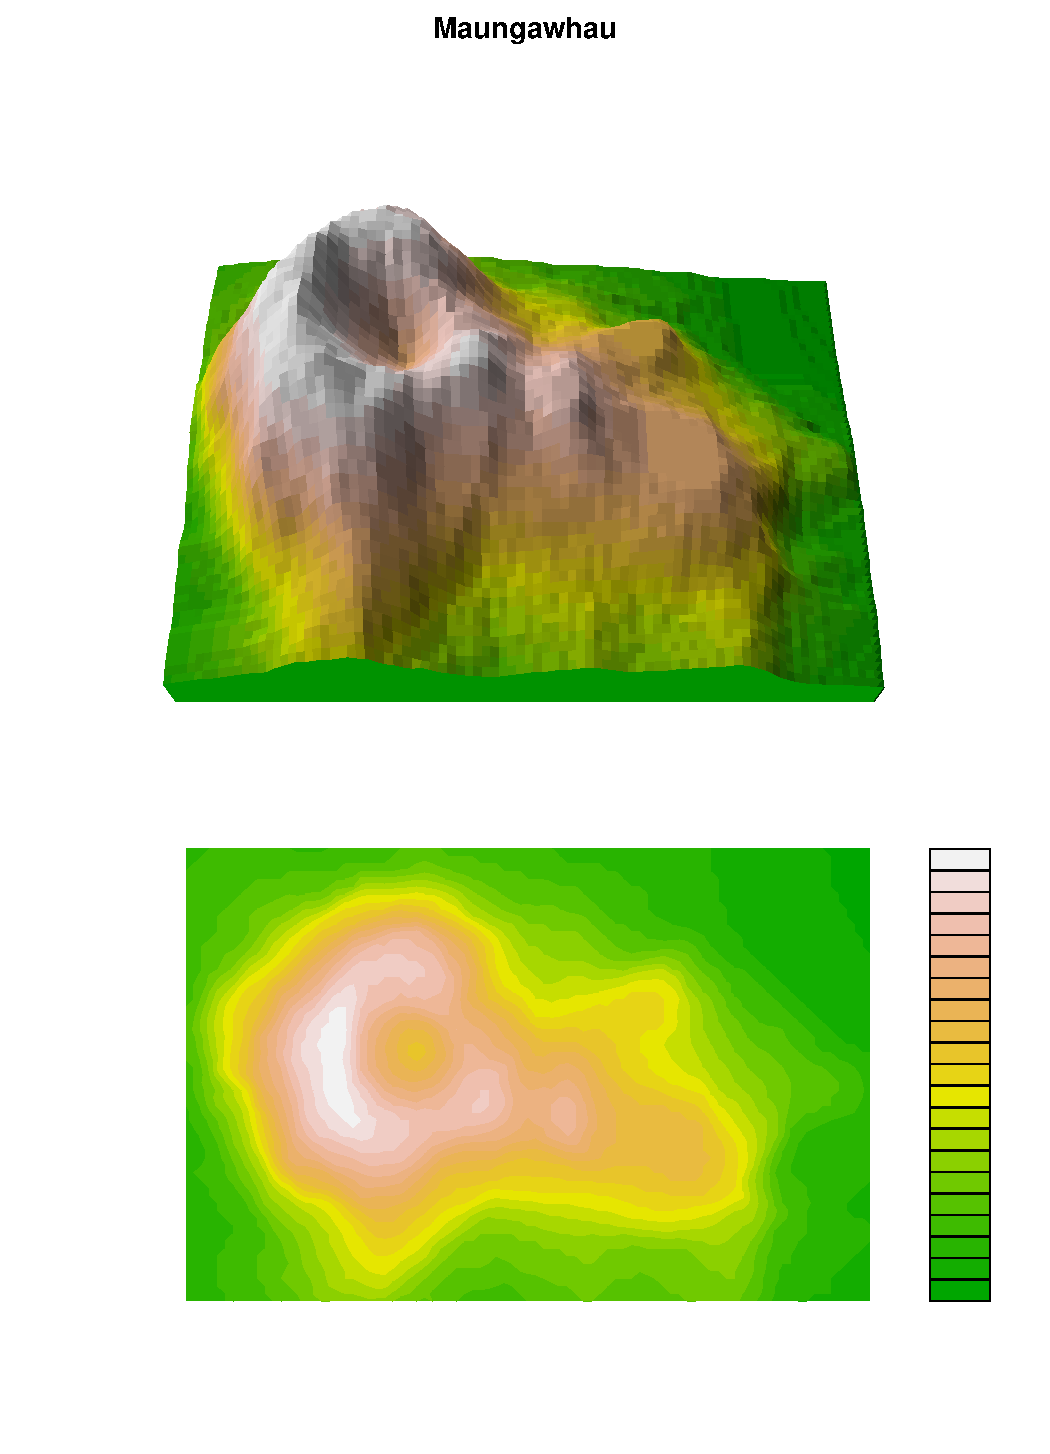
\includegraphics[height = 16cm, width = 12cm]{figure/Chapter6_example_3_1.pdf}
		\caption{The top plot shows the shape of Maunga whau volcano, where the bottom figure shows the level contour (i.e. the height)}
		\label{Example_6.2.1}
	\end{center}
\end{figure}


\newpage
\section{A more advance example}
\subsection{Basic concepts}
The benefit that \textbf{gridGraphics} is that the \textbf{graphics} plot converted to \textbf{grid} that contains the \textbf{grobs} and \texbf{viewport} with names. The \texttt{gridSVG} \citep{gridSVG} package can export this plot to SVG format image, which it contains the information of the \textbf{grobs} and \textbf{viewports} names. Therefore, the \textbf{JavaScript} \citep{javascript} can interact with the SVG image more easily because the SVG elements contain every graphical element of the image.\\

SVG (Scalable Vector Graphics) \citep{SVG} is a two-dimensional vector image format with XML-based. A SVG format graphics can support for interactivity and animation which most of the \texttt{R} graphics system is not supported or it is difficult to implement by \texttt{R} graphics system.\\

\begin{lstlisting}
<circle id = "circle1" 
    cx="50" cy="50" r="40" 
    stroke="black" stroke-width="3" 
    fill="red" />
\end{lstlisting}

The previous codes created the circle filled with red color (See Figure \ref{Example_6.3.0}), where the radius is 40 units. As we see, the color of the circle is defined on the \texttt{circle} element which is the \texttt{fill = "red"} in its attribute. To modify the color of the circle, the first step to find the \texttt{circle} element. The element contains an \texttt{id}, its value is \texttt{"circle1"}.\\

The following codes is coded with \texttt{JavaScript}. It interacts with the SVG image that changes the color of the circle from red to yellow, when a mouse moves into the circle region. The key step of this interactivity will be track the circle element and modify its color.\\

The method for tracking the \texttt{circle} element is to find the elements where its \texttt{id} attribute is \texttt{"circle1"}. Therefore, the \texttt{getElementById()} method is used. It will return the element that has the ID attribute with the specified value. After the circle element is tracked, we can simply add a \texttt{onmouseover} event to it. That is, the color of the circle will change only if a mouse moving into the circle. The \texttt{onmoveover} function is called when the event is activated.\\ 

\begin{lstlisting}
Onmove = function(){
    this.setAttribute('fill', "yellow");
}
var Oncircle;
Oncircle = document.getElementById("circle1");
Oncircle.onmouseover = Onmove;
\end{lstlisting}

\begin{figure}[h]
	\begin{center}
		
\includegraphics[height = 1.45cm, width = 1.6cm]{figure/svg/svgdemo0.PNG}
		\hspace{4cm}
		
\includegraphics[height = 1.5cm, width = 1.5cm]{figure/svg/svgdemo1.PNG}
		\caption{The left circle is created with svg imgae, the right circle is changed color to yellow then the mouse enter the region of the circle. }
		\label{Example_6.3.0}
	\end{center}
\end{figure}

\subsection{The sinc surface}
Since those actions cannot been achieved by R graphics system. The first step is to export the plot into
SVG image. To do that, the \texttt{gridSVG} package is required. The following codes are used for export the SVG image (See Figure \ref{Example_6.3.01}). surface() is the ''wrap'' function for drawing the sinc surface perspective plot.
addFeatures() is creating the texts and the little boxes of color at the top-left region in the plot.
It also creates some hidden objects which are all invisible unless the specific action is activated. A
JavaScript is imported for supporting the animations by using grid.script(). Finally we exported
the SVG image by \texttt{grid.export()}
\\

\begin{lstlisting}[language = R]
## draw a surface
surface()  
## add the button at the top-left of the plot and hidden objects prepare for animation
addFeatures() 
## import the javascript file into the SVG image
grid.script(file="example.js") 
## export the SVG image
grid.export("example.svg", strict = FALSE) 
\end{lstlisting}

\begin{figure}[h]
	\begin{center}
		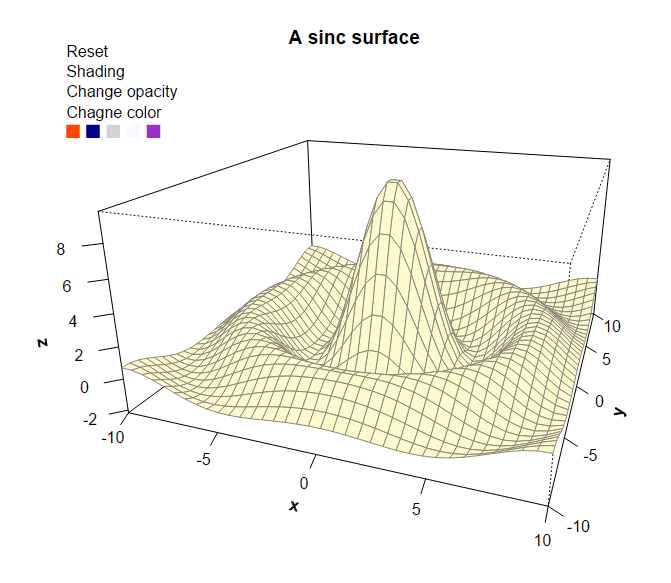
\includegraphics[height = 11cm, width = 12cm]{figure/svg/origin_1.PNG}
		\caption{A SVG image of the sinc surface perspective plot}
		\label{Example_6.3.01}
	\end{center}
\end{figure}




In this example, we are going through the animation of the following action. Since it is not possible to see the full animation. To see the full animation, please vist \href{https://github.com/yeamin1/MasterProject/blob/master/report/svg}{my github}

\begin{itemize}
	\item Changing the color of the surface
	\item Changing the opacity of the surface
	\item Shading the surface
	\item Highlighting the specific fragment of the surface and showing its z-value  
\end{itemize}
\\

\subsubsection*{Animation of Changing the color of the surface}
Similar to the circle example, we change the color of the surface by locating the elements that contain the surface then modify the color. However, the complicate part will be the animation creation. The animation of \texttt{JavaScript} can be done by programming gradual change in the attribute of the elements. The animation will look continuous when the time interval between every change are small.\\

The following code is key step for creating the animation (See Figure \ref{Example_6.3.1}). The \texttt{animate()} can produce all the action that we discussed previously. The \texttt{frame()} in the \texttt{animate()} will change the color of the surface gradually every time it been called. The \texttt{setInterval(frame, 30)} will call the \texttt{frame()} every 30 milliseconds. On the other hand, the color of the surface will be changed gradually every 30 milliseconds. This action will be activated when user clicks the red boxes.

\begin{lstlisting}[language = JavaScript]
animate = function(...){
    setInterval(frame, 30)
    function frame() {
      ...
    }
}

color_fill = function(){
reset();
color_new = this.getAttribute('fill');
    animate(..., action = 'color',colors = color_new);
}
color_id = document.getElementById('color.2.' + 1)
color_id.onclick = color_fill
\end{lstlisting}


\begin{figure}[h]
	\begin{center}
		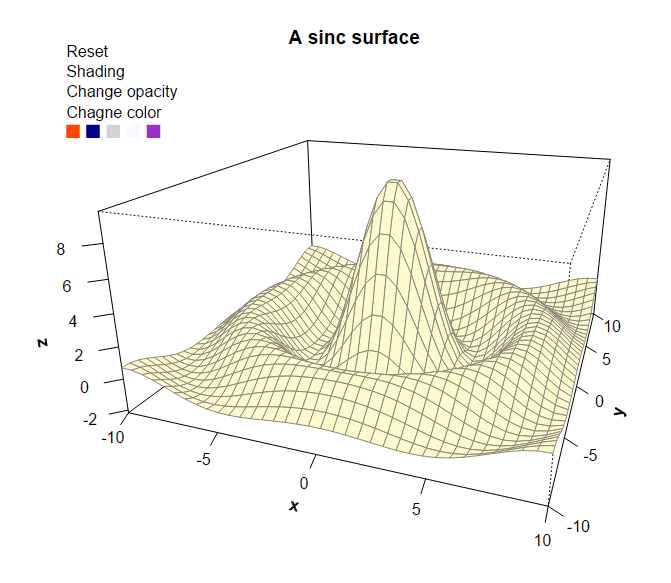
\includegraphics[height = 5cm, width = 5cm]{figure/svg/origin_1.PNG}
		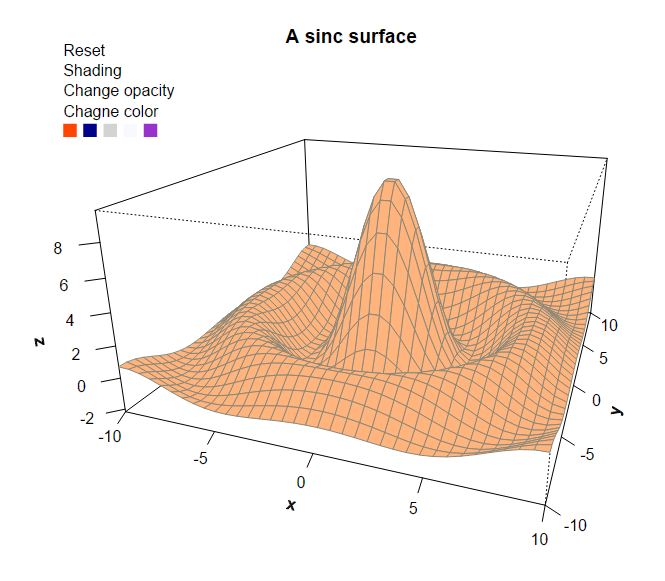
\includegraphics[height = 5cm, width = 5cm]{figure/svg/change_2.PNG}
		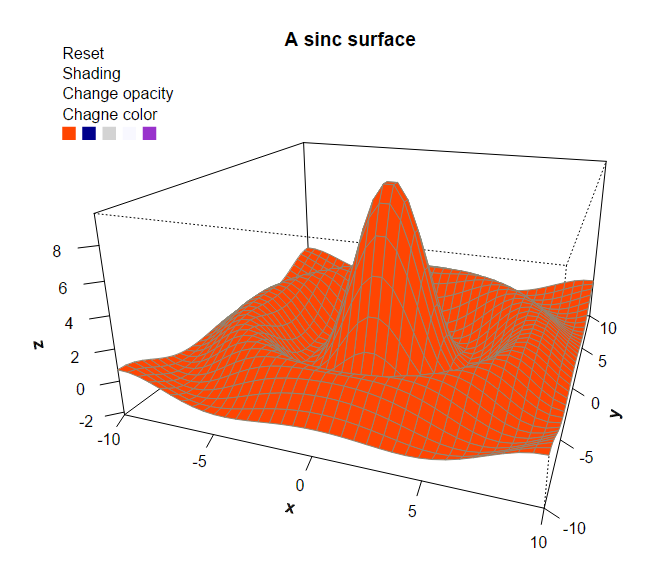
\includegraphics[height = 5cm, width = 5cm]{figure/svg/change_3.PNG}
		\caption{The plot shows the animation that changing the surface color from the left plot to right plot}
		\label{Example_6.3.1}
	\end{center}
\end{figure}

\subsubsection*{Animation of Changing the opacity of the surface}
Similar to the animation of Changing the color of the surface, the opacity attribute of the surface will be change in this example. The animation will be activated when user clicks the "Change opacity" text on the top-left panel of figure \ref{Example_6.3.01}. Once user clicked the text, the \texttt{addAlpha()} will call the \texttt{animate()} which it locates all the polygons and then changes the stroke opacity gradually every 30 milliseconds. (See Figure \ref{Example_6.3.2})
\begin{lstlisting}[language = JavaScript]
animate = function(...){
    setInterval(frame, 30)
    function frame() {
        polygons_odd[i].setAttribute("stroke-opacity", ...);
    }
}

addAlpha = function(){
    animate(action = 'alpha', ...);
}
...
alpha = document.getElementById('alpha.1.1.text');
alpha.onclick = addAlpha; 
\end{lstlisting}

\begin{figure}[h]
	\begin{center}
		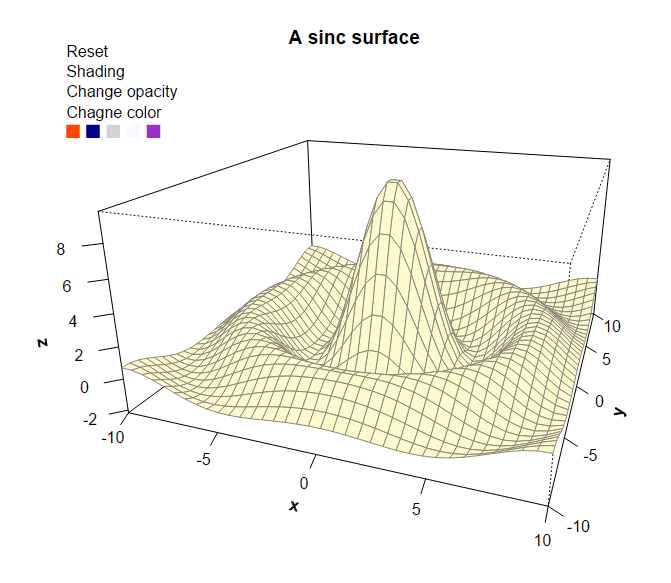
\includegraphics[height = 5cm, width = 5cm]{figure/svg/origin_1.PNG}
		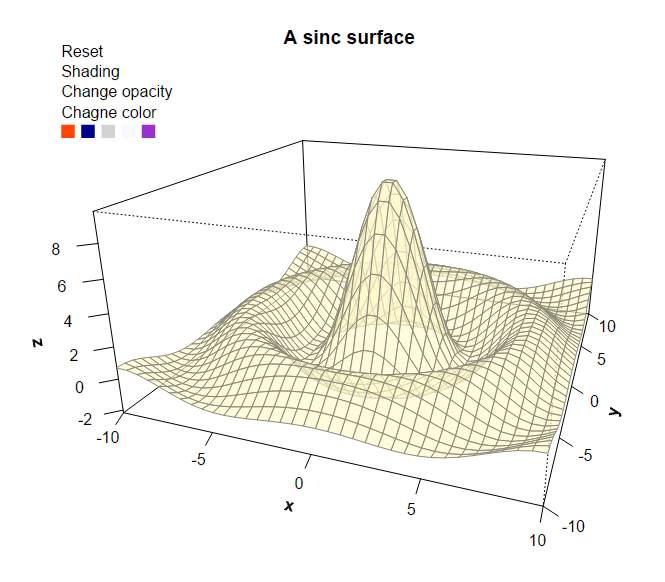
\includegraphics[height = 5cm, width = 5cm]{figure/svg/opacity_2.PNG}
		\includegraphics[height = 5cm, width = 5cm]{figure/svg/opacity_3.PNG}
		\caption{The plot shows the animation that decreasing the opacity of sinc surface from the left plot to right plot}
		\label{Example_6.3.2}
	\end{center}
\end{figure}

\subsubsection*{Animation of shading the surface}
The figure \ref{Example_6.3.3} shows the action of adding shade of the current sinc surface. The middle plot is captured during the duration.
\begin{figure}[h]
	\begin{center}
		\includegraphics[height = 5cm, width = 5cm]{figure/svg/origin_1.PNG}
		\includegraphics[height = 5cm, width = 5cm]{figure/svg/Shade_2.PNG}
		\includegraphics[height = 5cm, width = 5cm]{figure/svg/Shade_3.PNG}
		\caption{The shading animation}
		\label{Example_6.3.3}
	\end{center}
\end{figure}

\subsubsection*{Highlighting the specific fragment of the surface and showing its z-value}
The action of this example will be slightly difference to the previous example. Two actions need to be activated at the same time when user moves the mouse into a specific fragment of the sinc surface. (1) highlighting the fragment. (2) Displaying the its z-value. When the mouse leave the fragment, the color needs to be reset and the z-value needs to be hidden.\\

The trick to perform this action is to display the correct z-value for the specific polygon. The SVG we created is not only a sinc surface and the action text, but also a set of z values, located at the top-right corner of the box. Since their opacity are 0 hence they are invisible at the beginning.\\

First to all, we need to add the \texttt{onmouseover} and the \texttt{onmouseout} events to all fragments. That is, the functions \texttt{polygonon()} and \texttt{polygonout()} are activated when the mouse enter and leave the region of the specific fragments.\\

There are two action will happen when the mouse enters the fragments. One is highlighting the fragment and the other is display its z-value. The highlighting action can be done simply by changing the color of the fragments. The z-value is displayed by matching the correct index. That is, the action function \texttt{polygonon()} will pull out the index of the id attribute from the specific polygon element, and then it will find the label element by matching this index. Finally, the z-value will be displayed by setting the opacity of the label element to be 1. When the mouse leave the fragment, it is necessary to reset the color of this fragment and hide the z-value. These actions will be done by \texttt{polygonout()}.

\begin{lstlisting}[language = JavaScript]
for(i = 1; i <= total; i++){
    obj = document.getElementById('polygon.' + 2 + '.' + i);
    obj.onmouseover = polygonon;
    obj.onmouseout = polygonout;
}
polygonon = function(){
    str = this.id;
    polygon_index = str.replace(/polygon.[0-9]./, '');
    // highlight the polygon
    this.setAttribute('fill', "rgb(255,100,100)");
    // show the 'value'
    label = document.getElementById('labels.' + '1.' + polygon_index + '.text');
    label.setAttribute("fill-opacity",1);
}
polygonout = function(){
    str = this.id;
    polygon_index = str.replace(/polygon.[0-9]./, '');
    // hide the label
    label = document.getElementById('labels.' + '1.' + polygon_index + '.text');
    label.setAttribute("fill-opacity",0);
    opacity = this.getAttribute('fill-opacity');
    // rest the color
    this.setAttribute("fill",window.new_rgb);
}
\end{lstlisting}

\begin{figure}[h]
	\begin{center}
		\includegraphics[height = 7.5cm, width = 7.5cm]{figure/svg/hlight_1.PNG}
		\includegraphics[height = 7.5cm, width = 7.5cm]{figure/svg/hlight_2.PNG}
		\caption{The fragment will be highlight when the mouse move into its area. Also its z-value will be appeared}
		\label{Example_6.3.4}
	\end{center}
\end{figure}

\chapter{Conclusion}

\section{Limitations}
There are couples of things that can be improved: (1). The \textbf{gridGraphics} package cannot fully implement full set of the \textbf{fix up} function. For example, the \texttt{FixupCol()} function which used to fix some unusual colors in some unusual situation, if the some of the colors is missing when shading action happen \texttt{persp()} then those missing colors will be convert to white color ($rgb(1, 1, 1, 1)$). this action will be implement in \texttt{persp()} but the rest fix action may or may not implement by \texttt{persp()}. (2). The \texttt{persp()} is not fully vectorization. The calculation for shading colors is still using loops rather than vectorization. Therefore, it may slow down the software if shading a surface which contains large amounts of polygons. \\


\section{Disscussion}
The \textbf{gridGraphics} is the package to make the connection between \textbf{graphics} and \textbf{grid} package. The \texttt{grid.echo()} function will convert plots drawn by \textbf{graphics} package into \textbf{grid}.\\

There are two kinds of \textbf{graphics} plot that were not supported by previous version: \texttt{persp()} for drawing perspective plot and \texttt{filled.contour()} for drawing level filled contour plot. The surface of perspective plot is formed by finite number of polygons, where polygons have four vertexes. The surface will be drawn by calculating the coordinates of vertices of every polygon. The other features that \texttt{persp()} supported, the lighting, boxes and axis will be emulate by translating \texttt{C} codes to \texttt{R} codes. The surface of filled contour plot will be emulated by translating the \texttt{C} code directly then vectorized so that the function will be more efficient. \\

The core of \textbf{gridGraphics} package provides fully viewport structure to support the filled contour plot. Integrating \texttt{filled.contour()} will be done by navigating to the correct viewport and draw the filled contour plot. However, \textbf{gridGraphics} does not fully provide the viewport structure for \texttt{persp}. The solution to this problem is that: creating a new viewport in the correct location of the viewport tree (created by \textbf{gridGraphics} when \texttt{grid.echo()} been called.). Then we need to consider: (1) The x-scale and y-scale for the viewport. (2) Determined the clipping happens for every component. The x-scale and y-scale will be calculated based on the size of the current graphics device. The solution will be to write a \texttt{R} function that do the extract calculation for the range of x and y (from \textbf{graphics}). The clipping will be solved by observing the difference from the \texttt{persp()} plot that drawn by \textbf{graphics} and \textbf{grid}. That is, the clipping will be turned on when drawing both the axes and box, but it will be turned off when drawing the surface. Finally \texttt{persp()} is integrated into the package by navigating to the viewport with correct scale and correct clipping actions.\\

To ensure the accuracy of identical that a \textbf{graphics} plot redrawn on \textbf{grid}, it is necessary to provide the identical test. The \textbf{ImageMagick} software will be used to test the identical (mathematically and visually) between a \textbf{graphics}-plot and \textbf{grid}-plot. Most kinds of plots are identical mathematically and visually. (See Figure \ref{chapter5.2} and figure \ref{chapter5.3}).

\section*{Availability}
The updated \textbf{gridGraphics} package which supported the conversion of \texttt{persp()} and \texttt{filled.contour()} from \textbf{graphics}-base to \textbf{grid} is now available from CRAN and GitHub. And, the supporting material of this paper, which including the animation of the section 6.3.2 is also available from the following website: \\
\begin{center}
    \herf{https://github.com/yeamin1/MasterProject/tree/master/report/svg} \\
    \herf{https://github.com/yeamin1/gridgraphics} \\
    \herf{https://github.com/pmur002/gridgraphics}\\
\end{center}



\bibliography{reference/reference}
\bibliographystyle{./reference/elsart-harv} 


\chapter{Appendix}
\section{persp.R}
\begin{lstlisting}[language = R]
## initialize and create a viewport prepare for drawing
perInit = function ( plot, newpage = FALSE, dbox = TRUE ) {
    info = plot
    ## [[1]] is the all the grapical information that transfer into grid
    ## [[3]] is the persp call information
    ## [[2]] is the plot details eg: x, y, z, xlim, ylim, zlim, col ...
    ## create a list that store all information from the persp
    ## then pass the information to per for drawing.
    ## x is [[2]]; y is [[3]]; z is [[4]]
    ## xr is [[5]]; yr is [[6]]; zr is [[7]]
    ## col is [[14]]; border is [[15]]; box is [[19]]
    ## axes is [[20]], nTicks is [[21]]
    ## tickType is [[22]]
    ## xlab/ylab/zlab = [[23]]/[[24]]/[[25]]
	## main is in plot[[1]][[4]][[2]][[2]]
    ## shade is 0.8, ltheta/lphi = [[16]]/[[17]]
    ## expand is [[13]], scale is [[12]]
    out = list(x = info[[2]], y = info[[3]], z = info[[4]],
                xr = info[[5]], yr = info[[6]], zr = info[[7]],
                col = info[[14]], border = info[[15]][1] ##only allows one color for border
				, dbox = info[[19]],
                newpage = newpage, 
                phi = info[[9]], theta = info[[8]], r = info[[10]], d = info[[11]],
                axes = info[[20]], nTicks = info[[21]], tickType = info[[22]],
                xlab = info[[23]], ylab = info[[24]], zlab = info[[25]],
				## parameters in 'par' that need added to per
                lwd = info$lwd, lty = info$lty, #col.axis = info$col.axis,
				#col.lab = info$col.lab, 
				cex.lab = info$cex.lab, 
                shade = info[[18]], ltheta = info[[16]], lphi = info[[17]],
                expand = info[[13]], scale = info[[12]]
				#main = plot[[1]][[4]][[2]][[2]]
                )
    
    if(out$newpage == TRUE)
        grid.newpage()
    out
}

## main call 
C_persp = function(plot = NULL, ...)
{
    dev.set(recordDev())
    par = currentPar(NULL)
    dev.set(playDev())
    
    #information extraction
    xc = yc = zc = xs = ys = zs = 0
    plot = perInit(plot, newpage = FALSE)
    xr = plot$xr; yr = plot$yr; zr = plot$zr
    xlab = plot$xlab; ylab = plot$ylab; zlab = plot$zlab
    col.axis = plot$col.axis; col.lab = plot$col.lab; 
    col = plot$col; cex.lab = plot$cex.lab
    nTicks = plot$nTicks; tickType = plot$tickType
    expand = plot$expand ;scale = plot$scale
    ltheta = plot$ltheta; lphi = plot$lphi
    main = plot$main; axes = plot$axes
    dbox = plot$dbox; shade = plot$shade
    r = plot$r; d = plot$d; phi = plot$phi; theta = plot$theta
	
	xs = LimitCheck(xr)[1]
    ys = LimitCheck(yr)[1]
    zs = LimitCheck(zr)[1]
    xc = LimitCheck(xr)[2]
    yc = LimitCheck(yr)[2]
    zc = LimitCheck(zr)[2]
	
	if(scale == FALSE){
		s = xs
		if(s < ys) s = ys
		if (s < zs) s = zs
		xs = s
		ys = s
		zs = s
	}
    
    VT = diag(1, 4)
    VT = VT %*% Translate(-xc, -yc, -zc)
    VT = VT %*% Scale(1/xs, 1/ys, expand/zs)
    VT = VT %*% XRotate(-90.0)
    VT = VT %*% YRotate(-theta)
    VT = VT %*% XRotate(phi)
    VT = VT %*% Translate(0.0, 0.0, -r - d)
    trans = VT %*% Perspective(d)

    border = plot$border[1];
    if(is.null(plot$lwd)) lwd = 1 else lwd = plot$lwd
    if(is.null(plot$lty)) lty = 1 else lty = plot$lty
    if(any(!(is.numeric(xr) & is.numeric(yr) & is.numeric(zr)))) stop("invalid limits")
    if(any(!(is.finite(xr) & is.finite(yr) & is.finite(zr)))) stop("invalid limits")
    
    
    if(!scale) xs = ys = zs = max(xs, ys, zs)
    colCheck = col2rgb(col, alpha = TRUE)[4,1] == 255
    if(is.finite(ltheta) && is.finite(lphi) && is.finite(shade) && colCheck)
    DoLighting = TRUE else DoLighting = FALSE
    ## check the first color act as Fixcols
    
    if (DoLighting) Light = SetUpLight(ltheta, lphi)
    
    # create a viewport inside a 'viewport'
    depth = gotovp(FALSE)
    lim = PerspWindow(xr, yr, zr, trans, 'r')
    #vp = viewport(0.5, 0.5, 1, 1, default.units = 'npc',
    #                xscale = lim[1:2], yscale = lim[3:4])
    upViewport(depth)
    
    incrementWindowAlpha()
    setWindowPlotAlpha(plotAlpha())
    setUpUsr(lim)
    
    if (dbox == TRUE) {
        EdgeDone = rep(0, 12)
        if(axes == TRUE){
            depth = gotovp(TRUE)
            PerspAxes(xr, yr, zr, ##x, y, z
                    xlab, ylab, zlab, ## xlab, xenc, ylab, yenc, zlab, zenc
                    nTicks, tickType, trans, ## nTicks, tickType, VT
                    lwd, lty, col.axis, col.lab, cex.lab) ## lwd, lty, col.axis, col.lab, cex.lab
            upViewport(depth)}
    } else {
        EdgeDone = rep(1, 12)
        xr = yr = zr = c(0,0)
    }
    
    ## draw the behind face first
    ## return the EdgeDone inorder to not drawing the same Edege two times.
    depth = gotovp(TRUE)
    EdgeDone = PerspBox(0, xr, yr, zr, EdgeDone, trans, 1, lwd)
    upViewport(depth)
    
    depth = gotovp(FALSE)
    DrawFacets(plot = plot, z = plot$z, x = plot$x, y = plot$y,     ## basic
                xs = 1/xs, ys = 1/ys, zs = expand/zs,               ## Light
                col = col,                                          ## cols
                ltheta = ltheta, lphi = lphi, Shade = shade, 
                Light = Light, trans = trans, DoLighting = DoLighting)
    upViewport(depth)

    depth = gotovp(TRUE)
    EdgeDone = PerspBox(1, xr, yr, zr, EdgeDone, trans, 'dotted', lwd)
    upViewport(depth)

}

####Shade function
LimitCheck = function ( lim ) {
    ## not finished yet...
    s = 0.5 * abs(lim[2] - lim[1])
    c = 0.5 * (lim[2] + lim[1])
    c(s, c)
}

XRotate = function ( angle ) {
    TT = diag(1, 4)
    rad = angle * pi / 180
    c = cos(rad)
    s = sin(rad)
    TT[2, 2] = c;
    TT[3, 2] = -s;
    TT[3, 3] = c;
    TT[2, 3] = s;
    TT
}

YRotate = function ( angle ) {
    TT = diag(1, 4)
    rad = angle * pi / 180
    c = cos(rad)
    s = sin(rad)
    TT[1, 1] = c;
    TT[3, 1] = s;
    TT[3, 3] = c;
    TT[1, 3] = -s;
    TT
}

ZRotate = function ( angle ) {
    TT = diag(1, 4)
    rad = angle * pi / 180
    c = cos(rad)
    s = sin(rad)
    TT[1, 1] = c;
    TT[2, 1] = -s;
    TT[2, 2] = c;
    TT[1, 2] = s;
    TT
}

Translate = function(x, y, z)
{
    TT = diag(1,4)
    TT[4, 1] = x
    TT[4, 2] = y
    TT[4, 3] = z
    TT

}

Scale = function(x, y, z)
{
    TT = diag(1,4)    
    TT[1, 1] = x
    TT[2, 2] = y
    TT[3, 3] = z
    TT
}

Perspective = function(d)
{
    TT = diag(1,4)
    TT[3, 4] = -1 / d
    TT
}

        
SetUpLight = function ( theta, phi ) {
    u = c(0, -1, 0, 1)
    VT = diag(1, 4)
    VT = VT %*% XRotate(-phi)
    VT = VT %*% ZRotate(theta)
    Light = u %*% VT
}

FacetShade = function( u, v, Shade, Light ) {
    nx = u[2] * v[3] - u[3] * v[2]
    ny = u[3] * v[1] - u[1] * v[3]
    nz = u[1] * v[2] - u[2] * v[1]
    sum = sqrt(nx * nx + ny * ny + nz * nz)
    if (is.finite(sum)){
        if (sum == 0) sum = 1
        }else{Shade = NA}
    
    nx = nx/sum
    ny = ny/sum
    nz = nz/sum
    sum = 0.5 * (nx * Light[1] + ny * Light[2] + nz * Light[3] + 1)
    sum^Shade   
}

shadeCol = function( z, x, y, xs, ys, zs, col, ltheta, lphi, Shade, Light) {
    u = v = 0
    shade = 0
    nx = nrow(z)
    ny = ncol(z)
    nx1 = nx - 1
    ny1 = ny - 1
    cols = 0
    ncol = length(col)
    indx = 0:(length(z))
    Light = SetUpLight(ltheta, lphi)
    for(k in 1:(nx1 * ny1)){
        nv = 0
        i = (indx[k]) %% nx1 
        j = (indx[k]) %/% nx1
        icol = (i + j * nx1) %% ncol + 1

        u[1] = xs * (x[i + 2] - x[i + 1])
	    u[2] = ys * (y[j + 1] - y[j + 2])
	    u[3] = zs * (z[(i + 1)+ j * nx + 1] - z[i + (j + 1) * nx + 1])
	    v[1] = xs * (x[i + 2] - x[i + 1])
	    v[2] = ys * (y[j + 2] - y[j + 1])
	    v[3] = zs * (z[(i + 1) + (j + 1) * nx + 1] - z[i + j * nx + 1])
        icol = (i + j * nx1) %% ncol
	    shade[k] = FacetShade(u, v, Shade = Shade, Light = Light)

        shadedCol = col2rgb(col[icol + 1], alpha = TRUE)
        if(is.finite(shade[k])){
            cols[k] = rgb(shade[k] * shadedCol[1], 
                        shade[k] * shadedCol[2], 
                        shade[k] * shadedCol[3], 
                        maxColorValue = 255)
        }else{
            cols[k] = rgb(1,1,1,0)
                        }
    }
        list(cols = cols, shade = shade)
}

## shade end...
PerspBox = function(front = 1, x, y, z, EdgeDone, VT, lty, lwd = lwd )
{
    u0 = u1 = u2 = u3 = 0
    v0 = v1 = v2 = v3 = 0
    for (f in 1:6) {
        p0 = Face[f, 1]
        p1 = Face[f, 2]
        p2 = Face[f, 3]
        p3 = Face[f, 4]

        u0[1] = x[Vertex[p0, 1]]
        u0[2] = y[Vertex[p0, 2]]
        u0[3] = z[Vertex[p0, 3]]
        u0[4] = 1
        u1[1] = x[Vertex[p1, 1]]
        u1[2] = y[Vertex[p1, 2]]
        u1[3] = z[Vertex[p1, 3]]
        u1[4] = 1
        u2[1] = x[Vertex[p2, 1]]
        u2[2] = y[Vertex[p2, 2]]
        u2[3] = z[Vertex[p2, 3]]
        u2[4] = 1
        u3[1] = x[Vertex[p3, 1]]
        u3[2] = y[Vertex[p3, 2]]
        u3[3] = z[Vertex[p3, 3]]
        u3[4] = 1

        v0 = TransVector(u0, VT)
        v1 = TransVector(u1, VT)
        v2 = TransVector(u2, VT)
        v3 = TransVector(u3, VT)
        
        v0 = v0/v0[4]
        v1 = v1/v1[4]
        v2 = v2/v2[4]
        v3 = v3/v3[4]
        
        d = v1 - v0
        e = v2 - v1
        
        nearby = (d[1]*e[2] - d[2]*e[1]) < 0
        
        ## draw the face line by line rather than polygon
        if ((front && nearby) || (!front && !nearby)) {
            if (!EdgeDone[Edge[f, 1]]){
                grid.lines(c(v0[1], v1[1]), c(v0[2], v1[2]), default.units = 'native',
                    gp = gpar(lty = lty, lwd = lwd) 
                    )
                EdgeDone[Edge[f, 1]] = EdgeDone[Edge[f, 1]] + 1
                }
            if (!EdgeDone[Edge[f, 2]]){
                grid.lines(c(v1[1], v2[1]), c(v1[2], v2[2]), default.units = 'native',
                    gp = gpar(lty = lty, lwd = lwd) 
                    )
                EdgeDone[Edge[f, 2]] = EdgeDone[Edge[f, 2]] + 1
                }
            if (!EdgeDone[Edge[f, 3]]){
                grid.lines(c(v2[1], v3[1]), c(v2[2], v3[2]), default.units = 'native',
                    gp = gpar(lty = lty, lwd = lwd) 
                    )
                EdgeDone[Edge[f, 3]] = EdgeDone[Edge[f, 3]] + 1
                }
            if (!EdgeDone[Edge[f, 4]]){
                grid.lines(c(v3[1], v0[1]), c(v3[2], v0[2]), default.units = 'native',
                    gp = gpar(lty = lty, lwd = lwd)
                    )
                EdgeDone[Edge[f, 4]] = EdgeDone[Edge[f, 4]] + 1
                }
        }
    }
    EdgeDone
}

dPolygon = function(x, y, z, col, trans){

    ## the total number of polygon that we need to draw	
	nx = length(x)
	ny = length(y)
    total = nx * ny
	stops = (nx - 1) * (ny - 1)

    ## set the temp value for x,y,z prepare for subsetting
    xTmp = rep(x, length(y))
    yTmp = rep(y,each = nx)
    zTmp = as.numeric(z)
    
    ## the drawing order is along x-axis, and then along y-axis
    ## then create a vector like a 4Xn matrix, 
    ## i.e the first column contain all the first points for every polygons
    ## the second column contain all the second points for every polygons and so on 
    pBreak = c(1:total, 1 + 1:total, 1 + nx + 1:total, nx + 1:total)
    xBreak = xTmp[pBreak]
    yBreak = yTmp[pBreak]
    zBreak = zTmp[pBreak]
    
    ## draw the box if required
    ## the vectors now has four paths, every paths contain the information of every points of every polygon
    ## now we need to change the order of this vector, so that the first four index should be the order for drawing 
    ## the first points, not the first four points for the first four polygon
    ## points subsetting 
    plot.index = rep(
        c(1, 1 + total, 
        1 + 2 * total, 
        1 + 3 * total ),
        total) + rep(0:(total - 1), each = 4)

    ## sequence for 'problem's polygons index, e.g
    ## along x-axis, there are n-1 polygons, n is the number of points in x direction
    ## we don't want to draw the nth polygon, hence we deleted those polygon
    dp = rep((4 * seq(nx,total,nx)), each = 4) - (3:0)

    ## final subsetting
    xCoor = xBreak[plot.index][-dp][1 : (4 * stops)]
    yCoor = yBreak[plot.index][-dp][1 : (4 * stops)]
    zCoor = zBreak[plot.index][-dp][1 : (4 * stops)]
    
    ## vectorize the cols
    colRep = rep_len(col, length(xCoor))
    
    ## use the first corner of every polygon to determind the order for drawing
    corn.id = 4* 1:(length(xCoor)/4)
    xc = xCoor[corn.id]
    yc = yCoor[corn.id]
    
    ## method for using the zdepth for changing the drawing order for every polygon
    orderTemp = cbind(xc, yc, 0, 1) %*% trans 
    zdepth = orderTemp[, 4]

    ## the zdepth of a set of 4 points of each polygon
    a = order(zdepth, decreasing = TRUE)
    oo = rep(1:4, length(a)) + rep(a - 1, each = 4) * 4

    xyCoor = trans3d(xCoor[oo],
                    yCoor[oo],
                    zCoor[oo], trans)
                    
    colRep = colRep[a]
    
    ## record the total number of polygon
    pMax = length(xyCoor$x) / 4
    pout = list(xyCoor = xyCoor, pMax = pMax, 
                colRep = colRep, polygonOrder = a)
    pout
}

DrawFacets = function(plot, z, x, y, xs, ys, zs, 
                        col, ltheta, lphi, Shade,
                        Light, trans, DoLighting)
{
    pout = dPolygon(x, y, z, col, trans)
    xyCoor = pout$xyCoor
    pMax = pout$pMax; colRep = pout$colRep
    polygonOrder = pout$polygonOrder
    polygons = cbind(xyCoor$x, xyCoor$y)
    polygon.id = rep(1:pMax, each = 4)
    col = plot$col
    
    if (DoLighting == TRUE) {
        col[is.na(col)] = rgb(1, 1, 1)
        if(is.finite(Shade) && Shade <= 0 ) Shade = 1
        shadding = shadeCol(z, x, y,                       ## x, y, z
                xs, ys, zs,                                 ## xs, ys, zs 
                col,                           ## col, ncol
                ltheta, lphi, Shade, Light = Light)         ## ltheta, lphi, Shade(not shade)
        shadedCol = shadding[[1]]
        
        ## clean if any NA's Z-value
        shade = shadding[[2]][polygonOrder]
        misshade = !is.finite(shade)
        misindex = rep(misshade, each = 4)
        polygonOrder = polygonOrder[!misshade]
        polygons = polygons[!misindex,]
        polygon.id = polygon.id[!misindex]
        
        cols = shadedCol[polygonOrder]        
    } else {
        cols = rep_len(col, length(polygons[,1]))[polygonOrder]
    }
    
    xrange = range(polygons[,1], na.rm = TRUE)
    yrange = range(polygons[,2], na.rm = TRUE)

    grid.polygon(polygons[,1], polygons[,2], id = polygon.id,
                    default.units = 'native', 
                    gp = gpar(col = plot$border, fill = cols, 
                                lty = plot$lty, lwd = plot$lwd)
                    )
	
}


TransVector = function(u, T) {
    u %*% T
}

lowest = function (y1, y2, y3, y4) {
    (y1 <= y2) && (y1 <= y3) && (y1 <= y4)		
}

labelAngle = function(x1, y1, x2, y2){  

    dx = abs(x2 - x1)
    if ( x2 > x1 ) {
        dy = y2 - y1
    } else {
        dy = y1 - y2
    }
    
    if (dx == 0) {
        if( dy > 0 ) {
            angle = 90
        } else {
            angle = 270
        }
    } else {
        angle = 180/pi * atan2(dy, dx)
    }
    angle
}	

PerspAxis = function(x, y, z, axis, axisType, 
                    nTicks, tickType, label, 
                    VT, lwd = 1, lty, col.axis = 1,
                    col.lab = 1, cex.lab = 1){

    ## don't know how to use numeric on the switch...
    axisType = as.character(axisType)
    tickType = as.character(tickType)
    u1 = u2 = u3 = c(0.,0.,0.,0.)
    tickLength = .03
    
    switch(axisType,
           '1' = {min = x[1]; max = x[2]; range = x},
           '2' = {min = y[1]; max = y[2]; range = y},
           '3' = {min = z[1]; max = z[2]; range = z}
            )
            
    d_frac = 0.1 * (max - min)
    nint = nTicks - 1
    
    if(!nint)nint = nint + 1
    i = nint

    ticks = axisTicks(c(min, max), FALSE, nint = nint)
    min = ticks[1]
    max = ticks[length(ticks)]
    nint = length(ticks) - 1
            
    ## but maybe not this one... haven't test yet...
    while((min < range[1] - d_frac || range[2] + d_frac < max) && i < 20) {
        nint = i + 1
        ticks = axisTicks(c(min, max), FALSE)
        range = range(ticks)
        nint = length(ticks) - 1
    }
    
    ## axp seems working...
    axp = 0
    axp[1] = min
    axp[2] = max
    axp[3] = nint
    
    # Do the following calculations for both ticktypes
    # Vertex is a 8*3 matrix; i.e. the vertex of a box
    # AxisStart is a vector of length 8
    # axis is a output 
    # u1, u2 are the vectors in 3-d 
    # the range of x,y,z
    switch (axisType,
        '1' = {
          u1[1] = min
          u1[2] = y[Vertex[AxisStart[axis], 2]]
          u1[3] = z[Vertex[AxisStart[axis], 3]]
        },
        '2' = {
          u1[1] = x[Vertex[AxisStart[axis], 1]]
          u1[2] = min
          u1[3] = z[Vertex[AxisStart[axis], 3]]
        },
        '3' = {
          u1[1] = x[Vertex[AxisStart[axis], 1]]
          u1[2] = y[Vertex[AxisStart[axis], 2]]
          u1[3] = min
        }
    )
    u1[1] = u1[1] + tickLength*(x[2]-x[1])*TickVector[axis, 1]
    u1[2] = u1[2] + tickLength*(y[2]-y[1])*TickVector[axis, 2]
    u1[3] = u1[3] + tickLength*(z[2]-z[1])*TickVector[axis, 3]
    u1[4] = 1

    ##axisType, 1 = 'draw x-axis'
    ##          2 = 'draw y-axis'
    ##          3 = 'draw z-axis'
    switch (axisType,
        '1' = {
        u2[1] = max
        u2[2] = u1[2]
        u2[3] = u1[3]
        },
        '2' = {
        u2[1] = u1[1]
        u2[2] = max
        u2[3] = u1[3]
        },
        '3' = {
        u2[1] = u1[1]
        u2[2] = u1[2]
        u2[3] = max
        }
    )
    u2[4] = 1

    switch(tickType,
        '1' = { 
        u3[1] = u1[1] + tickLength*(x[2]-x[1])*TickVector[axis, 1]
        u3[2] = u1[2] + tickLength*(y[2]-y[1])*TickVector[axis, 2]
        u3[3] = u1[3] + tickLength*(z[2]-z[1])*TickVector[axis, 3]
        },
        '2' = {
        u3[1] = u1[1] + 2.5*tickLength*(x[2]-x[1])*TickVector[axis, 1]
        u3[2] = u1[2] + 2.5*tickLength*(y[2]-y[1])*TickVector[axis, 2]
        u3[3] = u1[3] + 2.5*tickLength*(z[2]-z[1])*TickVector[axis, 3]
        }
    )

    ## u3 is the the labels at the center of each axes
    switch(axisType,
        '1' = {
        u3[1] = (min + max)/2
        },
        '2' = {
        u3[2] = (min + max)/2
        },
        '3' = {
        u3[3] = (min + max)/2
        }
    )
    u3[4] = 1

    ## transform the 3-d into 2-d
    v1 = TransVector(u1, VT)
    v2 = TransVector(u2, VT)
    v3 = TransVector(u3, VT)

    v1 = v1/v1[4]
    v2 = v2/v2[4]
    v3 = v3/v3[4]
      
    ## label at center of each axes
    srt = labelAngle(v1[1], v1[2], v2[1], v2[2])
    #text(v3[1], v3[2], label, 0.5, srt = srt)
    grid.text(label = label, x = v3[1], y = v3[2],
          just = "centre", rot = srt,
          default.units = "native", #vp = 'clipoff',
          gp = gpar(col = col.lab, lwd = lwd, cex = cex.lab)
          )
    
    ## tickType is not working.. when = '2'
    switch(tickType,
    '1' = {
    arrow = arrow(angle = 10, length = unit(0.1, "in"),
                    ends = "last", type = "open")  
	## drawing the tick..
    
    grid.lines(x = c(v1[1], v2[1]), y = c(v1[2], v2[2]),
          default.units = "native", arrow = arrow, #vp = 'clipoff',
          gp = gpar(col = 1, lwd = lwd , lty = lty )
          )
       },
    ## '2' seems working
    '2' = {
        at = axisTicks(range, FALSE, axp, nint = nint)
        lab = format(at, trim = TRUE)
        for(i in 1:length(at)){
            switch(axisType, 
                '1' = {
                u1[1] = at[i]
                u1[2] = y[Vertex[AxisStart[axis], 2]]
                u1[3] = z[Vertex[AxisStart[axis], 3]]
                },
                '2' = {
                u1[1] = x[Vertex[AxisStart[axis], 1]]
                u1[2] = at[i]
                u1[3] = z[Vertex[AxisStart[axis], 3]]
                },
                '3' = {
                u1[1] = x[Vertex[AxisStart[axis], 1]]
                u1[2] = y[Vertex[AxisStart[axis], 2]]
                u1[3] = at[i]
                }
            )
            
            tickLength = 0.03
            
            u1[4] = 1
            u2[1] = u1[1] + tickLength*(x[2]-x[1])*TickVector[axis, 1]
            u2[2] = u1[2] + tickLength*(y[2]-y[1])*TickVector[axis, 2]
            u2[3] = u1[3] + tickLength*(z[2]-z[1])*TickVector[axis, 3]
            u2[4] = 1
            u3[1] = u2[1] + tickLength*(x[2]-x[1])*TickVector[axis, 1]
            u3[2] = u2[2] + tickLength*(y[2]-y[1])*TickVector[axis, 2]
            u3[3] = u2[3] + tickLength*(z[2]-z[1])*TickVector[axis, 3]
            u3[4] = 1
            v1 = TransVector(u1, VT)
            v2 = TransVector(u2, VT)
            v3 = TransVector(u3, VT)
                        
            v1 = v1/v1[4]
            v2 = v2/v2[4]
            v3 = v3/v3[4]
            
            ## Draw tick line
            grid.lines(x = c(v1[1], v2[1]), y = c(v1[2], v2[2]),
                default.units = "native", ##vp = 'clipoff',
                gp = gpar(col = col.axis, lwd = lwd, lty = lty)
                )

            ## Draw tick label
            grid.text(label = lab[i], x = v3[1], y = v3[2],
                just = "centre",
                default.units = "native", #vp = 'clipoff',
                gp = gpar(col = col.axis, adj = 1, pos = 0.5, cex = 1)
                )
            }
        }
    )
}


PerspAxes = function(x, y, z, 
                    xlab, 
                    ylab, 
                    zlab, 
                    nTicks, tickType, VT, 
					## parameters in par
                    lwd = 1, lty = 1, col.axis = 1, col.lab = 1, cex.lab = 1)
{
    xAxis = yAxis = zAxis = 0 ## -Wall 
    u0 = u1 = u2 = u3 = 0

    u0[1] = x[1]; u0[2] = y[1]; u0[3] = z[1]; u0[4] = 1
    u1[1] = x[2]; u1[2] = y[1]; u1[3] = z[1]; u1[4] = 1
    u2[1] = x[1]; u2[2] = y[2]; u2[3] = z[1]; u2[4] = 1
    u3[1] = x[2]; u3[2] = y[2]; u3[3] = z[1]; u3[4] = 1

    v0 = TransVector(u0, VT)
    v1 = TransVector(u1, VT)
    v2 = TransVector(u2, VT)
    v3 = TransVector(u3, VT)

    v0 = v0/v0[4]
    v1 = v1/v1[4]
    v2 = v2/v2[4]
    v3 = v3/v3[4]

    if (lowest(v0[2], v1[2], v2[2], v3[2])) {
        xAxis = 1
        yAxis = 2
    } else if (lowest(v1[2], v0[2], v2[2], v3[2])) {
        xAxis = 1
        yAxis = 4
    } else if (lowest(v2[2], v1[2], v0[2], v3[2])) {
        xAxis = 3
        yAxis = 2
    } else if (lowest(v3[2], v1[2], v2[2], v0[2])) {
        xAxis = 3
        yAxis = 4
    } else
        warning("Axis orientation not calculated")
    ## drawing x and y axes
    PerspAxis(x, y, z, xAxis, '1', nTicks, tickType, xlab, VT, 
                lwd = lwd, lty = lty, col.axis = col.axis, 
                col.lab = col.lab, cex.lab = cex.lab)
                
    PerspAxis(x, y, z, yAxis, '2', nTicks, tickType, ylab, VT, 
                lwd = lwd, lty = lty, col.axis = col.axis, 
                col.lab = col.lab, cex.lab = cex.lab)

    ## Figure out which Z axis to draw
    if (lowest(v0[1], v1[1], v2[1], v3[1])) {
            zAxis = 5
        }else if (lowest(v1[1], v0[1], v2[1], v3[1])) {
            zAxis = 6
        }else if (lowest(v2[1], v1[1], v0[1], v3[1])) {
            zAxis = 7
        }else if (lowest(v3[1], v1[1], v2[1], v0[1])) {
            zAxis = 8
        }else
    warning("Axis orientation not calculated")

    ## drawing the z-axis
    PerspAxis(x, y, z, zAxis, '3', nTicks, tickType, zlab, VT, 
                lwd = lwd, lty = lty, col.axis = col.axis, 
                col.lab = col.lab, cex.lab = cex.lab)
}


PerspWindow = function(xlim, ylim, zlim, VT, style)
{
    xmax = xmin = ymax = ymin = u = 0
    u[4] = 1
    for (i in 1:2) {
        u[1] = xlim[i]
        for (j in 1:2) {
            u[2] = ylim[j]
            for (k in 1:2) {
                u[3] = zlim[k]
                v = TransVector(u, VT)
                xx = v[1] / v[4]
                yy = v[2] / v[4]
                if (xx > xmax) xmax = xx
                if (xx < xmin) xmin = xx
                if (yy > ymax) ymax = yy
                if (yy < ymin) ymin = yy
          }
        }
    }
    pin1 = convertX(unit(1.0, 'npc'), 'inches', valueOnly = TRUE)
    pin2 = convertY(unit(1.0, 'npc'), 'inches', valueOnly = TRUE)
    xdelta = abs(xmax - xmin)
    ydelta = abs(ymax - ymin)
    xscale = pin1 / xdelta
    yscale = pin2 / ydelta
    scale = if(xscale < yscale) xscale else yscale
    xadd = .5 * (pin1 / scale - xdelta);
    yadd = .5 * (pin2 / scale - ydelta);
    ## GScale in C
    xrange = GScale(xmin - xadd, xmax + xadd, style)
    yrange = GScale(ymin - yadd, ymax + yadd, style)
    c(xrange, yrange)
  
}

GScale = function(min, max, style)
{
  switch(style, 
         'r' = {temp = 0.04 * (max - min)
         min = min - temp
         max = max + temp
         },
         'i' = {}
  )
  c(min, max)
}


## global variables.
TickVector = matrix(ncol = 3, byrow = TRUE, data = c(
    0, -1, -1,
    -1, 0, -1,
    0, 1, -1,
    1, 0, -1,
    -1, -1, 0,
    1, -1, 0,
    -1, 1, 0,
    1, 1, 0 ))

Vertex = matrix(ncol = 3, byrow = TRUE, data = c(
	1, 1, 1,  #xlim[1], ylim[1], zlim[1]
	1, 1, 2,  #xlim[1], ylim[1], zlim[2]
	1, 2, 1,
	1, 2, 2,
	2, 1, 1,
	2, 1, 2,
	2, 2, 1,
	2, 2, 2 ))

Face  = matrix (ncol = 4, byrow = TRUE, data = c(
    1, 2, 6, 5,
    3, 7, 8, 4,
    1, 3, 4, 2,
    5, 6, 8, 7,
    1, 5, 7, 3,
    2, 4, 8, 6 ))

Edge  = matrix (ncol = 4, byrow = TRUE, data = c(
    0, 1, 2, 3,
    4, 5, 6, 7,
    8, 7, 9, 0,
    2,10, 5,11,
    3,11, 4, 8,
    9, 6,10, 1)) + 1
    
AxisStart = c(1, 1, 3, 5, 1, 5, 3, 7)
\end{lstlisting}
\newpage
\section{filled.contour.R}
\begin{lstlisting}[language = R]
## vectorization version  (main in used)
FindPolygonVertices = function(low,  high,
		     x1,  x2,  y1,  y2,
		     z11,  z21,  z12,  z22,
             colrep){

    v1 = FindCutPoints(low, high, x1, y1, x2, y1, z11, z21)
    v2 = FindCutPoints(low, high, y1, x2, y2, x2, z21, z22)
    v3 = FindCutPoints(low, high, x2, y2, x1, y2, z22, z12)
    v4 = FindCutPoints(low, high, y2, x1, y1, x1, z12, z11)

    vx = cbind(v1[[1]], v2[[2]], v3[[1]], v4[[2]])
    vy = cbind(v1[[2]], v2[[1]], v3[[2]], v4[[1]])
    
    ##  track the coordinate for x and y( if non-NA's)
    index = rowSums(!is.na(vx) )
    ## keep if non-NAs row >= 2 (npt >= 2)
    vx = t(vx)
    vy = t(vy)
    xcoor.na = as.vector(vx[, index > 2])
    ycoor.na = as.vector(vy[, index > 2])
    ## delete all NA's,
    xcoor = xcoor.na[!is.na(xcoor.na)]
    ycoor = ycoor.na[!is.na(ycoor.na)]

    id.length = index[index > 2]
    cols = colrep[index > 2]
    
    out = list(x = xcoor, y = ycoor, id.length = id.length, cols = cols)
    outs = out
    out
}

FindCutPoints = function(low, high, x1, y1, x2, y2, z1, z2)
{
## inner condiction begin
    ## first ocndiction
    c = (z1 - high) / (z1 - z2)
    cond1 = z1 < high
    cond2 = z1 == Inf
    cond3 = z2 > high | z1 < low
    
    x.1 = ifelse(cond1, x1, 
              ifelse(cond2, x2, x1 + c * (x2 - x1)))
    x.1 = ifelse(cond3, NA, x.1)
                
    y.1 = ifelse(cond1, y1, 
               ifelse(cond2, y1, y1))
    y.1 = ifelse(cond3, NA, y.1)
    
    cond4 = z2 == -Inf
    cond5 = z2 <= low
    cond6 = z2 > high | z1 < low

    c = (z2 -low) / (z2 - z1)
    x.2 = ifelse(cond4, x1,
             ifelse(cond5, x2 - c * (x2 - x1), NA))
    x.2 = ifelse(cond6, NA, x.2)
             
    y.2 = ifelse(cond4, y1,
              ifelse(cond5, y1, NA))
    y.2 = ifelse(cond6, NA, y.2)

    ## second condiction
    cond7 = z1 > low
    cond8 = z1 == -Inf
    cond9 = z2 < low | z1 > high
    
    c = (z1 - low) / (z1 - z2)
    x_1 = ifelse(cond7, x1, 
                ifelse(cond8, x2, x1 + c * (x2 - x1)))
    x_1 = ifelse(cond9, NA, x_1)
                
    y_1 = ifelse(cond7, y1, 
                ifelse(cond8, y1, y1))
    y_1 = ifelse(cond9, NA, y_1)
    
    cond10 = z2 < high
    cond11 = z2 == Inf
    cond12 = z2 < low | z1 > high
                
    c = (z2 - high) / (z2 - z1)
    x_2 = ifelse(cond10, NA, 
                ifelse(cond11, x1, x2 - c * (x2 - x1)))
    x_2 = ifelse(cond12, NA, x_2)
                
    y_2 = ifelse(cond10, NA, 
                ifelse(cond11, y1, y1))
    y_2 = ifelse(cond12, NA, y_2)
                
    ## third condiction
    cond13 = low <= z1 & z1 <= high
    x..1 = ifelse(cond13, x1, NA)
    y..1 = ifelse(cond13, y1, NA)
## inner condiction end
    
## outer condiction 
    cond14 = z1 > z2
    cond15 = z1 < z2

    xout.1 = ifelse(cond14, x.1,
                ifelse(cond15, x_1,
                        x..1))
    xout.2 = ifelse(cond14, x.2,
                ifelse(cond15, x_2,
                        NA))						

    yout.1 = ifelse(cond14, y.1,
                ifelse(cond15, y_1,
                        y..1))
    yout.2 = ifelse(cond14, y.2,
                ifelse(cond15, y_2,
                        NA))			
## outer condiction end

    ## return x1, x2, y1, y2
    xout = cbind(xout.1, xout.2)
    yout = cbind(yout.1, yout.2)
    list(xout, yout)
}

C_filledcontour = function(plot)
{
    dev.set(recordDev())
    par = currentPar(NULL)
    dev.set(playDev())

    x = plot[[2]]
    y = plot[[3]]
    z = plot[[4]]
    s = plot[[5]]
    cols = plot[[6]]
    
    ns = length(s)
    nx = length(x)
    ny = length(y)

    x1 = rep(x[-nx], each = ny - 1)
    x2 = rep(x[-1], each = ny - 1)
    y1 = rep(y[-ny], nx - 1)
    y2 = rep(y[-1], nx - 1)

    z11 = as.numeric(t(z[-nx, -ny]))
    z21 = as.numeric(t(z[-1, -ny ]))
    z12 = as.numeric(t(z[-nx, -1]))
    z22 = as.numeric(t(z[-1, -1]))
    
    x1 = rep(x1, each = ns - 1)
    x2 = rep(x2, each = ns - 1)
    y1 = rep(y1, each = ns - 1)
    y2 = rep(y2, each = ns - 1)
    z11 = rep(z11, each = ns - 1)
    z12 = rep(z12, each = ns - 1)
    z21 = rep(z21, each = ns - 1)
    z22 = rep(z22, each = ns - 1)
    low = rep(s[-ns], (nx - 1) * (ny - 1))
    high = rep(s[-1], (nx - 1) * (ny - 1))
    
    ## rep color until the same length of x, then subsetting 
    if(length(cols) > ns){
        cols = cols[1:(ns - 1)]
    }else
    {
        cols = rep_len(cols, ns - 1)
    }
    colrep = rep(cols[1:(ns - 1)], nx * ny)
    ## feed color as well as subseeting as x and y
    out = FindPolygonVertices(
                low = low, high = high,
                x1 = x1, x2 = x2, 
                y1 = y1, y2 = y2,
                z11 = z11, z21 = z21, 
                z12 = z12, z22 = z22, colrep = colrep)
    ## actual drawing
    depth = gotovp(TRUE)
    grid.polygon(out$x, out$y, default.units = 'native', id.lengths = out$id.length,
             gp = gpar(fill = out$cols, col = NA))
    upViewport(depth)
}


## for loop version
## identical to C_filledcontour in plot3d.c but very slow
lFindPolygonVertices = function(low,  high,
		     x1,  x2,  y1,  y2,
		     z11,  z21,  z12,  z22,
		     x,  y,  z, npt)
{
    out = list()
    npt = 0
    out1 = lFindCutPoints(low, high, x1,  y1,  z11, x2,  y1,  z21, x, y, z, npt)
    x = out1$x; y = out1$y; z = out1$z; npt = out1$npt

    out2 = lFindCutPoints(low, high, y1,  x2,  z21, y2,  x2,  z22, y, x, z, npt)
    x = out2$x; y = out2$y; z = out2$z; npt = out2$npt

    out3 = lFindCutPoints(low, high, x2,  y2,  z22, x1,  y2,  z12, x, y, z, npt)
    x = out3$x; y = out3$y; z = out3$z; npt = out3$npt
            
    out4 = lFindCutPoints(low, high, y2,  x1,  z12, y1,  x1,  z11, y, x, z, npt)

    out$x = out1$x + out2$y + out3$x + out4$y
    out$y = out1$y + out2$x + out3$y + out4$x
    out$npt = out4$npt
    out
}

lC_filledcontour = function(plot)
{
    dev.set(recordDev())
    par = currentPar(NULL)
    dev.set(playDev())

    x  =  plot[[2]]
    y = plot[[3]]
    z = plot[[4]]
    sc = plot[[5]]
    px = py = pz = numeric(8)
    scol = plot[[6]]

    nx = length(x)
    ny = length(y)
    if (nx < 2 || ny < 2) stop("insufficient 'x' or 'y' values")

    ## do it this way as coerceVector can lose dims, e.g. for a list matrix
    if (nrow(z) != nx || ncol(z) != ny) stop("dimension mismatch")

    nc = length(sc)
    if (nc < 1) warning("no contour values")

    ncol = length(scol)
    
    depth = gotovp(TRUE)
    for(i in 1:(nx - 1)){
    for(j in 1:(ny - 1)){
        for(k in 1:(nc - 1)){
            npt = 0
            out = lFindPolygonVertices(sc[k], sc[k + 1],
                    x[i], x[i + 1],
                    y[j], y[j + 1],
                    z[i, j],
                    z[i + 1, j],
                    z[i, j + 1],
                    z[i + 1, j + 1],
                    px, py, pz, npt)
            
            npt = out$npt
            
            if(npt > 2)
            { 
                grid.polygon(out$x[1:npt], out$y[1:npt], default.units = 'native',
                    gp = gpar(fill = scol[(k - 1) %% ncol + 1], col = NA), name = 'filled.contour')
            }
        }
    }
    }
    upViewport(depth)
   
}

lFindCutPoints = function( low,  high,
	       x1,  y1,  z1,
	       x2,  y2,  z2,
	       x,  y,  z,
	       npt)
{
    x = y = z = numeric(8)
    if (z1 > z2 ) {
        if (z2 > high || z1 < low){
            return(out = list(x = x, y = y, z = z, npt = npt))
        }

        if (z1 < high) {
            x[npt + 1] = x1
            y[npt + 1] = y1
            z[npt + 1] = z1
            npt = npt + 1
        } else if (z1 == Inf) {
            x[npt + 1] = x2
            y[npt + 1] = y1
            z[npt + 1] = z2
            npt = npt + 1
        } else {
            c = (z1 - high) / (z1 - z2)
            x[npt + 1] = x1 + c * (x2 - x1)
            y[npt + 1] = y1
            z[npt + 1] = z1 + c * (z2 - z1)
            npt = npt + 1
        }
        
        if (z2 == -Inf) {
            x[npt + 1] = x1
            y[npt + 1] = y1
            z[npt + 1] = z1
            npt = npt + 1
        } else if (z2 <= low) {
            c = (z2 -low) / (z2 - z1)
            x[npt + 1] = x2 - c * (x2 - x1)
            y[npt + 1] = y1
            z[npt + 1] = z2 - c * (z2 - z1)
            npt = npt + 1
        }
        
    } else if (z1 < z2) {
        if (z2 < low || z1 > high) {
                return(out = list(x = x, y = y, z = z, npt = npt))
        }
        
        if (z1 > low) {
            x[npt + 1] = x1
            y[npt + 1] = y1
            z[npt + 1] = z1
            npt = npt + 1
        } else if (z1 == -Inf) {
            x[npt + 1] = x2
            y[npt + 1] = y1
            z[npt + 1] = z2
            npt = npt + 1
        } else { 
            c = (z1 - low) / (z1 - z2)
            x[npt + 1] = x1 + c * (x2 - x1)
            y[npt + 1] = y1
                z[npt + 1] = z1 + c * (z2 - z1)
            npt = npt + 1
        }
        
        if (z2 < high) {
        } else if (z2 == Inf) {
            x[npt + 1] = x1
            y[npt + 1] = y1
            z[npt + 1] = z1
            npt = npt + 1
        } else {
            c = (z2 - high) / (z2 - z1)
            x[npt + 1] = x2 - c * (x2 - x1)
            y[npt + 1] = y1
            z[npt + 1] = z2 - c * (z2 - z1)
            npt = npt + 1
        }
    } else {
        if(low <= z1 && z1 <= high) {
            x[npt + 1] = x1
            y[npt + 1] = y1
            z[npt + 1] = z1
            npt = npt + 1
        }
    }
    out = list(x = x, y = y, z = z, npt = npt)
    out
}
\end{lstlisting}
\end{document}
